%%%%%%%%%%%%%%%%%%%%%%%%%%%%%%%%%%%%%%%%%
% Masters/Doctoral Thesis 
% LaTeX Template
% Version 2.2 (21/11/15)
%
% This template has been downloaded from:
% http://www.LaTeXTemplates.com
%
% Version 2.x major modifications by:
% Vel (vel@latextemplates.com)
%
% This template is based on a template by:
% Steve Gunn (http://users.ecs.soton.ac.uk/srg/softwaretools/document/templates/)
% Sunil Patel (http://www.sunilpatel.co.uk/thesis-template/)
%
% Template license:
% CC BY-NC-SA 3.0 (http://creativecommons.org/licenses/by-nc-sa/3.0/)
%
%%%%%%%%%%%%%%%%%%%%%%%%%%%%%%%%%%%%%%%%%

%----------------------------------------------------------------------------------------
%	PACKAGES AND OTHER DOCUMENT CONFIGURATIONS
%----------------------------------------------------------------------------------------

\documentclass[
10pt, % The default document font size, options: 10pt, 11pt, 12pt
oneside, % Two side (alternating margins) for binding by default, uncomment to switch to one side
english, % ngerman for German
doublespacing, % Single line spacing, alternatives: onehalfspacing or doublespacing
%draft, % Uncomment to enable draft mode (no pictures, no links, overfull hboxes indicated)
%nolistspacing, % If the document is onehalfspacing or doublespacing, uncomment this to set spacing in lists to single
%liststotoc, % Uncomment to add the list of figures/tables/etc to the table of contents
%toctotoc, % Uncomment to add the main table of contents to the table of contents
%parskip, % Uncomment to add space between paragraphs
%nohyperref, % Uncomment to not load the hyperref package
headsepline, % Uncomment to get a line under the header
]{MastersDoctoralThesis} % The class file specifying the document structure

\usepackage[utf8]{inputenc} % Required for inputting international characters
\usepackage[T1]{fontenc} % Output font encoding for international characters

\usepackage{palatino} % Use the Palatino font by default

\usepackage[backend=bibtex,natbib=true]{biblatex}

\addbibresource{bibliography.bib} % The filename of the bibliography

\usepackage[autostyle=true]{csquotes} % Required to generate language-dependent quotes in the bibliography

\usepackage{amsmath} % for matrices
\usepackage{amsthm} % for theorems
\usepackage{amsfonts} % for math symbols
\usepackage{booktabs}
\usepackage{tikz} % for vectorial schemes from dia
\usepackage{listings}
\usepackage{caption}

%----------------------------------------------------------------------------------------
%	THEOREMS ENVIROMENTS
%----------------------------------------------------------------------------------------

\newtheorem{definition}{Definition}[chapter]

%----------------------------------------------------------------------------------------
%	PSEUDOCODE ENVIROMENTS
%----------------------------------------------------------------------------------------


\newcounter{nalg}[chapter] % defines algorithm counter for chapter-level
\renewcommand{\thenalg}{\thechapter .\arabic{nalg}} %defines appearance of the algorithm counter
\DeclareCaptionLabelFormat{algocaption}{Algorithm \thenalg} % defines a new caption label as Algorithm x.y

\lstnewenvironment{pseudo}[1][] %defines the pasudocode listing environment
{   
    \refstepcounter{nalg} %increments algorithm number
    \captionsetup{labelformat=algocaption,labelsep=colon} %defines the caption setup for: it ises label format as the declared caption label above and makes label and caption text to be separated by a ':'
    \lstset{ %this is the stype
	mathescape,
        frame=tB,
        numbers=left, 
        numberstyle=\tiny,
        basicstyle=\footnotesize, 
        keywordstyle=\color{black}\bfseries\em,
        keywords={,input, output, return, datatype, function, in, if, else, for, foreach, while, begin, end, sort, from, to} %add the keywords you want, or load a language as Rubens explains in his comment above.
        numbers=left,
        xleftmargin=.04\textwidth,
        belowskip=3em,
        #1 % this is to add specific settings to an usage of this environment (for instnce, the caption and referable label)
    }
}
{}

%----------------------------------------------------------------------------------------
%	JULIA CODE ENVIROMENTS
%----------------------------------------------------------------------------------------

\lstdefinelanguage{Julia}
{
  keywordsprefix=\@,
  morekeywords={
    exit,whos,edit,load,is,isa,isequal,typeof,tuple,ntuple,uid,hash,finalizer,convert,promote,
    subtype,typemin,typemax,realmin,realmax,sizeof,eps,promote_type,method_exists,applicable,
    invoke,dlopen,dlsym,system,error,throw,assert,new,Inf,Nan,pi,im,begin,while,for,in,return,
    break,continue,macro,quote,let,if,elseif,else,try,catch,end,bitstype,ccall,do,using,module,
    import,export,importall,baremodule,immutable,local,global,const,Bool,Int,Int8,Int16,Int32,
    Int64,Uint,Uint8,Uint16,Uint32,Uint64,Float32,Float64,Complex64,Complex128,Any,Nothing,None,
    function,type,typealias,abstract
  },
  showstringspaces=false,
  morecomment=[l]{\#},
  morestring=[b]',
  morestring=[b]" 
}


\lstnewenvironment{julia}[1][] %defines the julia listing environment
{   
    \refstepcounter{nalg} %increments algorithm number
    \captionsetup{labelformat=algocaption,labelsep=colon} %defines the caption setup for: it ises label format as the declared caption label above and makes label and caption text to be separated by a ':'
    \lstset{ %this is the stype
	mathescape,
        frame=tB,
        sensitive=true,
        numbers=left, 
        numberstyle=\tiny,
        basicstyle=\footnotesize, 
        keywordstyle=\color{black}\bfseries\em,
        %keywords={,input, output, return, datatype, function, in, if, else, for, foreach, while, begin, end, sort, from, to} %add the keywords you want, or load a language as Rubens explains in his comment above.
	language = Julia,
	numbers=left,
	mathescape=false,
        xleftmargin=.04\textwidth,
        belowskip=3em,
        #1 % this is to add specific settings to an usage of this environment (for instnce, the caption and referable label)
    }
}
{}


%----------------------------------------------------------------------------------------
%	MARGIN SETTINGS
%----------------------------------------------------------------------------------------

\geometry{
	paper=a4paper, % Change to letterpaper for US letter
	%inner=2.5cm, % Inner margin
	%outer=3.8cm, % Outer margin
	left=2.5cm, % left margin
	right=2.5cm, % right margin
	bindingoffset=1cm, % Binding offset
	top=2.5cm, % Top margin
	bottom=2.5cm, % Bottom margin
	%showframe,% show how the type block is set on the page
}

%----------------------------------------------------------------------------------------
%	THESIS INFORMATION
%----------------------------------------------------------------------------------------

\thesistitle{Models from massive biomedical images via parallel computational topology} % Your thesis title, this is used in the title and abstract, print it elsewhere with \ttitle
\supervisor{Prof. Paoluzzi Alberto} % Your supervisor's name, this is used in the title page, print it elsewhere with \supname
\examiner{} % Your examiner's name, this is not currently used anywhere in the template, print it elsewhere with \examname
\degree{Master Degree} % Your degree name, this is used in the title page and abstract, print it elsewhere with \degreename
\author{Salvati Danilo} % Your name, this is used in the title page and abstract, print it elsewhere with \authorname
\addresses{} % Your address, this is not currently used anywhere in the template, print it elsewhere with \addressname

\subject{} % Your subject area, this is not currently used anywhere in the template, print it elsewhere with \subjectname
\keywords{} % Keywords for your thesis, this is not currently used anywhere in the template, print it elsewhere with \keywordnames
\university{\href{http://www.uniroma3.it}{Università degli studi di Roma Tre}} % Your university's name and URL, this is used in the title page and abstract, print it elsewhere with \univname
\department{\href{http://www.ingegneria.uniroma3.it/}{Department of Engineering}} % Your department's name and URL, this is used in the title page and abstract, print it elsewhere with \deptname
\group{\href{http://cvdlab.org}{CVDLAB}} % Your research group's name and URL, this is used in the title page, print it elsewhere with \groupname
\faculty{\href{}{}} % Your faculty's name and URL, this is used in the title page and abstract, print it elsewhere with \facname

\hypersetup{pdftitle=\ttitle} % Set the PDF's title to your title
\hypersetup{pdfauthor=\authorname} % Set the PDF's author to your name
\hypersetup{pdfkeywords=\keywordnames} % Set the PDF's keywords to your keywords

\begin{document}

\frontmatter % Use roman page numbering style (i, ii, iii, iv...) for the pre-content pages

\pagestyle{plain} % Default to the plain heading style until the thesis style is called for the body content

%----------------------------------------------------------------------------------------
%	TITLE PAGE
%----------------------------------------------------------------------------------------

\begin{titlepage}
\begin{center}

\includegraphics{Logo}\\ % University/department logo - uncomment to place it
\vspace{1cm}
\textsc{\LARGE \univname}\\[1.5cm] % University name
\textsc{\Large Master degree thesis}\\[0.5cm] % Thesis type

\HRule \\[0.4cm] % Horizontal line
{\huge \bfseries \ttitle}\\[0.4cm] % Thesis title
\HRule \\[1.5cm] % Horizontal line
 
\begin{minipage}{0.4\textwidth}
\begin{flushleft} \large
\emph{Author:}\\
\href{}{\authorname} % Author name - remove the \href bracket to remove the link
\end{flushleft}
\end{minipage}
\begin{minipage}{0.4\textwidth}
\begin{flushright} \large
\emph{Supervisor:} \\
\href{}{\supname} % Supervisor name - remove the \href bracket to remove the link 
\end{flushright}
\end{minipage}\\[3cm]
 
%\large \textit{}\\[0.3cm] % University requirement text
\textit{}\\[0.4cm]
\groupname\\\deptname\\[2cm] % Research group name and department name
 
{\large \today}\\[3cm] % Date
 
\vfill
\end{center}
\end{titlepage}

%----------------------------------------------------------------------------------------
%	ACKNOWLEDGEMENTS
%----------------------------------------------------------------------------------------

\begin{acknowledgements}
\addchaptertocentry{\acknowledgementname} % Add the acknowledgements to the table of contents

The acknowledgments and the people to thank go here, don't forget to include your project advisor\ldots

\end{acknowledgements}

%----------------------------------------------------------------------------------------
%	INTRODUCTION
%----------------------------------------------------------------------------------------

\chapter*{Introduction}
\addcontentsline{toc}{chapter}{Introduction}
% Introduction
This work has the aim to exploit some new generation techniques for the creation of three-dimensional models of biological parts. It is an extremely interesting field for the advancement of scientific research, because it allows to infer knowledge from data in a simple and effective way. Moreover, it brings together some of the most interesting sciences:

\begin{itemize}
 \item Scientific Visualization
 \item Big Data
 \item High Performance Computing
 \item Computational Topology
\end{itemize}

Therefore, our aim is to show also how to link all these disciplines in a systematic way, introducing a new methodology which can shows and remove the problem related with the current state of the art. In fact, nowadays there are many technologies which permits to shows detailed images of biological parts. Several of these are commonly used in medical diagnostics, for example we can cite \textbf{PET} or \textbf{magnetic resonance}. They produces two-dimensional images of slices of the interesting organs, which are then collected in stacks for a rough three-dimensional representation. In addition, there are several techniques for the creation of a real three-dimensional model which involve \textbf{volumetric} reconstruction and \textbf{isosurfaces} reconstruction (which are extensively used in computer graphics). Their usefulness, lies in the high readability of the final result for research purposes on little-known structures. Furthermore, they can be used in combination with 3D printers to realize little models which can be useful for medical interventions. First problems, arises when the input grows in sizes. In fact the continuous progresses in scientific research, need images that have to be more and more detailed to fully understand the functioning of biological parts. However, these techniques we have cited above, have poor efficiency or are not detailed enough at highest resolutions.\\


The new methodologies introduced with this work, want to solve these problems. In particular, we will see a novel approach for the extraction of boundary of complex shapes which involves algebraic topology techniques. It is based on a representation schema called \textbf{LAR} (Linear Algebraic Representation) which is under development by several years at the Computational and Visual Design laboratory at the Roma Tre University. Its key features are the simplicity and the small space required to define every complex shape with only a description of vertices and the relationships between them in terms of edges, faces and cells. Moreover, we will see that algorithms for these structures are efficient in time and space with respect to traditional methods. Finally, to solve problems regarding huge volume of data we will show a technique for parallelization of computation which exploit some interesting characteristics of LAR.\\

In detail, this thesis is organized in the following way:
\begin{description}
 \item The first part describes the current state of art. It is divided into four chapters, the first two ones introduce the Scientific Visualization field and problems and opportunities related to the Big Data. The third chapter describes the fundamentals for \textbf{medical imaging} field comprehension and the fourth one shows the state of the art of Computer Graphics for the creation of three-dimensional models
 \item The second part describes the methodologies adopted. It is divided into three chapters which show the fundamentals of topological algebra and the LAR representation schema, the principles of \textbf{High Performance Computing} and some important aspects of the language chosen for the implementation: \textbf{Julia}
 \item The third part shows the structure and the functionalities of the application with three chapter which describe the overall architecture, the input manipulation and the conversion process from the stack of images to the three-dimensional model
 \item The fourth part describes some case studies accompanied by a wide photographic documentation and the conclusions regarding the work results
\end{description}


%----------------------------------------------------------------------------------------
%	LIST OF CONTENTS/FIGURES/TABLES PAGES
%----------------------------------------------------------------------------------------

\tableofcontents % Prints the main table of contents

\listoffigures % Prints the list of figures

\listoftables % Prints the list of tables

%----------------------------------------------------------------------------------------
%	DEDICATION
%----------------------------------------------------------------------------------------

\dedicatory{For/Dedicated to/To my\ldots} 

%----------------------------------------------------------------------------------------
%	THESIS CONTENT - CHAPTERS
%----------------------------------------------------------------------------------------

\mainmatter % Begin numeric (1,2,3...) page numbering

\pagestyle{thesis} % Return the page headers back to the "thesis" style

% Include the parts of the thesis as separate files from the Parts folder
% Uncomment the lines as you write the chapters
\part{The problem and the current state of the art}
% Part 1

\chapter{The need for scientific visualization}\label{Chapter11} % Main chapter title
\thispagestyle{empty}
One of the computer science fields that is deeply changing in these years is \textit{information visualization}. According to Wikipedia, it is the study of (eventually interactive) visual representations of abstract data with the purpose of finding knowledge from it. It is important because it exploits human vision, which is our fastest sense. As we can see in \cite{Koch}, the retina of a guinea pig can transfer 875,000 bits of information per second, and the same scientists estimate that a human eye can transfer data at the same speed of an Ethernet cable (approximately  100 Mb/s). For example, the data transfer of our ears is less than 100 bits per second. Moreover our vision is parallel and pre-attentive and permits us to recognize patterns in a simple way (see Figure~\ref{fig:TufteExample}).

\begin{figure}[htb] %  figure placement: here, top, bottom
   \centering
   \includegraphics[width=0.80\linewidth]{images/TufteExample0.png}\\
   (a)\\
   \includegraphics[width=0.80\linewidth]{images/TufteExample1.png}\\
   (b)
   \caption[Tufte example for pattern recognition]{An example for pattern recognition taken from \cite{Tufte}. (a) Tabular data with a statistical analysis. (b) Visualization of the data. As we can see, we can find more relationships from data using information visualization.}
   \label{fig:TufteExample}
\end{figure}

Abstract data used in information visualization can be both numerical and non-numerical. However if the data is generated by scientific inquiry we say we have \textbf{scientific visualization}. Another definition can be taken from \cite{Munzner}:
\begin{definition}[Information visualization]
It's infovis [information visualization] when the spatial representation is chosen, and it's scivis [scientific visualization] when the spatial representation is given                                                                                                                                                                                                                                                                                                                             \end{definition}

As shown, information visualization and scientific visualization are quite similar sciences although they are not identical. In fact, the former represents entities with no direct physical correspondence and devises a physical metaphor; the latter represents something physical or geometric. As this work is based on scientific visualization, and in particular on the representation of biological models, we will focus only on it.\\

Scientific visualization is an interdisciplinary branch of science. According to~\cite{Friendly} it is:
\begin{quotation}
"primarily concerned with the visualization of three-dimensional phenomena (architectural, meteorological, medical, biological, etc.), where the emphasis is on realistic renderings of volumes, surfaces, illumination sources, and so forth, perhaps with a dynamic (time) component".
\end{quotation}
As established from this definition, it can be considered a subset of computer graphics because of the several concepts taken from that discipline.\\

Now we can wonder why this science is so important. In effect, in these years we have observed continuous improvements in scientific fields. In particular computer science may have aided this progress because it permits to simply process data from other sciences, automating processes in a way it was not possible in the past centuries. Moreover, the enormous improvements of technologies, provoked the increase of data originated by experiments and simulations; computer science (and in particular scientific visualization) has valid methods for mastering problems arising from their volume.\\

In the next part of this chapter, we will study some interesting characteristics of scientific visualization

\section{Scientific visualization applications}\label{sec11:Applications}
Now we will observe some interesting application of scientific visualization, so that we can understand its importance.

\paragraph{Natural sciences}
Common applications of scientific visualization for the natural sciences are:
\begin{itemize}
 \item Rendering of molecules
 \item Visualization of gravitational waves and other physical phenomena of interest
 \item Study of fluids
\end{itemize}

\begin{figure}[htb] %  figure placement: here, top, bottom
   \centering
   \includegraphics[width=0.30\linewidth]{images/Molecular_rendering.jpg}\hfill
   \includegraphics[width=0.30\linewidth]{images/Gravitywaves.JPG}\hfill
   \includegraphics[width=0.30\linewidth]{images/Rayleigh-Taylor_instability.jpg}\hfill\\
   \caption[Examples of scientific visualization applications in natural sciences]{Examples of scientific visualization applications in natural sciences. (a) "Molecular rendering" by UCRL-WEB. (b) "Gravitywaves" by The Globus software creators Ian Foster, Carl Kesselman and Steve Tuecke. (c) "Rayleigh-Taylor instability" by Lawrence Livermore National Laboratory. All images were taken from Wikipedia}
   \label{fig:NaturalSciencesApp}
\end{figure}

\paragraph{Geography}
Common scientific visualization applications for the natural sciences are:
\begin{itemize}
 \item Rendering of terrains
 \item Simulations of atmospheric Anomalies
 \item Climate visualization
\end{itemize}

\begin{figure}[htb] %  figure placement: here, top, bottom
   \centering
   \includegraphics[width=0.30\linewidth]{images/Terrain_rendering.jpg}\hfill
   \includegraphics[width=0.30\linewidth]{images/Atmospheric_Anomaly_in_Times_Square.jpg}\hfill
   \includegraphics[width=0.30\linewidth]{images/Climate_visualization.jpg}\hfill\\
   \caption[Examples of scientific visualization application in geography]{Examples of scientific visualization application in geography. (a) "Terrain rendering" by UCRL (b) "Atmospheric Anomaly in Times Square" by UCRL and Andrew Wissink Ph.D., LLNL. (c) "Climate visualization" by UCRL and Forrest Hoffman and Jamison Daniel of Oak Ridge National Laboratory. All images were taken from Wikipedia}
   \label{fig:GeographyApp}
\end{figure}

\paragraph{Applied sciences}
Common scientific visualization applications for the natural sciences are:
\begin{itemize}
 \item Visualization of medical images (some techniques will be studied in Chapter~\ref{Chapter13})
 \item Studies on materials
\end{itemize}

\begin{figure}[htb] %  figure placement: here, top, bottom
   \centering
   \includegraphics[width=0.30\linewidth]{images/PET-MIPS.png}\hfill
   \includegraphics[width=0.45\linewidth]{images/AFMimageRoughGlass.png}
   \caption[Examples of scientific visualization applications in applied sciences]{Examples of scientific visualization applications in applied sciences. (a) "Maximum intensity projection (MIP) of a whole body PET scan" by Jens Maus. (b) "Atomic force microscope topographical scan of a glass surface" by Chych.  All images were taken from Wikipedia}
   \label{fig:AppliedSciencesApp}
\end{figure}


\chapter{The rise of big data era}\label{Chapter12} % Main chapter title
\thispagestyle{empty}
In the last years, the computer science world is witnessing the rise of the \textit{big data} era. In fact world population is  increasing continuously and, as shown in \cite{World} at the beginning of January 2016 there were 7,392 billions of people. As the population grow, also data produced by people grow (thanks to the contemporary diffusion of technologies).
According to an article published on Teradata Magazine in 2011 we can say that:
\begin{quote}
"Big data exceeds the reach of commonly used hardware environments and software tools to capture, manage, and process it with in a tolerable elapsed time for its user population."
\end{quote}
The next part of this chapter will show the importance of these data in the modern world and the new challenges they offer.

\section{Importance and value of data}\label{sec12:DataValues}
As we can see in \cite{EMC1}, the digital universe is doubling in size every two years and by 2020 it will contain as many digital bits as the stars in the universe (about 44 zettabytes). These data come from a huge number of different sources like tweets, videos, sensors, etc..., and their union is important for modern systems (as in the \textit{internet of things}).
These data are defined and can be processed by software, for extraction of the various informations. Companies that will be able to master big data will gain an enormous economical power. Kaggle CEO Anthony John Goldbloom, says: 
\begin{quotation}
"The bigger the data set you have, the more accurate the predictions about the future will be"
\end{quotation}
This means that our predictive systems work better when they have a lot of data to examine and this is the main reason for dealing with big data. In addition, from a scientific point of view, accurate experiments require a big amount of data to work on. An example is given by \textit{Google Translate}. The popular translation service use collections of snippets of translations which are continuously debugged by users. It works fine because Google has tons of snippets from the indexed web pages, and the accuracy of the service improves as the training set grows.\\

Summing up the characteristics we have already seen, IBM data scientists break big data into four dimensions:
\begin{itemize}
 \item \textbf{Volume}: big data volumes are typical in the order of Terabytes and are growing year by year
 \item \textbf{Variety}: big data come from a huge number of sources
 \item \textbf{Velocity}: speed in streaming data processing is essential, otherwise we will be overwhelmed by these big volumes. For example modern cars have about 100 sensors, so we need to be fast to process their informations to make the correct decision about driving. Another example come from finance world, in fact the New York Stock Exchange, captures 1 Terabyte of trading information that needs to be fast processed to make the right decision in the lesser time possible.
 \item \textbf{Veracity}: as already said we need big data to produce better predictions from our analysis systems. However, we need to have the best data possible in order to predict as \textit{accurate} as possible. This dimension is so important that IBM data scientists said that poor data quality costs the US economy around 3.1 trillions of dollars a year
\end{itemize}

\begin{figure}[htb] %  figure placement: here, top, bottom
   \centering
   \includegraphics[width=1.0\linewidth]{images/4-Vs-of-big-data.jpg}\hfill
   \caption[The four V of big data]{The four V of big data according to an infographic distributed by IBM data scientists}
   \label{fig:fourV}
\end{figure}

\section{Typical problems when dealing with big data}\label{sec12:bigDataProblems}

In the earlier section, we have read about the advantages of big data. However, as shown in \cite{EMC1}, the digital universe may actually be an obstacle for companies trying to become data-driven. There is too much information, it is too diverse, and it is too effervescent. Summing up we can say that:
\begin{itemize}
 \item there is more heterogeneity
 \item data grows faster than energy in chip
 \item we still need humans to ask right questions for information extraction
\end{itemize}

These problems sometimes lead to wrong results from big data analysis.
For example as pointed out in \cite{Lazer}, \textit{Google Flu Trends} service (which provides estimates of influenza activity by aggregating Google search queries), overestimated flu prevalence (sometimes it predicted twice as many doctors' visits). One of the problems was that people making searches about flu, knew very little about how to diagnose it. So searches for flu or flu symptoms may regard diseases that are similar to flu but are not. Moreover changes in Google search algorithm over time, have raised concerns about the meaning of its predictions.\\

Another problem with big data is output misunderstanding. In fact after we have applied an analysis method on our big data, we have to be sure about conclusions; sometimes we could find strange correlations, unexpected results (like Google Flu Trends) or we risk to bad interpret the data.\\

We can also have technical problems when dealing with big data. They substantially regard computation speed and \textbf{memory consumption}. In particular the latter is the worst one, because we could tolerate waste of time in a lot of applications, but we cannot tolerate an algorithm that does not work when input grow too much. A common solution to these problems consists in \textit{scale out} our architectures distributing the algorithm as we will see in Chapter~\ref{Chapter22}. Another solution consist in choosing a better analysis technique. As we have already seen in Chapter~\ref{Chapter11}, human vision has a great ability to synthesize big data. For this reason scientific visualization can represent a great help for these problems and in the following parts of this work we will see how it can be useful in medical research

\section{Big data collections and big data objects}\label{sec12:bigDataCollectionsObjects}

Now we will consider some issues in managing big data in the scientific visualization field. As we can see in \cite{Cox}, this is an old problem (the paper was published in 1997), nowadays still to be solved. According to this paper problems with big data come from:
\begin{itemize}
 \item \textbf{Big data collections}
 \item \textbf{Big data objects}
\end{itemize}

Big data collections are aggregates of many datasets. The size of data may typically exceed the capacity of storage (usually disks), so it can be partitioned between several storage devices. Generally speaking, big data collections present the following problems:
\begin{itemize}
 \item Data are distributed among multiple sites
 \item Data reside in heterogeneous databases
 \item Data are generally not self-describing
 \item Often they do not have meta-data
 \item There may be poor data locality for the queries
 \item Data access time may be quite high due to partitioning
\end{itemize}

Instead, big data objects typically comes from large-scale simulations and are usually multi-dimensional datasets. For example in computational fluid dynamics, a common data structure is a set of curvilinear grids with computed values at the vertices of the grids.\\
Data objects, typically present the following problems:
\begin{itemize}
 \item Multi-dimensional data structures are not adequately supported by database technology
 \item A single data object may not fit in the main memory or, in the worst case, it may be too big for local disks
 \item Latencies and bandwidths between the data store and main memory must be managed carefully
\end{itemize}

Obviously we can also have the combined problem: \textit{big collections of big objects}.\\

Now we have understood the main problems that arise when dealing with big data especially in scientific visualization field. This knowledge will help us further on as we will learn of the methodologies for mastering big data complexity. In particular, we will see how to \textit{scale out} our architectures using parallel programming, solving all problems regarding the volume of the data

\chapter{Medical imaging visualization}\label{Chapter13} % Main chapter title
\thispagestyle{empty}
Now we will see an interesting application of scientific visualization which can also be an excellent test case for approaches in Chapter~\ref{Chapter21}: creation of three-dimensional models from \textit{medical images}.
In fact, this is a good application, because the typical medical image contains a large amount of data. As pointed out by \cite{Stytz}, the average CT procedure generates more than 2 million voxels (see Section~\ref{sec13:medicalImaging}) per patient examination and also other imaging techniques produce similar amounts of data. Moreover algorithms used for 3D medical imaging have great computational cost, even at moderate resolution.\\
\newline
A lot of the material that will be presented in this Chapter comes from \cite{Birkfellner}, which represents an excellent source for the image processing world applied to medicine. It describes also the importance of the use of radiological images for clinical research. In fact, the author points out that their applications range from neuroscience, biomechanics and biomedical engineering to clinical routine tasks such as: the visualization of huge datasets provided by computed tomography systems, the manufacturing of patient-specific prostheses for orthopedic surgery or the planning of dose distributions in oncology. Here we will present the basis for understanding of techniques used to produce the images.

\section{Medical imaging basis}\label{sec13:medicalImaging}

\subsection{The electromagnetic spectrum}

Whoever wants to seriously study medical imaging should have a basic knowledge about the \textit{electromagnetic spectrum}. In fact, most images are generated by recording physical properties of tissues that are exposed by a certain type of electromagnetic (or sometimes mechanical) solicitation. Every radiation consists of \textit{photons} (little "particles of lights") with an energy equal to $E = h\nu$ where \textit{h} is the \textit{Planck constant} ($6.626 \cdot 10^{-34} Js$) and $\nu$ is the frequency of the wave. How we can see, as \textit{h} is a constant the energy of a wave is entirely described by its frequency. As a consequence, \cite{Birkfellner} uses the electromagnetic radiation frequencies for the definition of the following classification:
\begin{itemize}
 \item $1-10^{4}$ Hz: it is the range of frequency of alternating current and it is used for \textbf{electrical impedance tomography}
 \item $10^{4}-10^{8}$ Hz: frequencies used for broadcasting and for the \textbf{magnetic resonance imaging (MRI)}
 \item $10^{8}-10^{12}$ Hz: microwaves used in oven, they are not used in medical imaging
 \item $10^{12}-7 \cdot 10^{14}$ Hz: these are the frequencies of the infrared, used for \textbf{infrared imaging}
 \item $4.6 \cdot 10^{14}-6.6 \cdot 10^{14}$ Hz: spectrum of visible light. It is used for \textbf{light microscopy} and for \textbf{histological imaging}, \textbf{endoscopy} and \textbf{optical coherence tomography} 
 \item $4 \cdot 10^{14}-10^{18}$ Hz: ultraviolet frequencies which are used in \textbf{fluorescence imaging}
 \item $10^{18}-10^{18}$ Hz: X-rays, which are used for the \textbf{x-rays images}
 \item Beyond $10^{20}$ Hz: these are the frequencies of $\gamma-$radiation, which is usually a product of radioactive decay. Since $\gamma-$radiation may penetrate tissues easily it is widely used in nuclear medicine (\textbf{SPECT} and \textbf{PET}).
\end{itemize}

As we can see, medical imaging uses a large part of the electromagnetic spectrum. However there is a widespread imaging modality that relies on a different physical principle: \textbf{ultrasound}. These techniques will be studied further on.\\

\subsection{Image representation}

A digital image is represented by numerical values associated with positions in a regular grid. A single position is usually called \textbf{pixel} and its value is a gray value or a color. Anyhow, in medical image processing we often have three-dimensional representations. So, we can associate the numerical value mentioned above with a point in a three-dimensional space calling it \textbf{voxel}. Therefore an image is a discrete mathematical function which maps a vector from a two (or three) dimensional space to a number. As we can read in~\cite{Birkfellner}, formally speaking an image is represented as:
\begin{equation}
 I(x, y, z) = \rho
\end{equation}
where x, y and z are the coordinates of the voxel (or pixel in a two-dimensional space) and $\rho$ is the associated color value.
We can also look at an image as a matrix (this kind of representation is the one we will extensively use in our application). So we can have:
\begin{equation}
I =
\begin{pmatrix}
\rho_{11} & \rho_{12} & \ldots & \rho_{1n} \\
\rho_{21} & \rho_{22} & \ldots & \rho_{2n} \\
\vdots & \vdots & \ddots & \vdots \\
\rho_{m1} & \rho_{m2} & \ldots & \rho_{mn}
\end{pmatrix}
\end{equation}

Now we will discuss the actual physical meaning of $\rho$. That scalar represents the gray scale value in a non-color image, but it can vary depending on the imaging technique chosen. For example, in x-ray imaging it can be the absorption of high-energy electromagnetic radiation from the x-ray tube in the patient. So we can say that data from a single image are \textit{mathematical functions of measured values}.
In general we can have several shades of gray between \textit{black} (which represent no signal at all) and \textit{white} (the maximum signal). However, the human eye cannot perceive so many details in gray levels (in effect it can only perceive approximately 100 shades of gray). As a consequence when processing medical images, we need techniques for manipulations of intensity which we will study in depth in Part 3 when we will examine the implementation of common operations on images.

\section{Common imaging techniques}\label{sec13:imageTechniques}
In this section, we will examine some of the most important techniques used to obtain medical images

\subsection{X-rays}

X-rays are generated when fast electrons interact with metal objects, in fact when they are accelerated by a high voltage the kinetic energy is partially transformed into electromagnetic energy. Usually, x-ray machines provide a great number of electrons which focus on a small spot in a metallic material. Obviously, when we increment the kinetic energy of the electrons the intensity and the energy are both increased. According to \cite{Birkfellner} the X-ray spectrum so generated consists of two types of radiation:
\begin{itemize}
 \item \textbf{Characteristics x-radiation}: it is generated when the electron interacts with one of the target atom. If the kinetic energy is sufficient to ionize the target atom, causing the removal of an electron from the inner shell of the atom with the consequently falling of outer-shell electrons into the inner shell, then we will observe this type of radiation. It is called characteristic because it is "characteristic" to each element
 \item \textbf{Bremsstrahlung or braking radiation}: it is generated when a fast electron interacts with the nucleus of a target atom. In fact, when an electron that avoids the orbital electrons while passing an atom can come sufficiently close to the nucleus for interaction, it is slowed down and deviated from its course causing a loss of kinetic energy and the release of an x-ray photon. As opposed to characteristic radiation its energy distribution is continuous
\end{itemize}

The typical source of X-rays is the \textit{X-ray tube}. It consists of a \textit{vacuum tube}, a \textit{cathode} for electron creation and the target \textit{anode}.

Now we can look at how it is possible to measure X-ray radiation as we will be able to create our images.
The attenuation of X-rays follows the \textit{Beer-Lambert} law:
\begin{equation} \label{eq:xRayIntensity}
 \frac{dI}{ds} = -\mu I(s)
\end{equation}
Which has the following solution:
\begin{equation}
 I(s) = I_{0} \cdot e^{-\mu s}
\end{equation}
In these relationships $I$ denotes the \textit{intensity} of the electrons beam (where $I_{0}$ is the initial number of electrons), $s$ is the thickness of the absorber and $\mu$ is the \textit{linear attenuation coefficient} (which is material dependent). Generally speaking, the attenuation of the X-rays comes from three effects:
\begin{itemize}
 \item The photoelectric effect
 \item The Compton effect
 \item The pair production effect
\end{itemize}
So we can write that $\mu = \mu_{photo} + \mu_{Compton} + \mu_{pair}$.\\

This attenuation is very important and is at the basis of X-ray imaging as we are interested in different attenuation in tissues. In fact, we have seen in Equation~\ref{eq:xRayIntensity} that it is governed by the atomic number of the material, by the tissue density, photon energy and material thickness (which has an exponential effect on the intensity). For example, bones have high attenuation properties, so they are easy to distinguish from soft tissues. As a consequence, since the early days of X-ray, bone imaging was the most common, while other tissues and vessels are much difficult to visualize. To solve this problem one can use computer assisted contrast enhancement, or a \textit{contrast media} (which is a substance administered to the patient with high or low attenuation properties). We can also have problems with scatter radiation, noise and blur, which reduces the signal to noise ratio for our images. The first is a problem when the target is thick, for example for a thorax \cite{Birkfellner} argue that the fraction of scattered radiation is more than 50\% of the available imaging radiation, which results in a loss of contrast. To reduce this effect anti-scatter grids can be positioned between patient and detector. Instead, noise can be generated by statistical fluctuations of the photons (\textit{quantum noise}). It can be reduced by increasing the number of photons; however this also increases the applied dose with incremented health risks for the patient. Other sources of noise come from the instruments used for imaging. Finally the blur comes from the finite size of the focal spot (which is not a single point as supposed in the theory)

\begin{figure}[htb] %  figure placement: here, top, bottom
   \centering
   \includegraphics[height=0.25\linewidth]{images/x-ray.png}
   \caption[X-ray image]{An X-ray image of an elbow. Image taken from Wikipedia}
   \label{fig:xRay}
\end{figure}


\subsection{Computed tomography}

Now we will examine another important imaging technique: \textbf{computed tomography}. In this technique, a X-ray beam penetrates a slice of the patient, and a detector on the other side measures the intensity of the residual beam. This procedure is then repeated with different angles of the detector, obtaining projections from many different directions and a two-dimensional integral of attenuation. From these intensity profiles, it is possible to reconstruct a two-dimensional image, displaying a gray value that is proportional to the attenuation. The voxel value is given in \textit{Hounsfield units (HU)}.

\begin{table}[htbp]
\centering
\caption{Sample values for HU}
\label{tbl:Hounsfield}
\begin{tabular}{@{}ll@{}}
\toprule
\textbf{HU}        & \textbf{Material}   \\ \midrule
-1000              & Air         \\
0                  & Water       \\
\textgreater1000   & Metals      \\
Between 50 and 100 & Bone tissue \\
\bottomrule
\end{tabular}
\end{table}

Now we can focus on the results obtained by this process. The raw data that results from series of X-ray scans is called \textit{sinogram}, which is simply a display of all different projections for a given slice stacked together.

\begin{figure}[htb] %  figure placement: here, top, bottom
   \centering
   \includegraphics[width=0.45\linewidth]{images/sinogram.png}
   \caption[Sinogram]{A sinogram from a CT. It has sinusoidal undulations due to the CT tube rotations around the patient}
   \label{fig:sinogram}
\end{figure}

However, the sinogram is not sufficient for interpretation yet. So once the scan data has been acquired, it must be processed using a form of \textit{tomographic reconstruction}, which produces the series of images we were looking for.

\begin{figure}[htb] %  figure placement: here, top, bottom
   \centering
   \includegraphics[width=0.45\linewidth]{images/Computed_tomography_of_human_brain.png}
   \caption[Computed tomography of human brain]{Computed tomography of human brain, from base of the skull to top. Image taken from Wikipedia}
   \label{fig:brainCT}
\end{figure}

Because CT scanners offer \textit{isotropic} (uniform in all orientations) or near isotropic, resolution, display of images does not need to be restricted to the conventional axial images. Instead, it is possible for a software program to build a volume by "stacking" the individual slices one on top of the other. We will discuss techniques for the volume rendering in Chapter~\ref{Chapter14} but it is important to remember that the idea of stacking the individual slices is at the basis of the work discussed in this thesis.

\subsection{Magnetic resonance tomography}

Now we will discuss images obtained using the \textbf{magnetic resonance tomography}. It works exploiting the magnetic moment of $^{1}$H nuclei bound in tissue water and fat molecules. With this technique, electromagnetic radiation in the radiofrequency range is transmitted to the body using a large magnet. The nuclei respond to the excitation by emission of RF signals with the same frequency, whose amplitude and phase are used for image construction. Information on slice location is obtained by superimposing spatial field gradients to the main magnetic field. As every voxel has a different frequency or phase we can divide signals coming from a single portion.\\

Imaging with this technique uses three independent processes:
\begin{itemize}
 \item \textbf{Selection of a slice}. With the application of a gradient on a given direction, we can observe that the frequency of the atoms linearly changes along that direction, so the body inside the magnet can be subdivided in parallel planes. When we apply the radiofrequency impulse it will excite only one plane leaving the other in the equilibrium state.
 \item \textbf{Frequency codification}. If we apply a gradient after the radiofrequency impulse and during the signal acquisition, the emission frequency of the protons varies linearly on the space. So the acquired signal is the sum of signals at different frequencies that can be obtained with a Fourier transform. When we associate a position with a single frequency we obtain the localization on a single dimension. However we need the phase codification for spin localization
 \item \textbf{Phase codification}. When we apply a gradient in the second spatial dimension after the radiofrequency impulse and before the acquisition, the spins along that direction will acquire a phase which can be easily measured. A single phase codification is not sufficient to obtain spatial information so the procedure should be repeated several times.
\end{itemize}

As a consequence of these processes, different impulse \textbf{sequences} lead to different images. The chosen sequence also determines the physical property that is represented into the resulting images. We will say that images representing different physical properties have different \textbf{contrast}

\begin{figure}[htb] %  figure placement: here, top, bottom
   \centering
   \includegraphics[width=0.50\linewidth]{images/mri.jpg}
   \caption[MRI of human brain]{MRI images of a brain with different contrasts. (a) $T_{1}$ weighted (b) $T_{2}$ weighted (c) $PD$ weighted. Image taken from Wikipedia}
   \label{fig:brainMRI}
\end{figure}

\subsection{Ultrasound}
Now we will see how to exploit sound for the creation of our medical images. First of all, we should remember that sound is a longitudinal pressure wave based on compression and decompression of the carrier medium. Therefore, the speed of sound $c$ depends on the compressibility and density of the carrier medium and its value is:
\begin{equation}
 c = \lambda \nu
\end{equation}
For tissues (excluding bones where the speed is higher) the average value is \textit{c = 1540 m/s}. While passing the body, the acoustic signal can be affected by \textit{reflection} on tissue boundaries, \textit{refraction} on border structures and \textit{scattering} (which occurs on structures with sizes comparable to the wavelength of sound and with different density). These effects cause misinterpretation in positions and extension of the studied structures. Also signal attenuation can have a role in this process.\\

Now we can see how to produce the acoustic signals for the images. They are generated using the \textit{inverse piezoelectric effect}. According to the \textit{direct piezoelectric effect} phenomenon, voltage can be measured in certain solids under deformation; on the other hand, we have the inverse effect when applying voltage to these solids we cause the deformations.\\
When we want to produce images, A piezoelectric US transducer transforms an electrical pulse into an acoustic signal which penetrates the object and is reflected on internal structures. The \textit{echoes} of the reflected pulses are detected by the transducer and converted back to electronic signals. This imaging technique is called \textbf{amplitude modulation} or \textbf{A-mode ultrasound imaging}. The percentage of reflected waves is dependent from the difference in acoustic impedance of the tissue involved. As this difference is usually small, the main part of the sound energy passes the boundary surfaces, making possible localization of organs lying behind each other by measuring the temporal distance between the echoes. The distance z of a boundary surface is:
\begin{equation}
 z = \frac{ct}{2}
\end{equation}
Where $t$ is the return time of the echo signal. However, echoes with longer run time are weaker due to absorption so they should be amplified.\\

As the A-mode technique only provides one-dimensional information, other imaging methods were developed. One of the most important is \textbf{B-mode} or \textbf{brightness modulation}. With this technique the echo amplitudes are converted to gray values in a two-dimensional image.\\

US imaging is also able to display flow speeds of fluids (such as blood) exploiting the \textit{Doppler effect}. This effect, consists in a shift of frequencies of a wave when its source is moving away from (or moving towards) an observer. A typical example is the shift in sound waves when an ambulance approaches with a siren. In US imaging, red blood cells can be seen as a source of ultrasound waves when they reflect the input signal. The frequency difference which results from the Doppler effect is:
\begin{equation}
 \Delta \nu = 2 \nu (\pm \frac{v}{c})
\end{equation}
Where $v$ is the velocity of blood. For Doppler ultrasound usually two techniques are used:
\begin{itemize}
 \item \textbf{Color Doppler}: we have informations regarding mean speed of the medium (good for a wide volume study)
 \item \textbf{Gated Doppler}: we obtain the spectrum of every speed in the medium (well suited for a detailed study)
\end{itemize}

\begin{figure}[htb] %  figure placement: here, top, bottom
   \centering
   \includegraphics[width=0.40\linewidth]{images/ColourDopplerA.jpg}
   \caption[Color Doppler]{Color Doppler of a carotid artery. As we can see Ultrasound images usually have a low resolution (we typically have $256\times256$ with 8 bit per pixel). Image taken from Wikipedia}
   \label{fig:ultrasound}
\end{figure}

\subsection{Nuclear medicine and molecular imaging}

Now we will examine several medical imaging techniques which exploit \textit{nuclear medicine}. The main difference with x-ray diagnostics, is that the ionizing radiation is emitted by the patient rather than an outside instrument. For visualization of metabolic activities in organs we commonly use the \textit{tracer method}. With this method the radio nuclide (the \textit{tracer}) is bound to a chemical complex taken up by the organ like any metabolic substance, for example $^{99}$Tc is used in most applications. After it is injected, the tracer releases $\gamma-$radiations due to the decay of the nuclide which are detected and displayed as image intensities. Observing the distribution of this activity, we can visualize the metabolism of an organ. As a consequence, these methods show the physiological function of the system, not its structure. So we can merge images obtained with these techniques with images taken with other modalities to acquire more anatomical informations. The common term used for imaging the distribution of radioactivity is \textbf{scintigraphy}.\\

A particular scintigraphy based technique is \textbf{SPECT}, which uses rotating $\gamma-$cameras. Projections of the activity distribution are recorded at discrete angles and used for reconstruction of a three-dimensional volume. Another technique is \textbf{PET}, which uses positron ($\beta^{+}$) emitters as tracers. These kind of tracers are nuclides with an excess number of protons compared to the number of neutrons, so they are unstable and decay by converting a proton $p$ into a positron $e^{+}$, a neutron $n$ and a neutrino $\nu$, as stated by the following equation:
\begin{equation}
 p \rightarrow e^{+} + \nu + n
\end{equation}
This is known as the $\beta^{+}$ \textit{decay}. We cannot detect directly the positrons as their free path before annihilation is very small, however we can detect the $\gamma-$rays coming from the annihilation of the positron with an electron (which produces exactly two $\gamma-$quanta). To distinguish the annihilation $\gamma-$quanta from quanta resulting from other processes, we can use \textit{co-incidence detection}. So only events where two quanta are detected simultaneously are counted.\\

Image reconstruction with PET is similar to the one of CT even thought in this case the raw data set is of lower quality

\begin{figure}[htb] %  figure placement: here, top, bottom
   \centering
   \includegraphics[width=0.30\linewidth]{images/PET.jpg}
   \caption[PET scan of a brain]{PET scan of a human brain. Image taken from Wikipedia}
   \label{fig:pet}
\end{figure}

\section{The need for three-dimensional representations}\label{sec13:3drepresentations}

At this point, we have collected a general overview of the medical imaging field. Therefore, we can examine typical uses in the everyday world. \cite{Stytz} offers a good case of study. In this example are collected 63 MRI image slices of the head from a patient with intractable seizure activity. From these slices the doctor cannot disclose an abnormality. After the reconstruction of a three-dimensional model of the MRI, a study reveals flattening in the gyri of the lower motor and sensory strips. So the doctor asks for a second study using a PET to portray the metabolic activity of the brain. Using these images it is also possible to build a three-dimensional model of the average cortical metabolic activity. According to it, the patients has hypermetabolic activity; however as the PET has a poor resolution, the location of the abnormality cannot be correlated with surface anatomical landmarks. So the doctor has to combine the 3D MRI model with the 3D PET model, using post-hoc image registration techniques to align the two sets of data. With these representations, the doctor can also use a surgery test program to simulate surgery on the brain model and after the operation the patient's seizure activity cease.\\

Another interesting use of three-dimensional models consists in the \textbf{printing of human parts with a 3D printer}.
The following case study comes from \cite{Zopf}. In February of 2012, a medical team at the University of Michigan carried out an unusual operation on a three month old boy. In fact he was born with a rare condition called \textit{tracheobronchomalacia}, which causes weakness in the tissue of the airway. This made breathing very difficult causing also blockage of vital blood vessels. The area of weak tissue would have somehow needed to be repaired or replaced with a dangerous operation for a patient so young. As a consequence, they decided to print a \textit{tracheal splint} with a 3D printer. The researchers began by taking a CT scan of the baby's chest which they converted into a three-dimensional model. Using this model they designed and printed the splint with biocompatible materials. After the implantation, problems with the tracheobronchomalacia disappeared.
As we can see, without a technique for the three-dimensional representation of models, the researchers would have not been able to build the splint.

\begin{figure}[htb] %  figure placement: here, top, bottom
   \centering
   \includegraphics[width=0.33\linewidth]{images/TrachealSplint0.png}\hfill
   \includegraphics[width=0.33\linewidth]{images/TrachealSplint1.png}\hfill
   \includegraphics[width=0.33\linewidth]{images/TrachealSplint2.png}
   \caption[3D print of a tracheal splint]{3D print of a tracheal splint. (a) The 3D printed models for the airway and for the splint. (b) The airway in expiration before placement of the splint. (c) The airway in expiration one year after placement of the splint. Images taken from~\cite{Zopf}}
   \label{fig:TrachealSplint}
\end{figure}

As we can read in \cite{Himi}, three-dimensional models can also be used for postoperative investigations. For example in that work the authors created a model from helical CT scans of the temporal bone for investigations in cochlear implantation.\\

However these are only a few examples of things we can do with three-dimensional representations of human parts. Later we will study a good technique to produce perfect models

\chapter{Current state of art in computer graphics}\label{Chapter14} % Main chapter title
\thispagestyle{empty}
In this chapter, we will examine the state of art of \textbf{computer graphics}. Our aim is to understand techniques which are actually used for visualization of the three-dimensional biomedical models, and to provide a basis for comprehension of the innovative approaches we will show further on. A lot of this material comes from \cite{Hughes}, which is a classic book for this field\\

Here, we will also show the actual techniques used for the generation of volumes and surfaces from the biomedical images so we will see the difference with our approach 

\section{Representation of shapes in graphics: meshes}\label{sec14:mesh}

The first thing we will examine is the most widely used representation of shapes in graphics: \textbf{meshes}. At first we will focus on \textit{triangle meshes} but we could define meshes with $n$ vertices. Triangle meshes simply consist of many triangles joined along their vertices to form a surface. They have some interesting properties, but the most important is \textbf{coplanarity} of vertices of a single triangle.

\begin{figure}[htb] %  figure placement: here, top, bottom
   \centering
   % Graphic for TeX using PGF
% Title: /media/danilo/E472BA7972BA5052/Danilo/Documenti/Università/LatexTesiMagistrale/images/meshes.dia
% Creator: Dia v0.97.3
% CreationDate: Fri Jan 29 10:28:45 2016
% For: danilo
% \usepackage{tikz}
% The following commands are not supported in PSTricks at present
% We define them conditionally, so when they are implemented,
% this pgf file will use them.
\ifx\du\undefined
  \newlength{\du}
\fi
\setlength{\du}{15\unitlength}
\begin{tikzpicture}
\pgftransformxscale{1.000000}
\pgftransformyscale{-1.000000}
\definecolor{dialinecolor}{rgb}{0.000000, 0.000000, 0.000000}
\pgfsetstrokecolor{dialinecolor}
\definecolor{dialinecolor}{rgb}{1.000000, 1.000000, 1.000000}
\pgfsetfillcolor{dialinecolor}
\pgfsetlinewidth{0.050000\du}
\pgfsetdash{}{0pt}
\pgfsetdash{}{0pt}
\pgfsetmiterjoin
\pgfsetbuttcap
\definecolor{dialinecolor}{rgb}{0.952941, 0.839216, 0.929412}
\pgfsetfillcolor{dialinecolor}
\fill (18.000000\du,5.000000\du)--(21.000000\du,5.000000\du)--(20.000000\du,9.000000\du)--cycle;
\definecolor{dialinecolor}{rgb}{0.000000, 0.000000, 0.000000}
\pgfsetstrokecolor{dialinecolor}
\draw (18.000000\du,5.000000\du)--(21.000000\du,5.000000\du)--(20.000000\du,9.000000\du)--cycle;
\pgfsetlinewidth{0.050000\du}
\pgfsetdash{}{0pt}
\pgfsetdash{}{0pt}
\pgfsetmiterjoin
\pgfsetbuttcap
\definecolor{dialinecolor}{rgb}{0.600000, 1.000000, 0.600000}
\pgfsetfillcolor{dialinecolor}
\fill (21.000000\du,5.000000\du)--(25.000000\du,5.000000\du)--(22.000000\du,3.000000\du)--cycle;
\definecolor{dialinecolor}{rgb}{0.000000, 0.000000, 0.000000}
\pgfsetstrokecolor{dialinecolor}
\draw (21.000000\du,5.000000\du)--(25.000000\du,5.000000\du)--(22.000000\du,3.000000\du)--cycle;
\pgfsetlinewidth{0.050000\du}
\pgfsetdash{}{0pt}
\pgfsetdash{}{0pt}
\pgfsetmiterjoin
\pgfsetbuttcap
\definecolor{dialinecolor}{rgb}{0.584314, 0.772549, 0.788235}
\pgfsetfillcolor{dialinecolor}
\fill (18.000000\du,5.000000\du)--(21.000000\du,5.000000\du)--(19.000000\du,3.000000\du)--cycle;
\definecolor{dialinecolor}{rgb}{0.000000, 0.000000, 0.000000}
\pgfsetstrokecolor{dialinecolor}
\draw (18.000000\du,5.000000\du)--(21.000000\du,5.000000\du)--(19.000000\du,3.000000\du)--cycle;
\pgfsetlinewidth{0.050000\du}
\pgfsetdash{}{0pt}
\pgfsetdash{}{0pt}
\pgfsetmiterjoin
\pgfsetbuttcap
\definecolor{dialinecolor}{rgb}{1.000000, 0.000000, 0.000000}
\pgfsetfillcolor{dialinecolor}
\fill (19.000000\du,3.000000\du)--(22.000000\du,3.000000\du)--(21.000000\du,5.000000\du)--cycle;
\definecolor{dialinecolor}{rgb}{0.000000, 0.000000, 0.000000}
\pgfsetstrokecolor{dialinecolor}
\draw (19.000000\du,3.000000\du)--(22.000000\du,3.000000\du)--(21.000000\du,5.000000\du)--cycle;
\pgfsetlinewidth{0.050000\du}
\pgfsetdash{}{0pt}
\pgfsetdash{}{0pt}
\pgfsetmiterjoin
\pgfsetbuttcap
\definecolor{dialinecolor}{rgb}{1.000000, 0.996078, 0.521569}
\pgfsetfillcolor{dialinecolor}
\fill (21.000000\du,5.000000\du)--(25.000000\du,5.000000\du)--(23.000000\du,10.000000\du)--cycle;
\definecolor{dialinecolor}{rgb}{0.000000, 0.000000, 0.000000}
\pgfsetstrokecolor{dialinecolor}
\draw (21.000000\du,5.000000\du)--(25.000000\du,5.000000\du)--(23.000000\du,10.000000\du)--cycle;
\pgfsetlinewidth{0.050000\du}
\pgfsetdash{}{0pt}
\pgfsetdash{}{0pt}
\pgfsetmiterjoin
\pgfsetbuttcap
\definecolor{dialinecolor}{rgb}{0.847059, 0.898039, 0.898039}
\pgfsetfillcolor{dialinecolor}
\fill (20.000000\du,9.000000\du)--(21.000000\du,5.000000\du)--(23.000000\du,10.000000\du)--cycle;
\definecolor{dialinecolor}{rgb}{0.000000, 0.000000, 0.000000}
\pgfsetstrokecolor{dialinecolor}
\draw (20.000000\du,9.000000\du)--(21.000000\du,5.000000\du)--(23.000000\du,10.000000\du)--cycle;
\pgfsetlinewidth{0.050000\du}
\pgfsetdash{}{0pt}
\pgfsetdash{}{0pt}
\pgfsetmiterjoin
\pgfsetbuttcap
\definecolor{dialinecolor}{rgb}{1.000000, 0.996078, 0.521569}
\pgfsetfillcolor{dialinecolor}
\fill (28.000000\du,5.000000\du)--(32.000000\du,9.000000\du)--(28.000000\du,9.000000\du)--cycle;
\definecolor{dialinecolor}{rgb}{0.000000, 0.000000, 0.000000}
\pgfsetstrokecolor{dialinecolor}
\draw (28.000000\du,5.000000\du)--(32.000000\du,9.000000\du)--(28.000000\du,9.000000\du)--cycle;
\pgfsetlinewidth{0.050000\du}
\pgfsetdash{}{0pt}
\pgfsetdash{}{0pt}
\pgfsetmiterjoin
\pgfsetbuttcap
\definecolor{dialinecolor}{rgb}{0.847059, 0.898039, 0.898039}
\pgfsetfillcolor{dialinecolor}
\fill (28.000000\du,5.000000\du)--(32.000000\du,9.000000\du)--(32.000000\du,5.000000\du)--cycle;
\definecolor{dialinecolor}{rgb}{0.000000, 0.000000, 0.000000}
\pgfsetstrokecolor{dialinecolor}
\draw (28.000000\du,5.000000\du)--(32.000000\du,9.000000\du)--(32.000000\du,5.000000\du)--cycle;
\pgfsetlinewidth{0.050000\du}
\pgfsetdash{}{0pt}
\pgfsetdash{}{0pt}
\pgfsetmiterjoin
\pgfsetbuttcap
\definecolor{dialinecolor}{rgb}{0.952941, 0.839216, 0.929412}
\pgfsetfillcolor{dialinecolor}
\fill (30.000000\du,3.000000\du)--(32.000000\du,5.000000\du)--(34.000000\du,3.000000\du)--cycle;
\definecolor{dialinecolor}{rgb}{0.000000, 0.000000, 0.000000}
\pgfsetstrokecolor{dialinecolor}
\draw (30.000000\du,3.000000\du)--(32.000000\du,5.000000\du)--(34.000000\du,3.000000\du)--cycle;
\pgfsetlinewidth{0.050000\du}
\pgfsetdash{}{0pt}
\pgfsetdash{}{0pt}
\pgfsetmiterjoin
\pgfsetbuttcap
\definecolor{dialinecolor}{rgb}{0.600000, 1.000000, 0.600000}
\pgfsetfillcolor{dialinecolor}
\fill (30.000000\du,3.000000\du)--(28.000000\du,5.000000\du)--(32.000000\du,5.000000\du)--cycle;
\definecolor{dialinecolor}{rgb}{0.000000, 0.000000, 0.000000}
\pgfsetstrokecolor{dialinecolor}
\draw (30.000000\du,3.000000\du)--(28.000000\du,5.000000\du)--(32.000000\du,5.000000\du)--cycle;
\pgfsetlinewidth{0.050000\du}
\pgfsetdash{}{0pt}
\pgfsetdash{}{0pt}
\pgfsetmiterjoin
\pgfsetbuttcap
\definecolor{dialinecolor}{rgb}{0.909804, 0.698039, 0.560784}
\pgfsetfillcolor{dialinecolor}
\fill (32.000000\du,9.000000\du)--(34.000000\du,6.800000\du)--(32.000000\du,5.000000\du)--cycle;
\definecolor{dialinecolor}{rgb}{0.000000, 0.000000, 0.000000}
\pgfsetstrokecolor{dialinecolor}
\draw (32.000000\du,9.000000\du)--(34.000000\du,6.800000\du)--(32.000000\du,5.000000\du)--cycle;
\pgfsetlinewidth{0.050000\du}
\pgfsetdash{}{0pt}
\pgfsetdash{}{0pt}
\pgfsetmiterjoin
\pgfsetbuttcap
\definecolor{dialinecolor}{rgb}{1.000000, 0.000000, 0.000000}
\pgfsetfillcolor{dialinecolor}
\fill (34.000000\du,3.000000\du)--(34.000000\du,6.800000\du)--(32.000000\du,5.000000\du)--cycle;
\definecolor{dialinecolor}{rgb}{0.000000, 0.000000, 0.000000}
\pgfsetstrokecolor{dialinecolor}
\draw (34.000000\du,3.000000\du)--(34.000000\du,6.800000\du)--(32.000000\du,5.000000\du)--cycle;
\end{tikzpicture}

   \caption[Examples of triangular meshes]{Creation of shapes with composition of triangular meshes. As we can see using this composition we can create whichever shape we want. At the same time we can decompose every complex shape into triangles}
   \label{fig:triangularMeshes}
\end{figure}

Two interesting operations on meshes are \textit{subdivision} (where a single triangle is replaced with several small triangles for smoothing a shape) and \textit{simplification} (when a mesh is replaced with another that is similar but has a more compact representation). As a consequence of these properties and operations, we are able to represent whichever shape approximating it with triangles (see Figure~\ref{fig:triangularMeshes}), we will have an evidence of this when we will see models from our application.\\

Now we can focus on the representation of three-dimensional meshes. The simpler data structure (and the one we will use later) for description of these meshes consists in a \textit{list of vertices} and in a \textit{list of triangles}. With this structure we can also infer edges of the meshes using topological techniques. With this structure, insertion of triangles and vertices is fast ($O(1)$) but deletion of vertices is slow (it is $O(n)$ because we need to find all associated triangles).

\subsection{Manifold and Nonmanifold meshes}
Some particular meshes are the \textbf{manifold meshes}. According to \cite{Hughes}, we can introduce the following definition:

\begin{definition}[Manifold meshes]
A finite 2D mesh is a manifold mesh if the edges and triangles meeting a vertex $v$ can be arranged in a cyclic order\\ $t_{1}, e_{1}, t_{2}, e_{2}, \dots, t_{n}, e_{n}$ without repetitions such that edge $e_{i}$ is an edge of triangles $t_{i}$ and $t_{i+1}$
\end{definition}

This implies that for a manifold mesh every edge is \textit{incident with at most two faces}. These structures are central to many parts of geometry and modern mathematical physics because they allows more complicated structures to be described and understood in terms of the relatively well-understood properties of Euclidean space.\\

Often, we should care about the orientation of triangles in a mesh (for example when we consider lighting). In fact, orientation is fundamental when we want to find the \textit{normal vector} of the face and decide what is inside and what is outside our meshes. Moreover, when two adjacent triangles have consistently oriented normal vectors, then the edge they share will appear as $(i, j)$ in one triangle and as $(j, i)$ in the other. And if a manifold mesh can have its triangles oriented, it can also be given consistently oriented normal vectors.\\

\begin{figure}[htb] %  figure placement: here, top, bottom
   \centering
   % Graphic for TeX using PGF
% Title: /media/danilo/E472BA7972BA5052/Danilo/Documenti/Università/LatexTesiMagistrale/images/normals.dia
% Creator: Dia v0.97.3
% CreationDate: Fri Jan 29 15:14:30 2016
% For: danilo
% \usepackage{tikz}
% The following commands are not supported in PSTricks at present
% We define them conditionally, so when they are implemented,
% this pgf file will use them.
\ifx\du\undefined
  \newlength{\du}
\fi
\setlength{\du}{15\unitlength}
\begin{tikzpicture}
\pgftransformxscale{1.000000}
\pgftransformyscale{-1.000000}
\definecolor{dialinecolor}{rgb}{0.000000, 0.000000, 0.000000}
\pgfsetstrokecolor{dialinecolor}
\definecolor{dialinecolor}{rgb}{1.000000, 1.000000, 1.000000}
\pgfsetfillcolor{dialinecolor}
\pgfsetlinewidth{0.010000\du}
\pgfsetdash{}{0pt}
\pgfsetdash{}{0pt}
\pgfsetmiterjoin
\pgfsetbuttcap
\definecolor{dialinecolor}{rgb}{0.847059, 0.898039, 0.898039}
\pgfsetfillcolor{dialinecolor}
\fill (16.000000\du,5.000000\du)--(18.000000\du,2.000000\du)--(19.000000\du,7.000000\du)--cycle;
\definecolor{dialinecolor}{rgb}{0.000000, 0.000000, 0.000000}
\pgfsetstrokecolor{dialinecolor}
\draw (16.000000\du,5.000000\du)--(18.000000\du,2.000000\du)--(19.000000\du,7.000000\du)--cycle;
\pgfsetlinewidth{0.010000\du}
\pgfsetdash{}{0pt}
\pgfsetdash{}{0pt}
\pgfsetmiterjoin
\pgfsetbuttcap
\definecolor{dialinecolor}{rgb}{0.847059, 0.898039, 0.898039}
\pgfsetfillcolor{dialinecolor}
\fill (18.000000\du,2.000000\du)--(22.000000\du,1.000000\du)--(19.000000\du,7.000000\du)--cycle;
\definecolor{dialinecolor}{rgb}{0.000000, 0.000000, 0.000000}
\pgfsetstrokecolor{dialinecolor}
\draw (18.000000\du,2.000000\du)--(22.000000\du,1.000000\du)--(19.000000\du,7.000000\du)--cycle;
\pgfsetlinewidth{0.010000\du}
\pgfsetdash{}{0pt}
\pgfsetdash{}{0pt}
\pgfsetmiterjoin
\pgfsetbuttcap
\definecolor{dialinecolor}{rgb}{0.847059, 0.898039, 0.898039}
\pgfsetfillcolor{dialinecolor}
\fill (22.000000\du,1.000000\du)--(26.000000\du,5.000000\du)--(19.000000\du,7.000000\du)--cycle;
\definecolor{dialinecolor}{rgb}{0.000000, 0.000000, 0.000000}
\pgfsetstrokecolor{dialinecolor}
\draw (22.000000\du,1.000000\du)--(26.000000\du,5.000000\du)--(19.000000\du,7.000000\du)--cycle;
\pgfsetlinewidth{0.050000\du}
\pgfsetdash{}{0pt}
\pgfsetdash{}{0pt}
\pgfsetbuttcap
{
\definecolor{dialinecolor}{rgb}{0.000000, 0.000000, 0.000000}
\pgfsetfillcolor{dialinecolor}
% was here!!!
\pgfsetarrowsend{stealth}
\definecolor{dialinecolor}{rgb}{0.000000, 0.000000, 0.000000}
\pgfsetstrokecolor{dialinecolor}
\pgfpathmoveto{\pgfpoint{19.920820\du}{2.700220\du}}
\pgfpatharc{278}{97}{0.629947\du and 0.629947\du}
\pgfusepath{stroke}
}
\pgfsetlinewidth{0.050000\du}
\pgfsetdash{}{0pt}
\pgfsetdash{}{0pt}
\pgfsetbuttcap
{
\definecolor{dialinecolor}{rgb}{0.000000, 0.000000, 0.000000}
\pgfsetfillcolor{dialinecolor}
% was here!!!
\pgfsetarrowsend{stealth}
\definecolor{dialinecolor}{rgb}{0.000000, 0.000000, 0.000000}
\pgfsetstrokecolor{dialinecolor}
\pgfpathmoveto{\pgfpoint{21.542546\du}{4.873097\du}}
\pgfpatharc{147}{-72}{0.516414\du and 0.516414\du}
\pgfusepath{stroke}
}
\pgfsetlinewidth{0.050000\du}
\pgfsetdash{}{0pt}
\pgfsetdash{}{0pt}
\pgfsetbuttcap
{
\definecolor{dialinecolor}{rgb}{0.000000, 0.000000, 0.000000}
\pgfsetfillcolor{dialinecolor}
% was here!!!
\pgfsetarrowsend{stealth}
\definecolor{dialinecolor}{rgb}{0.000000, 0.000000, 0.000000}
\pgfsetstrokecolor{dialinecolor}
\pgfpathmoveto{\pgfpoint{17.258784\du}{5.344409\du}}
\pgfpatharc{134}{-87}{0.510822\du and 0.510822\du}
\pgfusepath{stroke}
}
% setfont left to latex
\definecolor{dialinecolor}{rgb}{0.000000, 0.000000, 0.000000}
\pgfsetstrokecolor{dialinecolor}
\node[anchor=west] at (17.719480\du,1.497234\du){1};
% setfont left to latex
\definecolor{dialinecolor}{rgb}{0.000000, 0.000000, 0.000000}
\pgfsetstrokecolor{dialinecolor}
\node[anchor=west] at (18.774015\du,7.728495\du){2};
% setfont left to latex
\definecolor{dialinecolor}{rgb}{0.000000, 0.000000, 0.000000}
\pgfsetstrokecolor{dialinecolor}
\node[anchor=west] at (22.006396\du,0.736466\du){3};
\pgfsetlinewidth{0.010000\du}
\pgfsetdash{}{0pt}
\pgfsetdash{}{0pt}
\pgfsetmiterjoin
\pgfsetbuttcap
\definecolor{dialinecolor}{rgb}{0.847059, 0.898039, 0.898039}
\pgfsetfillcolor{dialinecolor}
\fill (29.000000\du,5.000000\du)--(31.000000\du,2.000000\du)--(32.000000\du,7.000000\du)--cycle;
\definecolor{dialinecolor}{rgb}{0.000000, 0.000000, 0.000000}
\pgfsetstrokecolor{dialinecolor}
\draw (29.000000\du,5.000000\du)--(31.000000\du,2.000000\du)--(32.000000\du,7.000000\du)--cycle;
\pgfsetlinewidth{0.010000\du}
\pgfsetdash{}{0pt}
\pgfsetdash{}{0pt}
\pgfsetmiterjoin
\pgfsetbuttcap
\definecolor{dialinecolor}{rgb}{0.847059, 0.898039, 0.898039}
\pgfsetfillcolor{dialinecolor}
\fill (31.000000\du,2.000000\du)--(35.000000\du,1.000000\du)--(32.000000\du,7.000000\du)--cycle;
\definecolor{dialinecolor}{rgb}{0.000000, 0.000000, 0.000000}
\pgfsetstrokecolor{dialinecolor}
\draw (31.000000\du,2.000000\du)--(35.000000\du,1.000000\du)--(32.000000\du,7.000000\du)--cycle;
\pgfsetlinewidth{0.010000\du}
\pgfsetdash{}{0pt}
\pgfsetdash{}{0pt}
\pgfsetmiterjoin
\pgfsetbuttcap
\definecolor{dialinecolor}{rgb}{0.847059, 0.898039, 0.898039}
\pgfsetfillcolor{dialinecolor}
\fill (35.000000\du,1.000000\du)--(39.000000\du,5.000000\du)--(32.000000\du,7.000000\du)--cycle;
\definecolor{dialinecolor}{rgb}{0.000000, 0.000000, 0.000000}
\pgfsetstrokecolor{dialinecolor}
\draw (35.000000\du,1.000000\du)--(39.000000\du,5.000000\du)--(32.000000\du,7.000000\du)--cycle;
% setfont left to latex
\definecolor{dialinecolor}{rgb}{0.000000, 0.000000, 0.000000}
\pgfsetstrokecolor{dialinecolor}
\node[anchor=west] at (30.860898\du,1.474746\du){1};
% setfont left to latex
\definecolor{dialinecolor}{rgb}{0.000000, 0.000000, 0.000000}
\pgfsetstrokecolor{dialinecolor}
\node[anchor=west] at (31.774015\du,7.728495\du){2};
% setfont left to latex
\definecolor{dialinecolor}{rgb}{0.000000, 0.000000, 0.000000}
\pgfsetstrokecolor{dialinecolor}
\node[anchor=west] at (35.006396\du,0.736466\du){3};
\pgfsetlinewidth{0.100000\du}
\pgfsetdash{}{0pt}
\pgfsetdash{}{0pt}
\pgfsetbuttcap
{
\definecolor{dialinecolor}{rgb}{0.000000, 0.000000, 0.000000}
\pgfsetfillcolor{dialinecolor}
% was here!!!
\pgfsetarrowsend{to}
\definecolor{dialinecolor}{rgb}{0.000000, 0.000000, 0.000000}
\pgfsetstrokecolor{dialinecolor}
\draw (30.500000\du,4.500000\du)--(28.855006\du,3.509326\du);
}
\pgfsetlinewidth{0.100000\du}
\pgfsetdash{}{0pt}
\pgfsetdash{}{0pt}
\pgfsetbuttcap
{
\definecolor{dialinecolor}{rgb}{0.000000, 0.000000, 0.000000}
\pgfsetfillcolor{dialinecolor}
% was here!!!
\pgfsetarrowsend{to}
\definecolor{dialinecolor}{rgb}{0.000000, 0.000000, 0.000000}
\pgfsetstrokecolor{dialinecolor}
\draw (33.000000\du,4.000000\du)--(33.026836\du,1.918374\du);
}
\pgfsetlinewidth{0.100000\du}
\pgfsetdash{}{0pt}
\pgfsetdash{}{0pt}
\pgfsetbuttcap
{
\definecolor{dialinecolor}{rgb}{0.000000, 0.000000, 0.000000}
\pgfsetfillcolor{dialinecolor}
% was here!!!
\pgfsetarrowsend{to}
\definecolor{dialinecolor}{rgb}{0.000000, 0.000000, 0.000000}
\pgfsetstrokecolor{dialinecolor}
\draw (35.500000\du,4.000000\du)--(37.481501\du,2.554755\du);
}
\end{tikzpicture}

   \caption[Meshes orientation and normals]{Meshes orientation and normals. As we can see in (a), for oriented faces we always have that for a common edge between two faces in the first we will have $(i, j)$ and in the second we will have $(j , i)$. In the example we can observe $(1, 2)$ and $(2, 1)$}
   \label{fig:normals}
\end{figure}

More interesting than manifold meshes are meshes whose vertices are manifold or \textbf{boundarylike}. In the last case, vertices do not form a cycle but a chain, whose first and last elements share only one of their edges with other triangles in the chain. The other edge of the first (or the last) triangle that meets the vertex is contained only in the first (or the last) triangle, and not in any other triangle of the mesh. This unshared edge is called a \textbf{boundary edge}, and the vertex is called a \textbf{boundary vertex}. In general, an oriented mesh without boundary edges is called \textbf{closed}

\begin{figure}[htb] %  figure placement: here, top, bottom
   \centering
   % Graphic for TeX using PGF
% Title: /media/danilo/E472BA7972BA5052/Danilo/Documenti/Università/LatexTesiMagistrale/images/boundarylike.dia
% Creator: Dia v0.97.3
% CreationDate: Fri Jan 29 15:39:12 2016
% For: danilo
% \usepackage{tikz}
% The following commands are not supported in PSTricks at present
% We define them conditionally, so when they are implemented,
% this pgf file will use them.
\ifx\du\undefined
  \newlength{\du}
\fi
\setlength{\du}{15\unitlength}
\begin{tikzpicture}
\pgftransformxscale{1.000000}
\pgftransformyscale{-1.000000}
\definecolor{dialinecolor}{rgb}{0.000000, 0.000000, 0.000000}
\pgfsetstrokecolor{dialinecolor}
\definecolor{dialinecolor}{rgb}{1.000000, 1.000000, 1.000000}
\pgfsetfillcolor{dialinecolor}
\pgfsetlinewidth{0.000000\du}
\pgfsetdash{}{0pt}
\pgfsetdash{}{0pt}
\pgfsetmiterjoin
\pgfsetbuttcap
\definecolor{dialinecolor}{rgb}{1.000000, 0.996078, 0.521569}
\pgfsetfillcolor{dialinecolor}
\fill (16.000000\du,2.000000\du)--(19.000000\du,1.000000\du)--(20.000000\du,4.000000\du)--cycle;
\definecolor{dialinecolor}{rgb}{0.000000, 0.000000, 0.000000}
\pgfsetstrokecolor{dialinecolor}
\draw (16.000000\du,2.000000\du)--(19.000000\du,1.000000\du)--(20.000000\du,4.000000\du)--cycle;
\pgfsetlinewidth{0.000000\du}
\pgfsetdash{}{0pt}
\pgfsetdash{}{0pt}
\pgfsetmiterjoin
\pgfsetbuttcap
\definecolor{dialinecolor}{rgb}{0.882353, 0.725490, 0.474510}
\pgfsetfillcolor{dialinecolor}
\fill (19.000000\du,1.000000\du)--(21.000000\du,0.000000\du)--(20.000000\du,4.000000\du)--cycle;
\definecolor{dialinecolor}{rgb}{0.000000, 0.000000, 0.000000}
\pgfsetstrokecolor{dialinecolor}
\draw (19.000000\du,1.000000\du)--(21.000000\du,0.000000\du)--(20.000000\du,4.000000\du)--cycle;
\pgfsetlinewidth{0.000000\du}
\pgfsetdash{}{0pt}
\pgfsetdash{}{0pt}
\pgfsetmiterjoin
\pgfsetbuttcap
\definecolor{dialinecolor}{rgb}{0.882353, 0.725490, 0.474510}
\pgfsetfillcolor{dialinecolor}
\fill (23.000000\du,2.000000\du)--(22.000000\du,7.000000\du)--(20.000000\du,4.000000\du)--cycle;
\definecolor{dialinecolor}{rgb}{0.000000, 0.000000, 0.000000}
\pgfsetstrokecolor{dialinecolor}
\draw (23.000000\du,2.000000\du)--(22.000000\du,7.000000\du)--(20.000000\du,4.000000\du)--cycle;
\pgfsetlinewidth{0.000000\du}
\pgfsetdash{}{0pt}
\pgfsetdash{}{0pt}
\pgfsetmiterjoin
\pgfsetbuttcap
\definecolor{dialinecolor}{rgb}{0.882353, 0.725490, 0.474510}
\pgfsetfillcolor{dialinecolor}
\fill (16.000000\du,2.000000\du)--(20.000000\du,4.000000\du)--(17.000000\du,6.000000\du)--cycle;
\definecolor{dialinecolor}{rgb}{0.000000, 0.000000, 0.000000}
\pgfsetstrokecolor{dialinecolor}
\draw (16.000000\du,2.000000\du)--(20.000000\du,4.000000\du)--(17.000000\du,6.000000\du)--cycle;
\pgfsetlinewidth{0.000000\du}
\pgfsetdash{}{0pt}
\pgfsetdash{}{0pt}
\pgfsetmiterjoin
\pgfsetbuttcap
\definecolor{dialinecolor}{rgb}{1.000000, 0.996078, 0.521569}
\pgfsetfillcolor{dialinecolor}
\fill (17.000000\du,6.000000\du)--(20.000000\du,4.000000\du)--(22.000000\du,7.000000\du)--cycle;
\definecolor{dialinecolor}{rgb}{0.000000, 0.000000, 0.000000}
\pgfsetstrokecolor{dialinecolor}
\draw (17.000000\du,6.000000\du)--(20.000000\du,4.000000\du)--(22.000000\du,7.000000\du)--cycle;
\pgfsetlinewidth{0.000000\du}
\pgfsetdash{}{0pt}
\pgfsetdash{}{0pt}
\pgfsetmiterjoin
\pgfsetbuttcap
\definecolor{dialinecolor}{rgb}{1.000000, 0.996078, 0.521569}
\pgfsetfillcolor{dialinecolor}
\fill (21.000000\du,0.000000\du)--(23.000000\du,2.000000\du)--(20.000000\du,4.000000\du)--cycle;
\definecolor{dialinecolor}{rgb}{0.000000, 0.000000, 0.000000}
\pgfsetstrokecolor{dialinecolor}
\draw (21.000000\du,0.000000\du)--(23.000000\du,2.000000\du)--(20.000000\du,4.000000\du)--cycle;
\pgfsetlinewidth{0.000000\du}
\pgfsetdash{}{0pt}
\pgfsetdash{}{0pt}
\pgfsetmiterjoin
\pgfsetbuttcap
\definecolor{dialinecolor}{rgb}{1.000000, 0.996078, 0.521569}
\pgfsetfillcolor{dialinecolor}
\fill (31.000000\du,7.000000\du)--(33.000000\du,5.000000\du)--(37.000000\du,7.000000\du)--cycle;
\definecolor{dialinecolor}{rgb}{0.000000, 0.000000, 0.000000}
\pgfsetstrokecolor{dialinecolor}
\draw (31.000000\du,7.000000\du)--(33.000000\du,5.000000\du)--(37.000000\du,7.000000\du)--cycle;
\pgfsetlinewidth{0.000000\du}
\pgfsetdash{}{0pt}
\pgfsetdash{}{0pt}
\pgfsetmiterjoin
\pgfsetbuttcap
\definecolor{dialinecolor}{rgb}{0.882353, 0.725490, 0.474510}
\pgfsetfillcolor{dialinecolor}
\fill (35.000000\du,4.000000\du)--(37.000000\du,7.000000\du)--(33.000000\du,5.000000\du)--cycle;
\definecolor{dialinecolor}{rgb}{0.000000, 0.000000, 0.000000}
\pgfsetstrokecolor{dialinecolor}
\draw (35.000000\du,4.000000\du)--(37.000000\du,7.000000\du)--(33.000000\du,5.000000\du)--cycle;
\pgfsetlinewidth{0.000000\du}
\pgfsetdash{}{0pt}
\pgfsetdash{}{0pt}
\pgfsetmiterjoin
\pgfsetbuttcap
\definecolor{dialinecolor}{rgb}{0.882353, 0.725490, 0.474510}
\pgfsetfillcolor{dialinecolor}
\fill (33.000000\du,5.000000\du)--(31.000000\du,7.000000\du)--(29.000000\du,5.000000\du)--cycle;
\definecolor{dialinecolor}{rgb}{0.000000, 0.000000, 0.000000}
\pgfsetstrokecolor{dialinecolor}
\draw (33.000000\du,5.000000\du)--(31.000000\du,7.000000\du)--(29.000000\du,5.000000\du)--cycle;
\pgfsetlinewidth{0.000000\du}
\pgfsetdash{}{0pt}
\pgfsetdash{}{0pt}
\pgfsetmiterjoin
\pgfsetbuttcap
\definecolor{dialinecolor}{rgb}{0.882353, 0.725490, 0.474510}
\pgfsetfillcolor{dialinecolor}
\fill (35.000000\du,4.000000\du)--(41.000000\du,5.000000\du)--(37.000000\du,7.000000\du)--cycle;
\definecolor{dialinecolor}{rgb}{0.000000, 0.000000, 0.000000}
\pgfsetstrokecolor{dialinecolor}
\draw (35.000000\du,4.000000\du)--(41.000000\du,5.000000\du)--(37.000000\du,7.000000\du)--cycle;
\pgfsetlinewidth{0.000000\du}
\pgfsetdash{}{0pt}
\pgfsetdash{}{0pt}
\pgfsetmiterjoin
\pgfsetbuttcap
\definecolor{dialinecolor}{rgb}{1.000000, 0.996078, 0.521569}
\pgfsetfillcolor{dialinecolor}
\fill (26.000000\du,7.000000\du)--(29.000000\du,5.000000\du)--(31.000000\du,7.000000\du)--cycle;
\definecolor{dialinecolor}{rgb}{0.000000, 0.000000, 0.000000}
\pgfsetstrokecolor{dialinecolor}
\draw (26.000000\du,7.000000\du)--(29.000000\du,5.000000\du)--(31.000000\du,7.000000\du)--cycle;
\pgfsetlinewidth{0.000000\du}
\pgfsetdash{}{0pt}
\pgfsetdash{}{0pt}
\pgfsetmiterjoin
\pgfsetbuttcap
\definecolor{dialinecolor}{rgb}{1.000000, 0.996078, 0.521569}
\pgfsetfillcolor{dialinecolor}
\fill (37.000000\du,7.000000\du)--(41.000000\du,5.000000\du)--(41.000000\du,7.000000\du)--cycle;
\definecolor{dialinecolor}{rgb}{0.000000, 0.000000, 0.000000}
\pgfsetstrokecolor{dialinecolor}
\draw (37.000000\du,7.000000\du)--(41.000000\du,5.000000\du)--(41.000000\du,7.000000\du)--cycle;
\definecolor{dialinecolor}{rgb}{1.000000, 0.000000, 0.000000}
\pgfsetfillcolor{dialinecolor}
\pgfpathellipse{\pgfpoint{20.000000\du}{4.000000\du}}{\pgfpoint{0.250000\du}{0\du}}{\pgfpoint{0\du}{0.250000\du}}
\pgfusepath{fill}
\pgfsetlinewidth{0.000000\du}
\pgfsetdash{}{0pt}
\pgfsetdash{}{0pt}
\definecolor{dialinecolor}{rgb}{0.000000, 0.000000, 0.000000}
\pgfsetstrokecolor{dialinecolor}
\pgfpathellipse{\pgfpoint{20.000000\du}{4.000000\du}}{\pgfpoint{0.250000\du}{0\du}}{\pgfpoint{0\du}{0.250000\du}}
\pgfusepath{stroke}
\definecolor{dialinecolor}{rgb}{1.000000, 0.000000, 0.000000}
\pgfsetfillcolor{dialinecolor}
\pgfpathellipse{\pgfpoint{33.000000\du}{5.000000\du}}{\pgfpoint{0.250000\du}{0\du}}{\pgfpoint{0\du}{0.250000\du}}
\pgfusepath{fill}
\pgfsetlinewidth{0.000000\du}
\pgfsetdash{}{0pt}
\pgfsetdash{}{0pt}
\definecolor{dialinecolor}{rgb}{0.000000, 0.000000, 0.000000}
\pgfsetstrokecolor{dialinecolor}
\pgfpathellipse{\pgfpoint{33.000000\du}{5.000000\du}}{\pgfpoint{0.250000\du}{0\du}}{\pgfpoint{0\du}{0.250000\du}}
\pgfusepath{stroke}
\end{tikzpicture}

   \caption[Manifold and boundarylikes vertices]{Manifold and boundarylikes vertices. (a) A manifold vertex (in red) has a cycle of triangles around it. (b)  A boundarylike vertex $v$ has a chain of triangles around it. All edges that contain $v$ are boundary edges}
   \label{fig:boundarylike}
\end{figure}

Finally, we can define \textbf{nonmanifold vertices} as the vertices which are neither manifolds nor boundarylike.

\begin{figure}[htb] %  figure placement: here, top, bottom
   \centering
   % Graphic for TeX using PGF
% Title: /media/danilo/E472BA7972BA5052/Danilo/Documenti/Università/LatexTesiMagistrale/images/nonmanifold.dia
% Creator: Dia v0.97.3
% CreationDate: Fri Jan 29 16:46:21 2016
% For: danilo
% \usepackage{tikz}
% The following commands are not supported in PSTricks at present
% We define them conditionally, so when they are implemented,
% this pgf file will use them.
\ifx\du\undefined
  \newlength{\du}
\fi
\setlength{\du}{15\unitlength}
\begin{tikzpicture}
\pgftransformxscale{1.000000}
\pgftransformyscale{-1.000000}
\definecolor{dialinecolor}{rgb}{0.000000, 0.000000, 0.000000}
\pgfsetstrokecolor{dialinecolor}
\definecolor{dialinecolor}{rgb}{1.000000, 1.000000, 1.000000}
\pgfsetfillcolor{dialinecolor}
\pgfsetlinewidth{0.000000\du}
\pgfsetdash{}{0pt}
\pgfsetdash{}{0pt}
\pgfsetmiterjoin
\pgfsetbuttcap
\definecolor{dialinecolor}{rgb}{1.000000, 0.996078, 0.521569}
\pgfsetfillcolor{dialinecolor}
\fill (16.000000\du,15.000000\du)--(18.000000\du,15.000000\du)--(16.000000\du,13.000000\du)--cycle;
\definecolor{dialinecolor}{rgb}{0.000000, 0.000000, 0.000000}
\pgfsetstrokecolor{dialinecolor}
\draw (16.000000\du,15.000000\du)--(18.000000\du,15.000000\du)--(16.000000\du,13.000000\du)--cycle;
\pgfsetlinewidth{0.000000\du}
\pgfsetdash{}{0pt}
\pgfsetdash{}{0pt}
\pgfsetmiterjoin
\pgfsetbuttcap
\definecolor{dialinecolor}{rgb}{1.000000, 0.996078, 0.521569}
\pgfsetfillcolor{dialinecolor}
\fill (16.000000\du,13.000000\du)--(18.000000\du,15.000000\du)--(18.000000\du,13.000000\du)--cycle;
\definecolor{dialinecolor}{rgb}{0.000000, 0.000000, 0.000000}
\pgfsetstrokecolor{dialinecolor}
\draw (16.000000\du,13.000000\du)--(18.000000\du,15.000000\du)--(18.000000\du,13.000000\du)--cycle;
\pgfsetlinewidth{0.000000\du}
\pgfsetdash{}{0pt}
\pgfsetdash{}{0pt}
\pgfsetmiterjoin
\pgfsetbuttcap
\definecolor{dialinecolor}{rgb}{1.000000, 0.996078, 0.521569}
\pgfsetfillcolor{dialinecolor}
\fill (16.000000\du,13.000000\du)--(18.000000\du,13.000000\du)--(17.000000\du,12.000000\du)--cycle;
\definecolor{dialinecolor}{rgb}{0.000000, 0.000000, 0.000000}
\pgfsetstrokecolor{dialinecolor}
\draw (16.000000\du,13.000000\du)--(18.000000\du,13.000000\du)--(17.000000\du,12.000000\du)--cycle;
\pgfsetlinewidth{0.000000\du}
\pgfsetdash{}{0pt}
\pgfsetdash{}{0pt}
\pgfsetmiterjoin
\pgfsetbuttcap
\definecolor{dialinecolor}{rgb}{1.000000, 0.996078, 0.521569}
\pgfsetfillcolor{dialinecolor}
\fill (17.000000\du,12.000000\du)--(18.000000\du,13.000000\du)--(19.000000\du,12.000000\du)--cycle;
\definecolor{dialinecolor}{rgb}{0.000000, 0.000000, 0.000000}
\pgfsetstrokecolor{dialinecolor}
\draw (17.000000\du,12.000000\du)--(18.000000\du,13.000000\du)--(19.000000\du,12.000000\du)--cycle;
\pgfsetlinewidth{0.000000\du}
\pgfsetdash{}{0pt}
\pgfsetdash{}{0pt}
\pgfsetmiterjoin
\pgfsetbuttcap
\definecolor{dialinecolor}{rgb}{1.000000, 0.996078, 0.521569}
\pgfsetfillcolor{dialinecolor}
\fill (18.000000\du,15.000000\du)--(19.000000\du,14.000000\du)--(18.000000\du,13.000000\du)--cycle;
\definecolor{dialinecolor}{rgb}{0.000000, 0.000000, 0.000000}
\pgfsetstrokecolor{dialinecolor}
\draw (18.000000\du,15.000000\du)--(19.000000\du,14.000000\du)--(18.000000\du,13.000000\du)--cycle;
\pgfsetlinewidth{0.000000\du}
\pgfsetdash{}{0pt}
\pgfsetdash{}{0pt}
\pgfsetmiterjoin
\pgfsetbuttcap
\definecolor{dialinecolor}{rgb}{1.000000, 0.996078, 0.521569}
\pgfsetfillcolor{dialinecolor}
\fill (18.000000\du,13.000000\du)--(19.000000\du,14.000000\du)--(19.000000\du,12.000000\du)--cycle;
\definecolor{dialinecolor}{rgb}{0.000000, 0.000000, 0.000000}
\pgfsetstrokecolor{dialinecolor}
\draw (18.000000\du,13.000000\du)--(19.000000\du,14.000000\du)--(19.000000\du,12.000000\du)--cycle;
\pgfsetlinewidth{0.000000\du}
\pgfsetdash{}{0pt}
\pgfsetdash{}{0pt}
\pgfsetmiterjoin
\pgfsetbuttcap
\definecolor{dialinecolor}{rgb}{0.882353, 0.725490, 0.474510}
\pgfsetfillcolor{dialinecolor}
\fill (19.000000\du,12.000000\du)--(21.000000\du,12.000000\du)--(19.000000\du,10.000000\du)--cycle;
\definecolor{dialinecolor}{rgb}{0.000000, 0.000000, 0.000000}
\pgfsetstrokecolor{dialinecolor}
\draw (19.000000\du,12.000000\du)--(21.000000\du,12.000000\du)--(19.000000\du,10.000000\du)--cycle;
\pgfsetlinewidth{0.000000\du}
\pgfsetdash{}{0pt}
\pgfsetdash{}{0pt}
\pgfsetmiterjoin
\pgfsetbuttcap
\definecolor{dialinecolor}{rgb}{0.882353, 0.725490, 0.474510}
\pgfsetfillcolor{dialinecolor}
\fill (19.000000\du,10.000000\du)--(21.000000\du,12.000000\du)--(21.000000\du,10.000000\du)--cycle;
\definecolor{dialinecolor}{rgb}{0.000000, 0.000000, 0.000000}
\pgfsetstrokecolor{dialinecolor}
\draw (19.000000\du,10.000000\du)--(21.000000\du,12.000000\du)--(21.000000\du,10.000000\du)--cycle;
\pgfsetlinewidth{0.000000\du}
\pgfsetdash{}{0pt}
\pgfsetdash{}{0pt}
\pgfsetmiterjoin
\pgfsetbuttcap
\definecolor{dialinecolor}{rgb}{0.882353, 0.725490, 0.474510}
\pgfsetfillcolor{dialinecolor}
\fill (19.000000\du,10.000000\du)--(21.000000\du,10.000000\du)--(20.000000\du,9.000000\du)--cycle;
\definecolor{dialinecolor}{rgb}{0.000000, 0.000000, 0.000000}
\pgfsetstrokecolor{dialinecolor}
\draw (19.000000\du,10.000000\du)--(21.000000\du,10.000000\du)--(20.000000\du,9.000000\du)--cycle;
\pgfsetlinewidth{0.000000\du}
\pgfsetdash{}{0pt}
\pgfsetdash{}{0pt}
\pgfsetmiterjoin
\pgfsetbuttcap
\definecolor{dialinecolor}{rgb}{0.882353, 0.725490, 0.474510}
\pgfsetfillcolor{dialinecolor}
\fill (20.000000\du,9.000000\du)--(21.000000\du,10.000000\du)--(22.000000\du,9.000000\du)--cycle;
\definecolor{dialinecolor}{rgb}{0.000000, 0.000000, 0.000000}
\pgfsetstrokecolor{dialinecolor}
\draw (20.000000\du,9.000000\du)--(21.000000\du,10.000000\du)--(22.000000\du,9.000000\du)--cycle;
\pgfsetlinewidth{0.000000\du}
\pgfsetdash{}{0pt}
\pgfsetdash{}{0pt}
\pgfsetmiterjoin
\pgfsetbuttcap
\definecolor{dialinecolor}{rgb}{0.882353, 0.725490, 0.474510}
\pgfsetfillcolor{dialinecolor}
\fill (21.000000\du,12.000000\du)--(22.000000\du,11.000000\du)--(21.000000\du,10.000000\du)--cycle;
\definecolor{dialinecolor}{rgb}{0.000000, 0.000000, 0.000000}
\pgfsetstrokecolor{dialinecolor}
\draw (21.000000\du,12.000000\du)--(22.000000\du,11.000000\du)--(21.000000\du,10.000000\du)--cycle;
\pgfsetlinewidth{0.000000\du}
\pgfsetdash{}{0pt}
\pgfsetdash{}{0pt}
\pgfsetmiterjoin
\pgfsetbuttcap
\definecolor{dialinecolor}{rgb}{0.882353, 0.725490, 0.474510}
\pgfsetfillcolor{dialinecolor}
\fill (21.000000\du,10.000000\du)--(22.000000\du,11.000000\du)--(22.000000\du,9.000000\du)--cycle;
\definecolor{dialinecolor}{rgb}{0.000000, 0.000000, 0.000000}
\pgfsetstrokecolor{dialinecolor}
\draw (21.000000\du,10.000000\du)--(22.000000\du,11.000000\du)--(22.000000\du,9.000000\du)--cycle;
\definecolor{dialinecolor}{rgb}{1.000000, 0.000000, 0.000000}
\pgfsetfillcolor{dialinecolor}
\pgfpathellipse{\pgfpoint{19.000000\du}{12.000000\du}}{\pgfpoint{0.150000\du}{0\du}}{\pgfpoint{0\du}{0.150000\du}}
\pgfusepath{fill}
\pgfsetlinewidth{0.000000\du}
\pgfsetdash{}{0pt}
\pgfsetdash{}{0pt}
\definecolor{dialinecolor}{rgb}{0.000000, 0.000000, 0.000000}
\pgfsetstrokecolor{dialinecolor}
\pgfpathellipse{\pgfpoint{19.000000\du}{12.000000\du}}{\pgfpoint{0.150000\du}{0\du}}{\pgfpoint{0\du}{0.150000\du}}
\pgfusepath{stroke}
\end{tikzpicture}

   \caption[Nonmanifold vertices]{Nonmanifold vertices. The shared vertex (in red) between the two manifold shapes is nonmanifold.}
   \label{fig:nonmanifold}
\end{figure}


\section{Typical structures for meshes representations}\label{sec14:meshStructures}

Now we will examine some of the most common data structures used for mesh representation. We have already seen the simpler one, based on lists of vertices and faces and very advantageous because of its simplicity. Moreover with the concept of \textbf{shared vertices} between faces, we can save memory space. In fact, all triangles sharing a common vertex store pointers to the same physical instance. As a consequence a vertex in a certain position needs to be specified only once.\\

However a lot of common operations of computer graphics need more complex structures, that we will study in depth here.

\subsection{Directed-edge structure}

Usually, objects represented by triangle meshes contain isolated vertices or edges that are locally non-manifold, while many data structures are restricted to orientable two-dimensional manifold triangle meshes. So, these structures are not capable of storing such an object. Other structures which can store them, typically require a lot of memory because they have to handle non-manifolds all over the whole object. This is an important point because memory can be considered an \textit{hard limit}, while time is only a \textit{soft limit}. In general the implementation of a data structure is a compromise between memory requirements and performance gains. For this reason \cite{Campagna} shows a \textit{scalable data structure}: the \textbf{directed-edge structure}.\\

We know that a triangle is represented by three direct edges, so the common edge between two adjacent triangles is composed by the following two direct edges:
\begin{center}
   $v^{a} \rightarrow v^{b}$\\
   $v^{a} \leftarrow v^{b}$
\end{center}

where $v^{a}$ and $v^{b}$ are two vertices of a triangle. In the simplest version of the directed-edge structure, for every direct edge we store:
\begin{itemize}
 \item $v^{a}$: start vertex
 \item $v^{b}$: end vertex
 \item $e^{pv}, e^{nx}, e^{ng}$: previous edge, next edge and neighboring edge
\end{itemize}

We can insert these values into an array where the i-th triangle is represented by direct edges in positions \textit{3i}, \textit{3i + 1}, \textit{3i + 2}. As a consequence, we do not need to store explicit references between a single triangle and its edges. We can save up more memory, if we consider only triangular meshes. In fact, we can safely remove $v^{a}$ for one edge $e$ computing $v^{b}$ for the previous edge of $e$. We can also find the next edge searching for the previous of the previous edge. So, we do not really need to store $v^{a}$ and $e^{nx}$. With a similar strategy we can remove $e^{pv}$ using constant-time computations.

\begin{figure}[htb] %  figure placement: here, top, bottom
   \centering
   \includegraphics[width=0.45\linewidth]{images/directed-edge0.png}\hfill
   \includegraphics[width=0.45\linewidth]{images/directed-edge1.png}
   \caption[The directed-edge structure]{The directed-edge structure (a) A simple drawing of two triangular meshes with the interesting values for the data structure. Grey values can be exchanged with further computations (b) The three variants of the directed-edge data structure (note the different memory occupation). Images taken from~\cite{Campagna}}
   \label{fig:directedEdge}
\end{figure}

However, as we have seen above we can have non-manifold vertices and edges in many applications. So \cite{Campagna} introduced little modifications to this structure assuming that the number of non-manifold entities is typically 
negligible compared to the complexity of the whole mesh. We can use the following strategy:
\begin{itemize}
 \item For every couple of edges that represent a 2-manifold interior edge we can use zero or positive indexes.
 \item A directed edge on boundary is marked with a negative entry for $e^{ng}$
 \item Remembering that a 2-manifold vertex references one of its emanating edges, we can use the same strategy for non-manifold vertices and edges. A negative array-index indicates such a node and we can use this value to index a separated array which lists either all edges emanating from that vertex or the connected components attached to that vertex (as we can see in Figure~\ref{fig:directedEdge2})
\end{itemize}

\begin{figure}[htb] %  figure placement: here, top, bottom
   \centering
   \includegraphics[width=0.45\linewidth]{images/directed-edge2.png}
   \caption[The directed-edge structure for non-manifold vertices and edges]{The directed-edge structure for non-manifold vertices and edges. Image taken from~\cite{Campagna}}
   \label{fig:directedEdge2}
\end{figure}

\subsection{Winged-edge structure}

Now we will see one of the oldest data structures proposed for mesh representation which was introduced by~\cite{Baumgart}: the \textbf{winged-edge structure}.\\
This structure explicitly describes the geometry and the topology of faces, edges and vertices when three or more surfaces share a common edge. Here is important to remember, that faces are ordered counter-clockwise with the respect of the innate orientation of the intersection edge. For this structure we need to save:
\begin{itemize}
 \item Vertices of an edge $e$
 \item Left and right faces of $e$
 \item The predecessor and the successor of $e$ when traversing its left face
 \item The predecessor and the successor of $e$ when traversing its right face
\end{itemize}

In Figure~\ref{fig:winged-edge} there is the representation schema.

\begin{figure}[htb] %  figure placement: here, top, bottom
   \centering
   \includegraphics[width=0.60\linewidth]{images/winged-edge.png}
   \caption[The winged-edge structure]{The winged-edge structure. Image taken from~\cite{Campagna}}
   \label{fig:winged-edge}
\end{figure}

How we can see, we need three arrays to memorize all informations about our meshes. In particular, observing the Figure~\ref{fig:winged-edge} we can say that $e^a$, $e^b$ and $e^d$ are the \textit{wings} of edge $v^{a}v^{b}$ which is called \textit{winged}. This data structure is interesting because we can easily compute the relationships of adjacency between structures (some even in constant time).


\subsection{Quad-edge structure}

The \textbf{quad-edge data structure} has been introduced by \cite{Guibas} and is a representation of the topology of a two-dimensional or three-dimensional map (which is a graph drawn on a closed surface). In this structure, we represent simultaneously the map, its dual and mirror image. The main idea behind the quad-edge structure, is the recognition that an edge in a closed mesh topology sits exactly between two faces and two vertices. As a consequence, it can represent a dual of the graph simply reversing the convention on what a vertex is and what a face. However, given this definition, we have that the quad-edge can only represents manifold edges. It is easy to use this structure iteration through the topology, so it can be useful for computation of adjacency relationships.

\subsection{Half-edge structure}

The \textbf{half-edge structure} (also known as \textbf{doubly connected edge list} or \textbf{DCEL}) has been introduced by \cite{Muller} and has been designed to represent an embedding of a planar graph in the plane and polytopes in three-dimension. This data structure provides efficient manipulation of the topological information associated with the various objects (vertices, edges and faces); so it is commonly used to handle polygonal subdivisions of the plane (for example for computation of a Voronoi diagram). In the general case, a DCEL contains a record for each edge, vertex and face of the subdivision, and each record may contain additional information. As each edge usually bounds two faces, it is convenient to refer to an edge as two half edges. Each one bounds a single face and has a pointer to that face; so we can go to the other half-edge and traverse the other face. Moreover, each half-edge has a pointer to its origin vertex.\\
In addition, each vertex contains its coordinates and a pointer to an arbitrary edge that has the vertex as its origin, and each face stores a pointer to some half-edge of its outer boundary. It also has a list of half-edges, one for each hole that may be incident with the face; however, if the vertices of faces do not hold useful information we can save space by avoiding to store them.

\begin{figure}[htb] %  figure placement: here, top, bottom
   \centering
   \includegraphics[width=0.60\linewidth]{images/dcel-quadedge.png}
   \caption[Comparison between the quad-edge and half-edge structures]{Comparison between the quad-edge and half-edge structures. Image taken from https://code.google.com/archive/p/cgprojects09/}
   \label{fig:dcel-quadedge}
\end{figure}

\subsection{Memory requirements for mesh structures}\label{sec14:MemoryReq}

As we have seen in previous chapters, our aim is the manipulation of great volumes of data, so as size is an important variable, we need to study the memory requirements for the structures we have studied so far.\\

The simplest data structure is based on a list of vertices and a list of faces. Assuming that each integer is stored with four bytes, this representation uses $12V$ bytes for $V$ vertices and $12T$ bytes for the $T$ triangles. From the Euler's polyhedron formula we have that:
\begin{equation}
 V - E + F = 2 - 2g
\end{equation}

Where $V$ is the number of vertices, $E$ is the number of edges, $F$ is the number of faces and $g$ is the \textit{genus} of the surface (the maximum number of cuttings along non-intersecting closed simple curves, without rendering the resultant manifold disconnected). As each triangle has three edges and each edge is shared by approximately two triangles the number of edges is $\frac{3}{2}T$. So we can write:
\begin{equation}
 V - \frac{3}{2}T + T = 2 - 2g
\end{equation}

Assuming that the genus is low with respect to the number of triangles, we can write:

\begin{equation}
 V = 2 - 2g + \frac{1}{2}T \approx \frac{1}{2}T
\end{equation}

So the number of vertices is twice the number of triangles. So the total memory (in bytes) needed by the initial data structure is:

\begin{equation}
 12V + 12T = 6T + 12T = 18T
\end{equation}

For the directed-edge data structure, each vertex uses 12 bytes for coordinates and four for an edge reference (faces are not represented). In the full sized version, each directed edge contains references to two vertices and three edges, using 20 bytes while in the medium and small sized versions we have respectively 12 and 8 bytes. So the three memory costs are:

\begin{equation}
 16V + 20\cdot 3 T \approx 8 T + 60 T = 68 T \: bytes
\end{equation}

\begin{equation}
 16V + 12\cdot 3 T \approx 8 T + 36 T = 44 T \: bytes
\end{equation}

\begin{equation}
 16V + 8\cdot 3 T \approx 8 T + 24 T = 32 T \: bytes
\end{equation}

For the winged-edge structure each vertex uses 16 bytes, each face uses four bytes and each edge has four edge references, two face references and two vertex references. So we can write:

\begin{equation}
 16 V + 32 E + 4T \approx 8T + 32 \frac{3}{2}T + 4T = 60T \: bytes
\end{equation}

We can make the same considerations for the quad-edge structure and the half-edge structure obtaining \textit{30 bytes} and \textit{38 bytes} for each triangle.\\

Finally, we can observe the Table~\ref{tbl:meshStructures} from \cite{Campagna}, where the main aspects about memory used and time spent for the main relationships computations are summarized

\begin{table}[htbp]
\centering
\caption[Comparison of several data structures]{Comparison of several data structures. "M" indicates entities that are explicitly stored, "C" means that the information may be calculated in $O(1)$, and "-" marks entities that require computations of complexity $\gg O(1)$}
\label{tbl:meshStructures}
\begin{tabular}{p{4.3cm} || p{1.3cm} | p{1.5cm} | p{1cm} | p{1.2cm} | p{0.8cm} | p{0.8cm}}
\toprule
\textbf{Data structure}	& \textbf{bytes/$\bigtriangleup$}	&\textbf{Supports non-manifold}	&\textbf{neigh-bor-hood}	&\textbf{point reference}	&\textbf{prev. edge}	&\textbf{next edge}\\ \midrule \midrule
Individual triangles              & 36	& yes	&-	&-	&(M)	&(M)\\ \midrule
shared vertex              & 18	& yes	&-	&M	&(M)	&(M)\\ \midrule \midrule
shared vertex with neig.              & 32	& no	&M	&M	&(M)	&(M)\\ \midrule
winged-edge              & 60	& no	&M	&M	&M	&M\\ \midrule \midrule
full directed-edge              & 68	& yes	&M	&M	&M	&M\\ \midrule
medium directed-edge              & 44	& yes	&M	&M,C	&M	&C\\ \midrule
small directed-edge              & 32	& yes	&M	&M,C	&C	&C\\
\bottomrule
\end{tabular}
\end{table}

\section{Volume rendering techniques}\label{sec14:volumeRendering}

\textbf{Volume rendering} techniques are used for visualization of a two-dimensional projection of a three-dimensional \textit{discretely sampled data set} (which is a \textit{three-dimensional scalar field}). A typical example of these scalar fields is represented by 2D slice of medical images (seen in Chapter~\ref{Chapter13}) which are also called \textit{range images}. \cite{Curless} points out a set of desirable properties for a volume rendering algorithm which we will report here:

\begin{itemize}
\item \textbf{Representation of range uncertainty}. The data in range images typically have asymmetric error distributions with primary directions along sensor lines of sight.
\item \textbf{Utilization of all range data}, including redundant observations of each object surface.
\item \textbf{Incremental and order independent updating}. Incremental updates allow us to obtain a reconstruction after each scan or small set of scans and to choose the next best orientation for scanning. Order independence is desirable to ensure that results are not biased by earlier scans. Together, they allow straightforward parallelization.
\item \textbf{Time and space efficiency}. Complex objects may require many range images in order to build a detailed model. So they must be represented efficiently and processed quickly.
\item \textbf{Robustness}. Outliers and systematic range distortions can create challenging situations for reconstruction algorithms. A robust algorithm needs to handle these situations without failures such as holes in surfaces and self-intersecting surfaces.
\item \textbf{No restrictions on topological type}. The algorithm should not assume that the object is of a particular genus. Simplifying assumptions such as "the object is homeomorphic to a sphere" yield useful results in only a restricted class of problems.
\item \textbf{Ability to fill holes in the reconstruction}. Given a set of range images that do not completely cover the object, the surface reconstruction will necessarily be incomplete. For some objects, no amount of scanning would completely cover the object, because some surfaces may be inaccessible to the sensor. In these
cases, we desire an algorithm that can automatically fill these holes with plausible surfaces, yielding a model that is both "watertight" and esthetically pleasing.
\end{itemize}

All algorithms for volume rendering, uses two main strategies:
\begin{itemize}
 \item Reconstruction from unorganized points
 \item Reconstruction that exploits the underlying structure of acquired data
\end{itemize}

In this section we will examine some of the most widespread techniques used for volume rendering to understand its key-features.

\subsection{Volume ray casting}

With this technique, we generate a ray for every image pixel. Using a simple \textit{camera model}, the ray starts at the center of projection of the camera and passes through the pixel on the imaginary image plane floating in between the camera and the volume to be rendered. We can save time by clipping the ray by the boundaries of the volume. The data is interpolated at each sample point, and the process repeated until the ray exits the volume. The RGBA value obtained is converted to an RGB color and saved in the corresponding image pixel. The process is repeated for every pixel on the screen to form the complete image.\\

So entering in details, we can divide the volume ray casting technique into the following four steps:
\begin{enumerate}
\item \textbf{Ray casting}. For each pixel of the final image, we cast a ray through the volume
\item \textbf{Sampling}. Along the part of the ray of sight that lies within the volume, equidistant sampling points or samples are selected
\item \textbf{Shading}. For each sampling point, a gradient of illumination values is computed. The samples are then shaded according to their surface orientation and the location of the light source.
\item \textbf{Compositing}. After all sampling points have been shaded, they are composited along the ray of sight, obtaining the final color value.
\end{enumerate}

\begin{figure}[htb] %  figure placement: here, top, bottom
   \centering
   \includegraphics[width=\linewidth]{images/Volume_ray_casting.png}
   \caption[Volume ray casting]{Volume ray casting phases. (1) Ray casting (2) Sampling (3) Shading (4) Compositing. Image taken from Wikipedia}
   \label{fig:volumeRayCasting}
\end{figure}

\subsection{Maximum intensity projection}

A \textbf{maximum intensity projection} is a volume rendering method that projects, in the visualization plane, voxels with maximum intensity that fall in the way of parallel rays traced from the viewpoint to the plane of projection. This technique is computationally fast but the two-dimensional results do not provide a good sense of depth of the original data. To improve the sense of 3D, animations are usually rendered using several frames, creating the illusion of rotation

\begin{figure}[htb] %  figure placement: here, top, bottom
   \centering
   \includegraphics[width=0.25\linewidth]{images/MIP0.png}\hfill
   \includegraphics[width=0.25\linewidth]{images/MIP1.png}\hfill
   \includegraphics[width=0.25\linewidth]{images/MIP2.png}
   \caption[Maximum intensity projection]{Maximum intensity projection. From (a) to (c) different views of a MIP of a mouse  Images taken from Wikipedia}
   \label{fig:MIP}
\end{figure}

\section{Marching Cubes and iso-surfaces for data visualization}\label{sec14:isosurfaces}

In the previous section, we have seen how to generate three-dimensional representations from slices of images. These procedures are simple, inherently parallel and produce high quality renderings. However, they are quite slow (we usually have a lot of rays also in regions where they are not needed). So, when working on huge data sets, we have to use other techniques for generation of three-dimensional models. The most famous, and also the one compared with our method in the next parts, is \textbf{iso-surface rendering}. It is based on transformation of volumetric data sets into a \textit{surface model}. Now, we will see some definitions so we can better understand this method.\\

First of all we can define an \textbf{iso-surface} as a surface that represents points of a constant value within a volume of space. In mathematical words \textit{it is a level set of a continuous function whose domain is three-dimensional space}. In Figure~\ref{fig:isosurface} there is an example showing an iso-value on a sample image

\begin{figure}[htb] %  figure placement: here, top, bottom
   \centering
   \includegraphics[width=0.35\linewidth]{images/isosurface0.png}
   \includegraphics[width=0.45\linewidth]{images/isosurface1.png}
   \caption[Iso-boundary on a sample image]{Iso-boundary on a sample image. The chosen iso-value determines the iso-boundary (in red) and obviously the iso-surface. The rendered part of the sphere will be inside the boundary}
   \label{fig:isosurface}
\end{figure}

For the extraction of a polygonal mesh from an iso-surface, the most famous algorithm is \textbf{Marching Cubes}, which is fast and simple to implement and has been introduced by \cite{Lorensen}. A description of the algorithm is given in Listing~\ref{lst:MarchingCube}
\newpage

\begin{pseudo}[caption={Marching Cube algorithm}, label={lst:MarchingCube}]
begin
 foreach point $p$ of the scalar field:
   Take eight neighbor locations of $p$ (thus forming an imaginary cube)
 foreach cube $c$:
   if all 8 points of $c$ are above or below the iso-surface:
     ignore points
   else:
     assume surface is linear inside $c$ and emit triangles representing it 
 return mesh composed by all emitted triangles
end       
\end{pseudo}

The heart of the algorithm is in the computation of triangles into the cubes. All possible polygon configurations inside the cubes are $2^{8} = 256$, since the single vertex can either be positive or negative (above or under the surface). However, many of these are equivalent so in \cite{Lorensen} are \textit{fifteen unique cases}, which are listed in Figure~\ref{fig:MarchingCubesCases}

\begin{figure}[htb] %  figure placement: here, top, bottom
   \centering
   \includegraphics[width=0.60\linewidth]{images/MarchingCubes.pdf}
   \caption[All possible configurations in Marching Cubes]{All possible configurations in Marching Cubes as published by \cite{Lorensen}. The simplest pattern (the upper left one) occurs if all vertex values are above (or below) the selected value and produces no triangles. The next one occurs if the surface separates one vertex from the other seven and so on. Image taken from Wikipedia}
   \label{fig:MarchingCubesCases}
\end{figure}

So, we can generate triangles simply observing which one of the cases we have for the current cube according to the intersections of vertices with the cubes edges. However we can have problems for cases with "rippling" signs where we can have at least two correct choices for where the correct contour should pass. This problem was solved using an extended table without ambiguities that uses 33 configurations.\\

As we can see, a correct choice for the grid size has a great influence on the final result as in Figure~\ref{fig:MarchingGrid}. In fact, choosing a finer grid we have more cubes and the interpolation of surface produces a better result.

\begin{figure}[htb] %  figure placement: here, top, bottom
   \centering
   \includegraphics[width=0.90\linewidth]{images/polygoniseMarching.pdf}
   \caption[Marching Cubes grid sizes]{Marching Cubes grid sizes. How we can see in this example the final result of the Marching Cubes vary according with the grid size. Obviously choosing a finer grid we obtain a better result thus resulting in a slower computation. Image taken from \cite{Bourke}}
   \label{fig:MarchingGrid}
\end{figure}

Marching Cubes is useful for its simplicity, however despite this feature, this algorithm produces low quality meshes as we can observe in Figure~\ref{fig:MarchingQuality}

\begin{figure}[htb] %  figure placement: here, top, bottom
   \centering
   \includegraphics[width=0.50\linewidth]{images/MarchingCubeComparison.png}
   \caption[Marching Cubes quality]{Marching Cubes quality. On the left there is a model taken with an advanced reconstruction technique. On the right we have a lesser quality model taken with the Marching Cubes algorithm. Image taken from \cite{Alliez}}
   \label{fig:MarchingQuality}
\end{figure}

Another problem arises when we do not have a filled space of voxels, because any interpolated value may reduce the validity of the resulting surface. Moreover, the resulting mesh is not connected so we need to weld adjacent voxels together to get a closed mesh. Finally, we should remember that the model obtained with this method is just an approximation of the initial scalar field, in next parts we will introduce a method which will return perfect models from our data.
\part{Methodologies and tools}
% Part 2

\chapter{A topological approach for data visualization: LAR}\label{Chapter21} % Main chapter title
\thispagestyle{empty}
Now we will study several different methodologies for the creation and managing of enormous geometric models. At first we will see some methodological instruments which are at the basis of a powerful library for geometric modeling developed at the \textit{Computational and Visual Design} laboratory in the Roma Tre University: \textbf{LAR}. It is essentially based in algebraic topology techniques, which will be introduced here.\\

As a consequence, the chapter will first go through a general overview of the topology field, then it will study in detail the LAR representation schema and some interesting topological operators

\section{Fundamentals of topology}\label{sec21:topologicalAlgebra}

In this section we will give a general overview of the \textbf{topology} field. In mathematics, topology is concerned with the properties of spaces that are preserved under \textbf{continuous deformations}, such as \textit{stretching} and \textit{bending}, but \textbf{not} \textit{tearing} and \textit{gluing}. Topology comes from geometry and set theory, and the first theorems of the field come from the Euler's \textit{Seven Bridges of Königsberg Problem} and from the \textit{Polyhedron Formula} (which we have already seen in Chapter~\ref{sec14:MemoryReq}) . It has many subfields:
\begin{itemize}
 \item \textbf{General topology}: covers the foundational aspects of topology and investigates properties of topological spaces and concepts inherent to topological spaces
 \item \textbf{Algebraic topology}: tries to measure degrees of connectivity using algebraic constructs such as homology and homotopy groups
 \item \textbf{Differential topology}: deals with differentiable functions on differentiable manifolds. It is closely related to differential geometry
 \item \textbf{Geometric topology}: studies manifolds and their embeddings in other manifolds. A particularly active area is low-dimensional topology which studies manifolds of four or fewer dimensions
\end{itemize}

Now we can study in detail this field giving some definitions.
First of all from \cite{Kosniowski} we learn that a \textbf{topological space} is a set satisfying three properties

\begin{definition}[Topological space]
 Let $X$ be a set and let $\mathcal{U}$ be a collection of subsets of $X$ satisfying:
 \begin{enumerate}
  \item $\emptyset \in \mathcal{U}$, $X \in \mathcal{U}$
  \item the intersection of two members of $\mathcal{U}$ is in $\mathcal{U}$
  \item the union of any number of members of $\mathcal{U}$ is in $\mathcal{U}$
 \end{enumerate}
 Such a collection $\mathcal{U}$ of subsets of $X$ is called a \textbf{topology} for $X$. The set $\mathcal{U}$ together with $X$ is called a \textbf{topological space} and is denoted by $(X,\mathcal{U})$ which is often abbreviated to $T$ or just $X$. The members $U \in \mathcal{U}$ are called the \textbf{open sets\footnote{Intuitively, we say that a set is \textit{open} if we can move slightly in every direction from every point of the set without leaving it. The complementary of an open set is a \textbf{closed set}}} of $T$. Elements of $X$ are called \textbf{points} of $T$
\end{definition}

A typical example of topological space is the \textbf{metric space}:

\begin{definition}[Metric space]
 A \textbf{metric space} is an ordered pair $(M, d)$ where $M$ is a set and $d$ is a metric on $M$, i.e., a function $d \colon M \times M \to \mathbb{R}$ such that for any $x,y,z \in M$ the following holds:
 \begin{enumerate}
  \item $d(x,y) \ge 0$
  \item $d(x,y) = 0 \iff x = y$
  \item $d(x,y) = d(y,x)$
  \item $d(x,z) \le d(x,y) + d(y,z)$
 \end{enumerate}
\end{definition}

The most famous example of a metric space is the \textbf{Euclidean space} (consequently a topological space). So every object contained in a plane or in a space (such as polygons and fractals) is a topological space\\

As we have seen above, topology studies spaces but also the deformations applied. So we can introduce the notion of \textbf{continuous functions}:

\begin{definition}[Continuous function]
 A function $f \colon X \rightarrow Y$ between two topological spaces is said to be \textbf{continuous} if for every open set $U$ of $Y$ the inverse image $f^{-1}(U)$ is open in $X$
\end{definition}

For example the identity function and the constant function are continuous functions. When two topological spaces are equivalent it is said there is an \textbf{homeomorphism}:

\begin{definition}[Homeomorphism]
 Let $X$ and $Y$ be topological spaces. We say that $X$ and $Y$ are \textbf{homeomorphic} if inverse continuous functions $f \colon X \rightarrow Y$, $g \colon Y \rightarrow X$ exist. We write $X \cong Y$ and say that $f$ and $g$ are \textbf{homeomorphisms} between $X$ and $Y$
\end{definition}

An equivalent definition is:
\begin{definition}[Homeomorphism(2)]
 A function $f \colon X \rightarrow Y$ between two topological spaces $(X,T_{x})$ and $(Y, T_{y})$ is called a \textbf{homeomorphism} if it has the following properties:
 \begin{enumerate}
  \item $f$ is a bijection
  \item $f$ is continuous
  \item the inverse function $f^{-1}$ is continuous (f is an open mapping)
 \end{enumerate}

\end{definition}

In other words, according to this definition, we have a bijective function between $X$ and $Y$ which links the open sets of $X$ with the open sets of $Y$. For example we can say that a square and a circle are \textit{homeomorphic} and so a mug and a torus, because we can define a function to map one space to the other. Thus, using homeomorphism we can define new topological spaces from known ones.\\

\begin{figure}[htb] %  figure placement: here, top, bottom
   \centering
   \includegraphics[width=0.45\linewidth]{images/mugTorus.png}
   \caption[Homeomorphisms between a mug and a torus]{Homeomorphisms between a mug and a torus. Image taken from~\cite{Kosniowski}}
   \label{fig:homeomorphisms}
\end{figure}

Now we can introduce another important definition for the construction of a topological space from a given one:

\begin{definition}[Quotient space]
 Suppose that $f \colon X \rightarrow Y$ is a surjective mapping from a topological space $X$ onto a set $Y$. The \textbf{quotient topology} on $Y$ with respect to $f$ is the family $\mathcal{U}_{f} = \{ U; f^{-1}(U)$ is open in $X \}$
\end{definition}

\cite{Kosniowski} has a good example of a quotient space. We can consider the space:
\begin{math}
 C = \{ (x,y,z) \in \mathbb{R}^{3}; x^{2} + y^{2} = 1, |z| \leq 1 \}
\end{math}

which represents a cylinder. Let $M$ be the set of unordered pairs of points in $C$ of the form $\{p,-p\}$, i.e:
\begin{math}
 M = \{ \{p,-p\}; p \in C \}
\end{math}

Since we have a natural surjective map from $C$ to $M$ we can give $M$ the quotient topology; the result is called a \textbf{Mobius strip}.

\begin{figure}[htb] %  figure placement: here, top, bottom
   \centering
   \includegraphics[width=0.65\linewidth]{images/mobiusStripCylinder.png}\\
   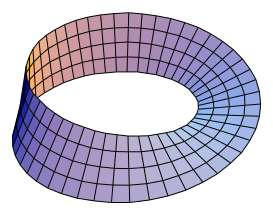
\includegraphics[width=0.35\linewidth]{images/MobiusStrip.pdf}
   \caption[Relationship between Mobius strip and a cylinder]{(\textit{First row}) Flat view of a Mobius strip and a cylinder. (\textit{Second row}) three-dimensional view of a Mobius strip. Images taken from \cite{Kosniowski} and Wikipedia}
   \label{fig:MobiusCylinder}
\end{figure}

At this point, we have seen the main definitions for topology and different ways to generate topological spaces. In the next subsections we will study some interesting topological spaces which will be used in later parts

\subsection{Chain complexes}

Now we can introduce a very important construct of the algebraic topology the \textbf{chain complexes}. They are algebraic means of representing the relationships between \textit{cycles} and \textit{boundaries} in various dimensions of a topological space. To fully understand the theory behind chain complexes we should introduce other interesting definitions first:

\begin{definition}[Standard n-simplex]
 The \textbf{standard n-simplex} $\Delta_{n}$ is defined to be the following subspace of $\mathbb{R}^{n+1}$:\\
 $\Delta_{n} = \{ x=(x_{0},x_{1},\dots,x_{n}) \in \mathbb{R}^{n+1}; \displaystyle\sum_{i=0}^{n} x_{i} = 1, x_{i} \geq 0, i = 0,1,\dots,n \}$\\
 The points $v_{0} = (1,0,\dots,0), v_{1} = (0,1,0,\dots,0),\dots, v_{n} = (0,0,\dots,0,1)$ are called the vertices of $\Delta_{n}$
\end{definition}

\begin{figure}[htb] %  figure placement: here, top, bottom
   \centering
   \includegraphics[width=0.80\linewidth]{images/standardSimplices.pdf}
   \caption[Examples of standard n-simplices]{Examples of standard simplices. $\Delta_{0}$ is a point, $\Delta_{1}$ is a line, $\Delta_{2}$ is a triangle and $\Delta_{3}$ is a tetrahedron}
   \label{fig:standardSimplex}
\end{figure}

\begin{definition}[Singular n-simplex]
 Let $X$ be a topological space. A \textbf{singular n-simplex} in $X$ is a continuous map $\varphi \colon \Delta_{n} \rightarrow X$
\end{definition}

So a singular 0-simplex is a point in $X$, while a singular 1-simplex is a path in $X$.

\begin{figure}[htb] %  figure placement: here, top, bottom
   \centering
   \includegraphics[width=0.35\linewidth]{images/singularsimplex.pdf}
   \caption[A singular n-simplex]{A singular n-simplex.}
   \label{fig:singularSimplex}
\end{figure}


Now we can define the \textbf{singular n-chain}:

\begin{definition}[Singular n-chain]
 A singular n-chain in $X$ is an expression of the form $\displaystyle\sum_{j  \in J} n_{j} \varphi_{j}$ where $\{ \varphi_{j}; j \in J \}$ is the collection of all singular n-simplexes in $X$ (with $J$ some indexing set) and $n_{j} \in \mathbb{Z}$ with only a finite number of $\{ n_{j}; j \in J \}$ being non-zero
\end{definition}

In other words we can say that a simplicial k-chain is a linear combination of k-simplices.
The set $S_{n}(X)$ of singular n-chains in $X$ form an abelian group\footnote{We say that an abelian group is a group where its binary operation is commutative} with the addition defined by $\sum n_{j} \varphi_{j} + \sum m_{j} \varphi_{j} = \sum(n_{j} + m_{j}) \varphi_{j}$. This group has extremely interesting properties which we will exploit in the following parts and that makes it a fundamental construct for LAR library.

Now that we have a definition of a chain complex, we can also define the \textbf{cochain complex}:

\begin{definition}[Singular n-cochain]
Given a topological space $X$ and an abelian group $G$, we define the group $C^{n}(X;G)$ of \textbf{singular n-cochains with coefficients in G} to be the dual group of the singular chain group $C_{n}(X)$. Thus an n-cochain $\varphi \in C^{n}(X;G)$ assigns to each singular n-simplex $\sigma \colon \Delta_{n} \rightarrow X$ a value $\varphi(\sigma) \in G$. Since the singular n-simplices form a basis for $C_{n}(X)$, these values can be chosen arbitrarily hence n-cochains are exactly equivalent to functions from singular n-simplices to $G$.
\end{definition}

This definition is taken from~\cite{Hatcher}.
From a computer science point of view, cochains offer a mechanism for representation of quantities associated with combinatorial and discrete representations. As a consequence, we can use them to represent physical properties for our domain.


\subsection{Cell complexes}

Another fundamental construct of algebraic topology, are \textbf{cell complexes}, which provide a useful procedure for the construction of a topological space. As we can see in~\cite{Hatcher} we can use the following procedure:
\begin{enumerate}
 \item Start with a discrete set $X^{0}$, whose points are referred to as \textbf{0-cells}
 \item Inductively, form the \textbf{n-skeleton} $X^{n}$ from $X^{n - 1}$ by attaching n-cells $e^{n}_{\alpha}$ via maps $\varphi_{\alpha} \colon S^{n-1} \rightarrow X^{n-1}$. This means that $X^{n}$ is the quotient space of the disjoint union $X^{n-1} \coprod_{\alpha}D^{n}_{\alpha}$ of $X^{n-1}$ with a collection of n-disks $D^{n}_{\alpha}$ under the identifications $x \sim  \varphi_{\alpha}(x)$ for $x \in \partial D^{n}_{\alpha}$\footnote{$\partial D^{n}_{\alpha}$ is the boundary of the n-disk as we will see in section~\ref{sec21:topologicalOperators}}. Thus as a set, $X^{n} = X^{n-1}\coprod_{\alpha}e^{n}_{\alpha}$ is an open-disk.
 \item One can either stop this inductive process at a finite stage, setting $X = X^{n}$ for some $x < \infty$, or one can continue indefinitely, setting $X = \bigcup_{n}X^{n}$. In the latter case $X$ is given the \textbf{weak topology}: A set $A \subset X$ is open (or closed) iff $A \cap X^{n}$ is open (or closed) in $X^{n}$ for each $n$
\end{enumerate}

A space $X$ constructed in this way is called a \textbf{cell complex} or \textbf{CW complex}. If $X = X^{n}$ for some $n$, then $X$ is said to be finite-dimensional, and the smallest such $n$ is the \textbf{dimension} of $X$, the maximum dimension of cells of X. We could prove that a n-dimensional cell is homeomorphic to a \textit{n-dimensional ball}\\

In addition, \cite{Hatcher} gives us interesting examples of cell complexes. For example a 1-dimensional cell complex $X = X^{1}$ is a \textbf{graph} in algebraic topology. It consists of vertices (the 0-cells) to which edges (the 1-cells) are attached. The two ends of an edge can be attached to the same vertex.\\
Another example consists in considering the sphere $S^{n}$ which is a cell complex with just two cells. These cells are $e^{0}$ and $e^{n}$, where the n-cell is attached by the constant map $S^{n-1} \rightarrow e^{0}$. This is equivalent to considering $S^{n}$ as the quotient space $D^{n}/\partial D^{n}$.\\

We can also give the following definition:

\begin{definition}[Subcomplex]
A \textbf{subcomplex} of a cell complex $X$ is a closed subspace $A \subset X$ that is a union of cells of $X$. Since $A$ is closed, the characteristic map of each cell in $A$ has image contained in $A$, and in particular the image of the attaching map of each cell in $A$ is contained in $A$, so $A$ is a cell complex in its own right. A pair $(X,A)$ consisting of a cell complex $X$ and a subcomplex $A$ will be called a \textbf{CW pair}.
\end{definition}

According to \cite{Hatcher}, we can also define various operations on cell complexes. We have:
\begin{description}
 \item \textbf{Products}. If $X$ and $Y$ are cell complexes, then $X \times Y$ has the structure of a cell complex where cells are the products $e^{m}_{\alpha} \times e^{n}_{\beta}$ where $e^{m}_{\alpha}$ ranges over the cells of $X$ and $e^{n}_{\beta}$ over the cells of $Y$
 \item \textbf{Quotients}.  If $(X, A)$ is a CW pair consisting of a cell complex $X$ and a subcomplex $A$, then the quotient space $X/A$ inherits a cell complex structure from $X$. The cells of $X/A$ are the cells of $X - A$ plus one new 0-cell, which is the image of $A$ in $X/A$. For a cell $e^{n}_{\alpha}$ of $X-A$ attached by $\varphi_{\alpha} \colon S^{n-1} \rightarrow X^{n-1}$, the attaching map for the corresponding cell in $X/A$ is the composition $S^{n-1} \rightarrow X^{n-1} \rightarrow X^{n-1}/A^{n-1}$
 \item \textbf{Suspension}. For a space $X$, the suspension $SX$ is the quotient of $X \times I$ obtained by collapsing $X \times \{0\}$ to one point and $X \times \{1\}$ to another point.
 \item \textbf{Join}. Given $X$ and a second space $Y$, one can define the space of all line segments joining points in $X$ to points in $Y$. This is the join $X \ast Y$, the quotient space of $X \times Y \times I$ under the identifications $(x, y_{1}, 0) \sim (x, y_{2}, 0)$ and $(x_{1}, y, 1) \sim (x_{2}, y, 1)$. Thus we are collapsing the subspace $X \times Y \times \{0\}$ to $X$ and $X \times Y \times \{1\}$ to $Y$.
 \item \textbf{Wedge Sum}. Given spaces $X$ and $Y$ with chosen points $x_{0} \in X$ and $y_{0} \in Y$, then the wedge sum $X \vee Y$ is the quotient of the disjoint union $X \sqcup Y$ obtained by identifying $x_{0}$ and $y_{0}$ to a single point.
 \item \textbf{Smash Product}. Inside a product space $X \times Y$ there are copies of $X$ and $Y$, namely $X \times \{y_{0}\}$ and $\{x_{0}\} \times Y$ for points $x_{0} \in X$ and $y_{0} \in Y$. These two copies of $X$ and $Y$ in $X \times Y$ intersect only at the point $(x_{0}, y_{0})$, so their union can be identified with the wedge sum $X \vee Y$. The smash product $X \wedge Y$ is then defined to be the quotient $X \times Y/X \vee Y$
\end{description}
In Figure~\ref{fig:cellOperations} there is a graphical representation of all these operations.

\begin{figure}[htbp] %  figure placement: here, top, bottom
   \centering
   (a)\includegraphics[width=0.50\linewidth]{images/productTopology.jpg}\hfill
   (b)\includegraphics[width=0.23\linewidth]{images/quotientTopology.pdf}\hfill
   (c)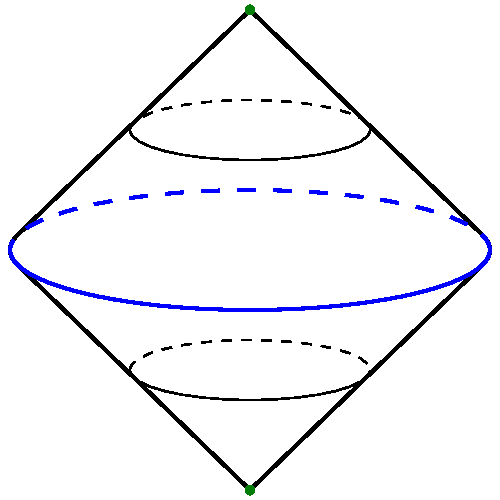
\includegraphics[width=0.30\linewidth]{images/suspensionTopology.pdf}\\
   (d)\includegraphics[width=0.30\linewidth]{images/joinTopology.pdf}\hfill
   (e)\includegraphics[width=0.30\linewidth]{images/wedgeSum.pdf}\\
   (f)\includegraphics[width=0.30\linewidth]{images/smashProduct.png}\\
   \caption[Operations on cell complexes]{Operations on cell complexes.\\ (a) A product topology. How we can see, a cylinder can be obtained with a product between a circle and a line. Image taken from \href{http://scienceblogs.com/goodmath/2006/09/21/topological-products/}{scienceblogs.com}\\ (b) A quotient topology. Intuitively we have a quotient topology when we glue spaces points together. For example we can obtain a torus by gluing opposite sides of a square. Image taken from \href{http://mathroughguides.wikidot.com/article:point-set-topology}{mathroughguides.wikidot.com}\\ (c) A suspension topology. The original space is in blue and the collapsed end points are in green. Image taken from Wikipedia.\\ (d) Geometric join of two line segments. The original spaces are in blue and green. The join is a three-dimensional solid in black. Image taken from Wikipedia\\ (e) A wedge sum topology obtained by attaching two circumferences by a point\\ (f) Smash product. In this example we build a smash product starting from two segments. The product topology produces a square and then the vertical and the horizontal lines are collapsed to a point. Image taken from \href{http://www.math.ntnu.no/~stacey/Seminars/chern.html}{www.math.ntnu.no}}
   \label{fig:cellOperations}
\end{figure}

\section{LAR representation schema}\label{sec21:LAR}

As stated in \cite{DiCarlo} (and also in the first chapters of this work), present-day computational problems in science and technology must deal with increasingly complex geometric information. The evolution of 3D geometric representations can be generally understood in terms of graph-based data structures representing one of several possible cell complexes partitioning either the boundary or the interior of the represented model. However, we can make a lot of assumptions about cell complexes and graph representations, so standardization seem difficult to reach. Thus the specialized data structures that have been used since now, are no longer adequate to deal with these problems.\\

\cite{DiCarlo} provides a solution to these problems with a new representation schema which supports all topological constructions and queries useful in typical cellular decomposition of space: \textbf{LAR}. Formally, LAR uses the standard definitions of the mod-2 cell complexes. So we have \textit{n-chains} which are sets of \textit{n-cells}. The standard basis of the $\mathbb{Z}_{2}$-linear space $C_{d}$ of n-chains is provided by singletons of n-cells; each n-cell is represented by a map $C_{n} \rightarrow \mathbb{Z}_{2}C_{0}$, i.e. by a row of a binary characteristic matrix $M_{n}$. Obviously, each n-chain in $C_{n}$ can be generated by a $(\mathbb{Z}_{2})$-linear combination of $M_{n}$ rows. This formulation can be extended to n-cochains that represent any possible field over the chains.\\

\begin{figure}[htb] %  figure placement: here, top, bottom
   \centering
   \includegraphics[width=0.75\linewidth]{images/larcomplex.pdf}\\
   \includegraphics[width=0.85\linewidth]{images/larRepresentation.png}
   \caption[LAR representation schema]{LAR representation schema. We can see the relationship between chains of different dimensions and how to represent them using a characteristic matrix. Images taken from \cite{DiCarlo}}
   \label{fig:larRepresentation}
\end{figure}

Figure~\ref{fig:larRepresentation}, points out that characteristic matrices are very sparse for actual chain complexes, so they can be represented in the \textbf{Compressed Sparse Row} (CSR) format in order to save space. This format is widely used in computer science, and consists in using three one-dimensional arrays. The first one save the non-zero values as they are traversed in a row-wise fashion, while the second stores the columns indices of the values. The last one stores the locations of the values array that start a row. Moreover, if we have a binary matrix we can safely delete the first array, as the non-zero value can only be $1$. In addition this data structure is faster than a traditional one, because the \textbf{sparse matrix-vector multiplication} (SpMV) is linear in the size of the output.\\

Now we can deeply study the LAR representation from a formal point of view using concepts from \cite{DiCarlo}. First of all we need to consider a cellular complex $\Lambda(X)$ such that $X = \Lambda_{0} \cup \dots \cup \Lambda_{d}$. We can define $M_{p} \in \mathbb{Z}_{2}^{m\times n} (0\leq p \leq d)$ as the characteristic matrices, with number of rows equal to the number of p-cells and number of columns equal to the number of 0-cells:
\begin{equation}
 m = k_{p} = \#\Lambda_{p}, \; \; \; \; \; \; \; \; n = k_{0} = \#\Lambda_{0}
\end{equation}

Each $m_{ij} \in M_{p}$ tells us whether the vertex $v_{j} \in \Lambda_{0}$ is contained on the boundary of the cell $\lambda_{i} \in \Lambda_{p}$ or not. So the LAR schema is a map from a mathematical model of a solid to its computer representation:
\begin{equation}
 LAR \colon \mathbb{C}h(\Lambda(X)) \rightarrow (M_{p})^{d}_{p=1}
\end{equation}

So we can have the following definition from \cite{DiCarlo}:
\begin{definition}[LAR representation]
 $LAR$ represents chain complexes $\mathbb{C}h$, supported by a finite cellular complex $\Lambda(X)$, by $d-$tuples of binary CSR matrices, where $d$ is the dimension of the space $X$
\end{definition}

For a cellular $d-$complex $\Lambda(X)$, all the $M_{p}$ matrices have the same number of columns, so we can use standard matrix transposition and multiplication. Thus we can easily compute \textit{boundary} and \textit{coboundary} operators (see Section~\ref{sec21:topologicalOperators}) and topological relations between cells.\\

Summing up, we have seen that this new representation schema, help us define cell complexes in a very simple way.\\

In addition, we can consider a common situation where a topological structure is a regular $d-$complex (so every cell is contained in some $d-$cell). In this case, \cite{DiCarlo} defines a \textbf{reduced LAR representation} under the following assumptions:
\begin{itemize}
 \item LAR contains both the $d-$cells of a regular decomposition of a $d-$space and of its complement
 \item Any two cells intersect on a connected cell
\end{itemize}

In this case the highest dimensional $CSR(M_d)$ matrix is a valid reduced LAR representation in the sense that all lower-dimensional $M_p$ matrices and operators may be computed from the matrix $M_d$. Therefore we can say that $CSR(M_d)$ \textbf{fully characterizes the chain complex}.\\

Another representation (which is defined in \cite{cclar}), is the \textbf{BRC representation}. It is based on arrays of integers, with no requirement of equal length for the component arrays. Each component array corresponds to a matrix row and contains the indices of columns that store a 1 value. In \cite{cclar} we can find the following example:
\[
A = \begin{pmatrix}
0 & 1 & 0 & 0 & 0 & 0 & 0 & 1 & 0 & 0\\
0 & 0 & 1 & 0 & 0 & 0 & 0 & 0 & 0 & 0\\
1 & 0 & 0 & 1 & 0 & 0 & 0 & 0 & 0 & 1\\
1 & 0 & 0 & 0 & 0 & 0 & 1 & 0 & 0 & 0\\
0 & 0 & 0 & 0 & 0 & 1 & 1 & 1 & 0 & 0\\
0 & 0 & 1 & 0 & 1 & 0 & 0 & 0 & 1 & 0\\
0 & 0 & 0 & 0 & 0 & 0 & 0 & 0 & 0 & 0\\
0 & 1 & 0 & 0 & 0 & 0 & 0 & 1 & 0 & 1\\
0 & 0 & 0 & 1 & 0 & 0 & 0 & 0 & 1 & 0\\
0 & 1 & 1 & 0 & 1 & 0 & 0 & 0 & 0 & 0\\
\end{pmatrix}
\quad\mapsto\quad \texttt{BRC}(A) =
\begin{minipage}[c]{5cm}
\begin{verbatim}
[[1,7],
 [2],
 [0,3,9],
 [0,6],
 [5,6,7],
 [2,4,8],
 [],
 [1,7,9],
 [3,8],
 [1,2,4]]
\end{verbatim}
\end{minipage}
\]

In the next section we will see how to define topological operators in order to manipulate them.

\section{Some interesting topological operators}\label{sec21:topologicalOperators}

Now we can define some interesting operators for manipulation of our topological structures. First of all we are interested in incidence queries that arise in a cellular decomposition $\Lambda(X)$ of a two-dimensional space. We can have nine relations:

\begin{table}[htbp]
\centering
\caption[Incidence queries]{Incidence queries}
\label{tbl:incidence}
\begin{tabular}{ccc}
$VV \colon C_{0} \rightarrow C_{0}$	&$EV \colon C_{0} \rightarrow C_{1}$	&$FV \colon C_{0} \rightarrow C_{2}$\\ 
$VE \colon C_{1} \rightarrow C_{0}$	&$EE \colon C_{1} \rightarrow C_{1}$	&$FE \colon C_{1} \rightarrow C_{2}$\\
$VF \colon C_{2} \rightarrow C_{0}$	&$EF \colon C_{2} \rightarrow C_{1}$	&$FF \colon C_{2} \rightarrow C_{2}$\\
\end{tabular}
\end{table}

As we can see in \cite{DiCarlo}, with LAR we can compute these relations with only SpMV multiplications:
\begin{description}
 \item $VV = VE \circ EV = EV^{\mathsf{T}} \circ EV \Rightarrow [VV] = M_{1}^{\mathsf{T}}M_{1}$
 \item $VE = EV^{\mathsf{T}} \Rightarrow [VE] = M_{1}^{\mathsf{T}}$ 
 \item $VF = FV^{\mathsf{T}} \Rightarrow [VF] = M_{2}^{\mathsf{T}}$ 
 \item $EV [VV] = M_{1}$ 
 \item $EE = EV \circ VE = EV \circ EV^{\mathsf{T}} \Rightarrow [EE] = M_{1}M_{1}^{\mathsf{T}}$ 
 \item $EF = EV \circ VF = EV \circ FV^{\mathsf{T}} \Rightarrow [EF] = M_{1}M_{2}^{\mathsf{T}}$ 
 \item $FV [FV] = M_{2}$ 
 \item $FE = FV \circ VE = FV \circ EV^{\mathsf{T}} \Rightarrow [FE] = M_{2}M_{1}^{\mathsf{T}}$ 
 \item $FF = FV \circ VF = FV \circ FV^{\mathsf{T}} \Rightarrow [FF] = M_{2}M_{2}^{\mathsf{T}}$ 
\end{description}

Now we will study one of the most important operators in topological algebra: the \textbf{boundary operator}. Intuitively, a boundary of a subset $S$ of a topological space $X$ is the set of points which can be approached both from $S$ and from the outside of $S$. So it is a set of points that belong to $S$ but do not belong to its interior. Thus using the boundary operator we are able to pass from a $d-$dimensional chain to a $(d-1)-$dimensional one. \cite{Kosniowski} gives us a good definition of the boundary operator:

\begin{definition}[Boundary operator]
 The \textbf{boundary operator} $\partial \colon S_{d}(X) \rightarrow S_{d-1}(X)$ is defined by:\\
 $\partial = \partial_{0} - \partial_{1} + \partial_{2} - \dots + (-1)^{d}\partial_{d} = \displaystyle\sum_{i=0}^{d} (-1)^i\partial_{i}$
\end{definition}

This leads to the definition of two interesting subgroups of $S_{d}(X)$:

\begin{definition}[Cycles]
 A singular $d-$chain $c \in S_{d}(X)$ is a \textbf{$\mathbf{d-}$cycle} if $\partial_{c} = 0$. The set of $d-$cycles in $X$ is denoted by $Z_{d}(X)$
\end{definition}
 
\begin{definition}[d-boundaries]
 A singular $d-$chain $b \in S_{d}(X)$ is a \textbf{$\mathbf{d-}$boundary} if $b = \partial_{e}$ for some $e \in S_{d+1}(X)$. The set of $d-$boundaries in $X$ is denoted by $B_{n}(X)$
\end{definition}

We can also define the \textbf{coboundary operator} ($\delta^{d}$) on cochains as the dual of the boundary operator whereby we can pass from a $(d-1)-$dimensional complex to a $d-$dimensional one. In Figure~\ref{fig:larComplexMap} there is a representation of the relationships between chains and cochains of different dimensions:

\begin{figure}[htb] %  figure placement: here, top, bottom
   \centering
   \includegraphics[width=0.75\linewidth]{images/chainComplexMap.png}\\
   \caption[Relationships between chains and cochains]{Relationships between chains and cochains}
   \label{fig:larComplexMap}
\end{figure}

At this point we are interested in computing these operators in an efficient way. As always, \cite{DiCarlo} provides an interesting algorithm based on the LAR representation schema. First of all, we should consider the incidence map $\ell_{p-1}^{p} \colon C_{p} \rightarrow C_{p-1}$ and its matrix $[\ell_{p-1}^{p}] = M^{p}_{p-1} = M_{p-1}M^{\mathsf{T}}_{p}$. The entry $M_{p-1}^{p}[i,j]$ stores the number $k$ of common vertices between the cells $\mu_{p-1}^{i}$ and $\lambda_{p}^{j}$, where $\mu \in \Lambda_{d-1}$ is the common facet between cell complexes and $\lambda \in \Lambda_{d}$ represents a single cell. In fact we have: $M^{p}_{p-1}[i,j] = \displaystyle\sum_{h=0}^{k_{0}-1} M_{p-1}[i,h] \cdot M_{p}[j,h] = \# (\mu_{p-1}^{i} \cap \lambda_{p}^{j}) = k$. So if we want to compute the \textbf{unoriented boundary} operator, we can use the following algorithm:

\begin{pseudo}[caption={Unoriented boundary algorithm}, label={lst:Boundary}]
begin
 $CSR(M_{p-1}^{p}) = CSR(M_{p-1})CSR(M_{p}^{\mathsf{T}})$
 foreach $i$ in $0 \leq i \leq k_{p-1} - 1$:
   $k = \#\mu_{p-1}^{i}$ //Number of nonzero elements for row $i$ of $CSR(M_{p-1})$
   foreach $j$ in $0 \leq j \leq k_{p} - 1$:
     if $M^{p}_{p-1}[i,j] = k$:
       $\partial_{p}[i, j] = 1$
     else:
       $\partial_{p}[i, j] = 0$
 return $\partial_{p}$
end       
\end{pseudo}

By duality, we can obtain the coboundary operator as the transposition of $\partial_{p}$ operator. For a better understanding of this algorithm we can see an example of $\partial_{2}$ computation from \cite{DiCarlo}. First of all we have to consider the cell complex in Figure~\ref{fig:boundaryExample} with the characteristic matrices $M_1$ and $M_2$.

\begin{figure}[htb] %  figure placement: here, top, bottom
   \centering
   \includegraphics[width=0.35\linewidth]{images/boundaryExample.png}\\
   \caption[Cuboidal complex]{Cuboidal complex. Image taken from \cite{DiCarlo}}
   \label{fig:boundaryExample}
\end{figure}

According to the algorithm we have that $M_{1}^{2} = M_{1}M_{2}^{\mathsf{T}}$. So if:\\

$M_2 =
\begin{pmatrix}
1 & 1 & 0 & 0 & 0 & 0 & 1 & 1\\
1 & 0 & 1 & 0 & 1 & 0 & 1 & 0\\
0 & 0 & 0 & 0 & 1 & 1 & 1 & 1\\
0 & 1 & 0 & 1 & 0 & 1 & 0 & 1\\
0 & 0 & 1 & 1 & 1 & 1 & 0 & 0\\
1 & 1 & 1 & 1 & 0 & 0 & 0 & 0\\
\end{pmatrix}
M_1 =
\begin{pmatrix}
1 & 1 & 0 & 0 & 0 & 0 & 0 & 0\\
1 & 0 & 1 & 0 & 0 & 0 & 0 & 0\\
1 & 0 & 0 & 0 & 0 & 0 & 1 & 0\\
0 & 1 & 0 & 1 & 0 & 0 & 0 & 0\\
0 & 1 & 0 & 0 & 0 & 0 & 0 & 1\\
0 & 0 & 1 & 1 & 0 & 0 & 0 & 0\\
0 & 0 & 1 & 0 & 1 & 0 & 0 & 0\\
0 & 0 & 0 & 1 & 0 & 1 & 0 & 0\\
0 & 0 & 0 & 0 & 1 & 1 & 0 & 0\\
0 & 0 & 0 & 0 & 1 & 0 & 1 & 0\\
0 & 0 & 0 & 0 & 0 & 1 & 0 & 1\\
0 & 0 & 0 & 0 & 0 & 0 & 1 & 1\\
\end{pmatrix}$

we can obtain:\\

$M^{2}_{1} =
\begin{pmatrix}
2 & 1 & 0 & 1 & 0 & 2\\
1 & 2 & 0 & 0 & 1 & 2\\
2 & 2 & 1 & 0 & 0 & 1\\
1 & 0 & 0 & 2 & 1 & 2\\
2 & 0 & 1 & 2 & 0 & 1\\
0 & 1 & 0 & 1 & 2 & 2\\
0 & 2 & 1 & 0 & 2 & 1\\
0 & 0 & 1 & 2 & 2 & 1\\
0 & 1 & 2 & 1 & 2 & 0\\
1 & 2 & 2 & 0 & 1 & 0\\
1 & 0 & 2 & 2 & 1 & 0\\
2 & 1 & 2 & 1 & 0 & 0\\
\end{pmatrix}
\Rightarrow \partial_{2} = 
\begin{pmatrix}
1 & 0 & 0 & 0 & 0 & 1\\
0 & 1 & 0 & 0 & 0 & 1\\
1 & 1 & 0 & 0 & 0 & 0\\
0 & 0 & 0 & 1 & 0 & 1\\
1 & 0 & 0 & 1 & 0 & 0\\
0 & 0 & 0 & 0 & 1 & 1\\
0 & 1 & 0 & 0 & 1 & 0\\
0 & 0 & 0 & 1 & 1 & 0\\
0 & 0 & 1 & 0 & 1 & 0\\
0 & 1 & 1 & 0 & 0 & 0\\
0 & 0 & 1 & 1 & 0 & 0\\
1 & 0 & 1 & 0 & 0 & 0\\
\end{pmatrix}$
\chapter{Mastering big data using parallel computing}\label{Chapter22} % Main chapter title
\thispagestyle{empty}
Usually we design our softwares thinking that they will run on a single \textit{executor}. However the increase of data sizes, and the consequent needs for architectures that can do efficient computations, determined the birth of a new programming model: \textbf{parallel computing}. The main idea at the basis of this model is that if a single computer is not able to compute operations on a huge quantity of data, so we can connect more and more computers in \textit{parallel} to get our computation done. Indeed, by now we have parallelism at several levels of our architectures. For example modern CPUs are designed with the aim of executing parallel code and also GPUs can be used for this purpose. However, in this work we are mainly focused on \textbf{clusters} of supercomputers, as we will see in detail in Section~\ref{sec22:parallelArchitectures}. In this chapter we will also study one of the most important tools for parallel computing: MPI

\section{Principles of parallel computing}\label{sec22:parallelComputing}

As we have seen in previous chapters, big data are deeply changing computer science and all its branches. So to deal with this new challenge we need to rethink our programming models and, how we have read in the introduction to this chapter, \textbf{parallel computing} can be an answer to these requests. According to \cite{Eijkhout}, parallel computing is simply an answer to the following problem: if there are $n$ operations to be done ans they would take time $t$ on a single processor, can they be done in time $t/p$ on $p$ processors?.\\

We use a parallel computer for two important reasons: to \textit{have access to more memory} and to \textit{obtain higher performance}. While it is simple to understand the gain in memory, as the total memory is the sum of the individual memories, the speed is harder to characterize. First of all we can give the following definition:

\begin{definition}[Speedup]
 Given $T_{1}$ as the best time to solve a problem in a single processor, and $T_{p}$ as the best solving time for the same problem with $p$ processors, we define the \textbf{speedup} $S_{p}$ as: $S_{p} = \frac{T_{1}}{T_{p}}$. 
\end{definition}

As we can see in the definition, we usually use different algorithms on different architectures in order to obtain the most efficient code possible. In the ideal case, $T_{p} = \frac{T_{1}}{p}$ (\textbf{perfect speedup}) but in practice is very difficult to obtain it, so $S_{p} \leq p$. To measure how far we are from the ideal speedup we can introduce the \textbf{efficiency} as $E_{p} = \frac{S_{p}}{p}$. As we can see $0 < E_{p} \leq 1$.\\

One of the reasons why we do not have perfect speedup, is that parts of a code can be inherently sequential. Supposing that 5\% of a code is sequential, then the time for that part cannot be reduced. Thus the speedup on that code is limited to a factor of 20. This phenomenon is described by the \textbf{Amdahl's Law}. According to \cite{Eijkhout} we can use the following definition:

\begin{definition}[Amdahl's law]
 Let $F_{s}$ be the sequential fraction and $F_{p}$ be the parallel fraction of a code. Then $F_{p} + F_{s} = 1$. The parallel execution time $T_{p}$ on $p$ processors is the sum of the part that is sequential ($T_{1}F_{s}$) and the part that can be parallelized ($T_{1}\frac{F_{p}}{p}$):
 \begin{equation}
  T_{p} = T_{1}(F_{s} + \frac{F_{p}}{p})
 \end{equation}
\end{definition}

When we have $p \rightarrow \infty$, the parallel execution time tends to $T_{1}F_{s}$, so the upper bound for the speedup is $S_{p} \leq \frac{1}{F_{s}}$.

\begin{figure}[htb] %  figure placement: here, top, bottom
   \centering
   \includegraphics[width=0.70\linewidth]{images/AmdahlsLaw.pdf}\\
   \caption[Amdahl's Law]{Amdahl's Law. Image taken from Wikipedia}
   \label{fig:AmdahlsLaw}
\end{figure}

Amdahl's law is optimistic. In fact code parallelization give a speedup, but it also introduces communication overhead between processes. So if $T_{c}$ is the time spent on communication, we have:
\begin{equation}
 T_{p} = T_{1}(F_{s} + \frac{F_{p}}{p}) +  T_{c}
\end{equation}

Assuming we have a fully parallelized code, we can write:
\begin{equation}
 S_{p} = \frac{T_{1}}{T_{1}/p + T_{c}}
\end{equation}

Thus, to be close to $p$ we need $T_{c} \ll T_{1}/p$ or $p \ll T_{1}/T_{c}$.\\

As a consequence of the Amdahl's Law, our speedup is limited, so we do not have a great improvement with large-scale supercomputers. So now we are wondering why we should use parallel computing. In fact, when dealing with big data, we are not only interested in speedup but also in \textit{memory gain}. So, using this technique we are sure that our algorithms can finish returning a result. In this work, a primary importance is given to the improvement of memory occupation, as the three-dimensional models that we will create can be huge.

\section{Typical architectures for parallel computing}\label{sec22:parallelArchitectures}

Now we are interested in studying the most common architectures for parallel computing. A good source for this argument is \cite{Matloff}. How we can see there, these architectures are commonly divided into two groups: \textbf{shared-memory systems} and \textbf{message-passing systems}

\subsection{Shared-memory systems}

With this architecture, many CPUs share the same physical memory. So we talk about \textbf{MIMD}, which stands for \textit{Multiple Instruction Multiple Data}. In fact we have many different independent CPUs which access different memory locations at any given time. In these days, shared-memory systems are very common even on consumer PCs and mobile phones.\\

As an example we can consider a program which has a global variable $X$ and a local variable $Y$ on this hardware. If the compiler assigns location $200$ to $X$, then all processors will have that variable in common. In fact, any processor which issues a memory operation on location $200$ will access the \textit{same physical memory cell}. On the other hand, each processor will have its own run-time stack. All stacks are in shared memory, but they are accessed separately as each CPU has a different value in its stack pointer. Thus each processor will have its own independent copy of the local variable $Y$.\\

From a parallel point of view, each execution of a program requires parallel accessing of memory in order to avoid slowdowns. In parts this is handled by having a cache at each CPU, but it is also facilitated by dividing the memory into separate modules or \textit{banks}. The division can be done with two main strategies:
\begin{itemize}
 \item \textbf{High-order interleaving}: consecutive words are in the same bank (except at boundaries). It is widely used when dealing with matrices.
 \item \textbf{Low-order interleaving}: consecutive addresses are in consecutive banks (except when we get to the right end). It is widely used in GPUs
\end{itemize}

For a better understanding of shared-memory systems we can do the following example. Suppose we have to implement a matrix-vector multiplication between a vector $X$ and a matrix $A$ producing vector $Y$. The arrays for $A$, $X$ and $Y$ are held in common by all nodes. Then, each node multiply its assigned rows of $A$ times $X$ and place the result directly in the proper section of $Y$. From a technical point of view, these operations are usually done with \textit{threads}.

\subsection{Message-passing systems}

In message-passing systems, we have a certain number of independent CPUs each with its own independent memory. All processors communicate using some kind of network protocol. A typical environment for these systems is a \textbf{cluster} of different PCs. The idea consists in taking several PCs and networks and divide the computation sending \textbf{messages} to them containing their part of input data. Obviously, we need a fast network to avoid slowdowns due to network communication. The common choice today is \textit{Infiniband} as the traditional TCP/IP networks are quite slow. The common paradigm used in message-passing systems is the \textbf{scatter/gather paradigm}. According to this paradigm, we have a \textit{manager} node which sends out chunks of work to the other nodes, which are called \textit{workers}. When they have finished their work, workers send back to the manager the results which will be collected and assembled.\\

Now we can consider the same example as above of matrix-vector multiplication. With this architecture one node (for example node $0$) distributes the rows of $A$ to the other ones, so that each node receive a different set of rows, and the vector $X$ to all nodes. Each node then multiply $X$ by its own assigned rows of $A$ and then send back the results to node $0$ which will collect all parts and store in $Y$ the final result\\

As this type of architecture is the one chosen for our software, we will describe it more deeply when we will see the most important technology for implementation of a message-passing system: MPI.

\section{The Message Passing Interface}\label{sec22:MPI}

According to \cite{Matloff}, the \textbf{message-passing interface} or \textbf{MPI}, is a set of API called from user programs which provides a communication protocol for message-passing systems. So it is able to abstract all communications between processes. In MPI abstraction, when we write a program which will be run on four machines of the clusters, every machine  executes its own copy of the program and following official terminology we say we have four \textbf{processes}. Though the nodes are all running the same program, they will likely be working on different parts of its data. This is called the \textbf{Single Program Multiple Data} (\textbf{SPMD}).\\

From an architectural point of view, one of the most important parts of MPI is the \textbf{communicator}. It connects group of processes in the MPI session giving to each one an independent identifier which is called \textbf{rank}. By default the rank 0 process belongs to the MPI process that starts the program. Moreover the communicator arranges these processes in an ordered topology.\\

MPI also provides powerful methods for \textbf{point to point communications}. An example is \texttt{MPI\_Send} function, which allows one process to send a message to a second process. These type of communications are useful in irregular communication (for example a master-slave architecture where the master sends new data task to a slave whenever the prior task is completed).\\

Moreover MPI provides functions for \textbf{collective communications}:
\begin{itemize}
 \item \texttt{MPI\_Bcast}: The root sends messages from a buffer to all other processes
 \item \texttt{MPI\_Scatter}: The root has a buffer message and splits it into $n$ parts (where $n$ is the number of processes), then send each part to the corresponding process.
 \item \texttt{MPI\_Gather}: It is the opposite of scatter, in fact the root fills a buffer concatenating $n$ messages
 \item \texttt{MPI\_Reduce}: As in the gather function the root fills the buffer with $n$ messages. However, the collected data is then "reduced" using an associative function and the function returns the resulting value-
\end{itemize}



\chapter{The Julia language}\label{Chapter23} % Main chapter title
\thispagestyle{empty}
In this work has been used the \textbf{Julia language} as the main programming language. As we can see from its website\footnote{http://julialang.org/}, it is a high-level and high-performance language for technical computing, with a syntax that is well known for everybody uses scientific programming languages. It also provides a compiler, distributed parallel execution and a mathematical function library. We chose it because of these characteristics and because it permits to parallelize programs in a very simple way.\\

In next sections we will see in detail its characteristics and the code used for parallel computation.

\section{Principal characteristics}\label{sec23:julia}
As we can see in the Julia website, this language has the following characteristics:
\begin{itemize}
 \item Multiple dispatch: providing ability to define function behavior across many combinations of argument types
 \item Dynamic type system: types for documentation, optimization, and dispatch
 \item Good performance, approaching that of statically-compiled languages like C
 \item Built-in package manager
 \item Lisp-like macros and other metaprogramming facilities
 \item Call Python functions: use the PyCall package
 \item Call C functions directly: no wrappers or special APIs
 \item Powerful shell-like capabilities for managing other processes
 \item Designed for parallelism and distributed computation
 \item Coroutines: lightweight “green” threading
 \item User-defined types are as fast and compact as built-ins
 \item Automatic generation of efficient, specialized code for different argument types
 \item Elegant and extensible conversions and promotions for numeric and other types
 \item Efficient support for Unicode, including but not limited to UTF-8
 \item MIT licensed: free and open source
\end{itemize}

From the syntax point of view, Julia takes inspiration from various dialects of \textit{Lisp}, including \textit{Scheme} and \textit{Common Lisp}, and it shares many features with \textit{Dylan} and \textit{Fortress}. Is is also possible to implement \textbf{metaprogramming} using macros. They are necessary because they are executed when code is parsed, therefore, macros allow the programmer to generate and include fragments of customized code before the full program is run. We can see the difference in the following example taken from the official documentation:

\begin{julia}
 > macro twostep(arg)
     println("I execute at parse time. The argument
             is: ", arg)
     return :(println("I execute at runtime. 
            The argument is: ", $arg))
   end
 
 > ex = macroexpand( :(@twostep :(1, 2, 3)) );
   "I execute at parse time. The argument
      is: :((1,2,3))"
 
 > typeof(ex)
   Expr

 > ex
   :(println("I execute at runtime. The argument is: 
     ",$(Expr(:copyast, :(:((1,2,3)))))))

 > eval(ex)
   "I execute at runtime. The argument is: (1,2,3)"
\end{julia}

Macro are invoked using the following syntax:
\begin{julia}
 @name expr1 expr2 ...
\end{julia}

In addition, Julia includes an interactive session shell called \textbf{REPL}, which can be used to make experiments and fast code testing. For example we can write:
\begin{julia}
 julia> p(x) = 2x^2 + 1; f(x, y) = 1 + 2p(x)y
 julia> f(0, 4)
 9
\end{julia}

All these commands can also be written in a script file with \texttt{.jl} extension and executed in the shell with:
\begin{julia}
 user@pc: julia <filename>
\end{julia}

As we have seen in the list above Julia has good performances, which are achieved using \textbf{just-in-time (JIT)} compilation, implemented using \textit{LLVM}. This compiler, combined with the language's design allow it to approach the C performances. In table~\ref{tbl:JuliaBenchmark} we can see a little benchmark coming from the official website:

\begin{table}[htb]
\centering
\caption[benchmark times relative to C]{benchmark times relative to C (smaller is better, C performance = 1.0). Table taken from the official documentation}
\label{tbl:JuliaBenchmark}
\begin{tabular}{p{1.2cm} | p{1.2cm} | p{1.3cm} | p{1.3cm} | p{1.3cm} | p{1cm} | p{1cm} | p{1cm}}
\toprule
&\textbf{fib}& \textbf{parse-int}&\textbf{quick-sort}& \textbf{mandel}&\textbf{pi-sum}& \textbf{rand-mat-stat}& \textbf{rand-mat-mul}\\ \midrule
\textbf{Fortran} 	& 0.70	& 5.05	& 1.31	& 0.81	& 1.00	& 1.45	& 3.48\\ \midrule
\textbf{Julia}		& 2.11	& 1.45	& 1.15	& 0.79	& 1.00	& 1.66	& 1.02\\ \midrule
\textbf{Python}         & 77.76	& 17.02	& 32.89	& 15.32	& 21.99	& 17.93	& 1.14\\ \midrule
\textbf{R}		&533.52	& 45.73	&264.54	& 53.16	& 9.56	& 14.56	& 1.57\\ \midrule
\textbf{Matlab}		& 26.89	&802.52	& 4.92	& 7.58	& 1.00	& 14.52	& 1.12\\ \midrule
\textbf{Octave}         &9324.35&9581.44&1866.01&451.81	&299.31	& 30.93	& 1.12\\ \midrule
\textbf{Mathe-matica}	&118.53	&15.02	& 43.23	& 5.13	& 1.69	& 5.95	& 1.30\\ \midrule
\textbf{Java-script}	& 3.36	& 6.06	& 2.70	& 0.66	& 1.01	& 2.30	& 15.07\\ \midrule
\textbf{Go}		& 1.86	& 1.20	& 1.29	& 1.11	& 1.00	& 2.96	& 1.42\\ \midrule
\textbf{LuaJIT}         & 1.71	& 5.77	& 2.03	& 0.67	& 1.00	& 3.27	& 3.27\\ \midrule
\textbf{Java}	        & 1.21	& 3.35	& 2.60	& 1.35	& 1.00	& 3.92	& 2.36\\ \midrule
\bottomrule
\end{tabular}
\end{table}

Julia supports also modular applications. In particular, modules in Julia are separate global variable workspaces. They are delimited by the keywords:
\begin{julia}
 module Name
 ...
 end
\end{julia}

With modules, one can create top-level definitions without worrying about name conflicts. Within a module, it is possible to control which names from other modules are visible (via importing), and specify which names are intended to be public (via exporting). In the official documentation we can find the following example:
\begin{julia}
 module MyModule
 export x, y
 x() = "x"
 y() = "y"
 p() = "p"
end
\end{julia}
In this module we export the x and y functions (with the keyword \texttt{export}), and also have the non-exported function p. In Table~\ref{tbl:juliaImports} there are several different ways to load the Module and its inner functions into the current workspace.

\begin{table}[htb]
\centering
\caption[Modules loading in Julia]{Modules loading in Julia. Table taken from the official documentation}
\label{tbl:juliaImports}
\begin{tabular}{p{5cm} | p{7cm}}
\toprule
\textbf{Import command}			  & \textbf{What is brought into scope}\\ \midrule
\texttt{using MyModule}			  & All exported names (x and y), MyModule.x, MyModule.y and MyModule.p\\ \midrule
\texttt{using MyModule.x, MyModule.p}     & x and p\\ \midrule
\texttt{using MyModule: x, p}          	  & x and p\\ \midrule
\texttt{import MyModule}	          & MyModule.x, MyModule.y and MyModule.p\\ \midrule
\texttt{import MyModule.x, MyModule.p}	  & x and p\\ \midrule
\texttt{import MyModule: x, p}            & x and p\\ \midrule
\texttt{importall MyModule}               & All exported names (x and y)\\ \midrule
\bottomrule
\end{tabular}
\end{table}

Obviously, we can use file scripts for defining multiple modules. Moreover, including the same code in different modules provides mixin-like behavior. One could use this to run the same code with different base definitions, for example testing code by running it with “safe” versions of some operators:
\begin{julia}
module Normal
include("mycode.jl")
end

module Testing
include("safe_operators.jl")
include("mycode.jl")
end
\end{julia}

\section{Parallel programming in Julia}\label{sec23:parallelJulia}

How we have seen in the earlier chapter, modern computer posses more than one CPU and several computers can be combined together in a cluster. Moreover we have seen the big advantages that this type of architecture can give us. For its parallel features, Julia have chosen an environment based on \textit{message passing} (so we have multiple processes which run in separate memory domains). However, the Julia's implementation of message passing is a bit different from other environments such as MPI. In fact communication is generally "one-sided", so the programmer needs to explicitly manage only one process in a two-process operation. In addition these operations do not seems "message send" and "message receive" but resemble higher-level operations like calls to user functions.\\

The most important primitives, are \textbf{remote references} and \textbf{remote calls}. The former is an object that can be used from any process to refer to an object stored on a particular process, while the latter is a request by one process to call a certain function on certain arguments on another process. A remote call returns a remote reference to its result and \textit{return immediately}, while its process proceeds to the next operation. It is possible to wait for a remote call to finish by calling the function \texttt{wait} on its remote reference (or \texttt{fetch} if we are waiting for its value).\\

Now we can examine some useful functions for parallel programming. The simpler function is \texttt{remotecall()}, which takes as parameters the \textit{index of the process that will do the work}, the function that will be invoked and its parameters. It is considered a low-level interface that provides a finer control on the software. However most parallel programming in Julia, does not reference specific processes or the number of processes available. So usually Julia programmers uses the \texttt{@spawn} macro, which operates on an expression and choose where to do the operation. For example we can write:
\begin{julia}
 julia> r = @spawn rand(2,2)
 RemoteRef(1,1,0)

 julia> s = @spawn 1 .+ fetch(r)
 RemoteRef(1,1,1)

 julia> fetch(s)
 1.10824216411304866 1.13798233877923116
 1.12376292706355074 1.18750497916607167
\end{julia}
Note the use of \texttt{1 .+ fetch(r)} instead of \texttt{1 .+ r}. This is because we do not know where the code will run, so in general a \texttt{fetch()} might be required to move r to the process doing the addition. In this case, \texttt{@spawn} is smart enough to perform the computation on the process that owns r, so the \texttt{fetch()} will be a no-op.

Now we have to do a final note on code availability. In fact, according to Julia parallel architecture, the code must be available on any process that runs it. For example we can observe this code from the official documentation:
\begin{julia}
 julia> function rand2(dims...)
          return 2*rand(dims...)
        end

 julia> rand2(2,2)
 2x2 Float64 Array:
  0.153756  0.368514
  1.15119   0.918912

 julia> @spawn rand2(2,2)
 RemoteRef(1,1,1)

 julia> @spawn rand2(2,2)
 RemoteRef(2,1,2)

 julia> exception on 2: in anonymous: rand2 not defined
\end{julia}

As as consequence, we have to be aware of this fact when loading code from modules. Generally speaking, we can have the following cases:
\begin{itemize}
 \item \texttt{include("ModuleName.jl")} loads the file on just a single process
 \item \texttt{using ModuleName} causes the module to be loaded on all processes; however, the module is brought into scope only on the one executing the statement
\end{itemize}
In addition, we can force a command to run on all processes using the \texttt{@everywhere} macro. For example we can write:
\begin{julia}
 @everywhere using ModuleName
\end{julia}

In conclusion, here we have seen the most interesting features of Julia language (in particular the ones which are involved in parallel computing). At this point, the reader should have understood why we have chosen this language and the decisions at the basis of the developed library
\part{The application}
% Part 3

\chapter{Architecture of ImagesToLARModel}\label{Chapter31} % Main chapter title
\thispagestyle{empty}
From this chapter, our attention will be focused on the application realized for this work. Its purpose is to extract three-dimensional models from medical images in a efficient way, trying to reduce the memory occupation as much as possible. In particular, in this chapter we will see the application architecture and the ideas at the basis of its behavior; later we will examine in detail the algorithms used

\section{Introduction to the application}\label{sec31:introduction}

How we have seen above, the application described in this work, which is called \textbf{ImagesToLARModel}, has the aim to produce three-dimensional models from medical images. In Chapter~\ref{Chapter13} and Chapter~\ref{Chapter14}, we have seen that there are many techniques for producing these models. However they have some inconvenience, for example they can be slow or produces only approximated models. In particular, when dealing with huge volumes of data, people use iso-surfaces with the marching cubes algorithm so our comparisons will be done with it.\\

Now we can talk about our technique. How we have seen in Chapter~\ref{Chapter22}, a three-dimensional model can be represented using the LAR representation schema. Its advantages are the small space required for memorization and the speed provided by algorithms based on topological algebra. In addition the LAR schema is \textbf{topologically correct}, so we are sure that the resulting model is \textit{perfectly correspondent to the given data}. We can be sure of this assumption because it is proved by the topological theory, that provides us a great foundation for all possible practical applications. Moreover this means that LAR schema is \textit{independent from the shape} of the complex, so using the same algorithm we can process whichever model (even with holes).\\

How we can see in \cite{Paoluzzi}, in the past had already been developed a first prototype for the extraction of three-dimensional models from images. However that application was not specifically designed for a parallel environment, so it was not able to manage models so big that they cannot enter in memory. ImagesToLARModel can solve this problem using parallel algorithms applied to the LAR schema. In next sections we will see how to do this.

\section{Distributing the model in a grid}\label{sec31:Grid}

How we have seen earlier, ImagesToLARModel is able to exploit a parallel architecture for extracting models from medical images. In particular we are focused on a \textit{cluster environment}. The strategy adopted for the problem decomposition among all processes is very simple. In fact, it is sufficient to draw a grid on our images and distribute the resulting images \textbf{blocks} to all processes. After a progressive refinement, the blocks are then merged obtaining the final three-dimensional representation in the \textit{wavefront obj} format.

\begin{figure}[htb] %  figure placement: here, top, bottom
   \centering
   \includegraphics[width=0.45\linewidth]{images/imageGrid.png} \hfill
   \includegraphics[width=0.45\linewidth]{images/imageGrid3d.png}
   \caption[The grid used for parallel computation]{The grid used for parallel computation. (a) 2D grid on a single image (b) 3D grid for the stack of images}
   \label{fig:grid}
\end{figure}

Now we can give the following definitions, which will be used in next parts of this thesis:

\begin{itemize}
 \item \textbf{Grid:} is the subdivision of the entire stack of images, with sizes defined by the user.
 \item \textbf{Block:} is a single cell of the grid
 \item \textbf{blockDx, blockDy, blockDz:} are the dimensions of a single block
 \item \textbf{xBlock:} is the x-coordinate of a block
 \item \textbf{yBlock:} is the y-coordinate of a block
 \item \textbf{zBlock:} is the z-coordinate of a block
\end{itemize}

\textit{xBlock} and \textit{yBlock} are defined on a single image, while \textit{zBlock} is defined on different images; in the application it is also referred with the terms \textbf{StartImage} and \textbf{EndImage}, which indicate the first image and the last image of that block respectively.\\

So, we can see that every single processes now transform only a single block at time (which will contain at most blockDx $\times$ blockDy $\times$ blockDz voxels). Obviously the dimension of a block can be set by the user according to the image sizes and the characteristics of the computing infrastructure.

\section{Exposed functionalities of the application}\label{sec31:Functionalities}

Now we can focus on the architecture of the application. We have already said that our application need to take a stack of medical images and produce a three-dimensional representation. Thus this has been divided into two main parts, the first manipulate the stack using image processing techniques while the second does the conversion process.

So our application will expose two functions:
\begin{itemize}
 \item \texttt{prepareData}: take a folder with the stack of images and write on disk the same images after manipulations (filtering, clustering, etc\dots)
 \item \texttt{convertImagesToLARModel}: take the folder with the pre-processed images and converts them to the final model
\end{itemize}

These two exposed functions have the responsibility to call all the modules used by the software and both work with JSON configuration files. A full explanation of the parameters and their meaning will be introduced in the next chapters.\\

Now we can see the modules used:
\begin{itemize}
 \item \textbf{ImagesToLARModel.jl}: it is the main module for the software, which takes input parameters and start images conversion and does the image processing
 \item \textbf{ImagesConversion.jl}: it is called by \texttt{ImagesToLARModel.jl} module and controls the entire conversion process calling all other modules
 \item \textbf{GenerateBorderMatrix.jl}: it generates the boundary operator for grid specified in input, saving it in a JSON file
 \item \textbf{PngStack2Array3dJulia.jl}: it is responsible of all functions involving images
 \item \textbf{Lar2Julia.jl}: it contains a small subset of LAR functions written in Julia language
 \item \textbf{LARUtils.jl}: it contains utility functions for manipulation of LAR models
 \item \textbf{Smoother.jl}: it contains function for smoothing of LAR models
 \item \textbf{Model2Obj.jl}: it contains function that can read and write obj models
\end{itemize}

\chapter{Data preparation}\label{Chapter32} % Main chapter title
\thispagestyle{empty}
In the previous chapter we have seen the main principles and the organization at the basis of our application for the construction of three-dimensional biomedical models. Now we are interested in describing the processes that transforms a common medical image into data usable for further conversions.

\section{Raw data extraction from images}\label{sec32:DataExtraction}

As already said, the input for our software consists in a stack of medical images in various formats. The first thing we have to do is to read the binary data from images and use those values to represent voxels. This process follows these steps:
\begin{enumerate}
 \item Open images and read binary data
 \item Convert images into greyscale format
 \item Resize images (according to values chosen from the user)
 \item Filter noise from images
 \item Transform input images into binary images
\end{enumerate}

Now we can see the detail of every single step used for input transformation. The first is trivial and is based on the knowledge we have seen in Chapter~\ref{Chapter13}. In fact we know that every image contains raw data associated with its pixels (or voxels when considering the three-dimensional stack), as we can see in the sample image in Figure~\ref{fig:rawImage}

\begin{figure}[htb] %  figure placement: here, top, bottom
   \centering
   \includegraphics[width=0.27\linewidth]{images/grayscalesample.png}
   \includegraphics[width=0.47\linewidth]{images/imArraypart.png} \\
   
   \includegraphics[width=0.67\linewidth]{images/imArrayfull.png} \hfill
   \caption[Reading raw data from an image]{Reading raw data from an image. (a) Original greyscale image (b) A view of raw data array (c) The entire raw data array with main color highlighted}
   \label{fig:rawImage}
\end{figure}

The only problem could comes from the existence of different image formats for these purposes; however the software resolves it using \texttt{ImageMagick}, a popular image processing library that can manage a huge number of different formats. The second step is trivial too and can be solved with a simple image processing library (as the previously cited \texttt{ImageMagick}).\\

In the next sections we will see in detail the remaining steps which are also the more interesting.

\section{Images resizing}\label{sec32:ImagesResizing}

A functionality that can be useful when dealing with medical images is image resizing. In fact we often have images larger than the parts we are interested in, so with removal of useless data we gain great speedup. Moreover, how we will see next, the boundary operator depends on the size of a single block which in turn depends on the size of images. So sometimes we would need to increase the image dimension, in order to better divide it into blocks and use a particular boundary operator matrix.\\

When the user wants to resize an image, he passes the list of desired boundaries to the software: \textit{[[xcropStart,xcropEnd], [ycropStart,ycropEnd], [zcropStart,zcropEnd]]}. For now we can focus on resizing on x and y axis. In Figure~\ref{fig:resizeCases} we can see some resize cases.

\begin{figure}[htbp] %  figure placement: here, top, bottom
   \centering
   \includegraphics[width=8.5cm]{images/resizeCases.pdf} \hfill
   \caption[Some interesting resize cases]{Some interesting resize cases. (a) The original image (b) Extension on the x dimension (c) Extension on the y dimension (d) Extension on both dimensions (e) Crop of both x and y (f) Crop of x and extension of y}
   \label{fig:resizeCases}
\end{figure}

Reducing dimensions of an image is very simple; we just need to load the raw data and select only a slice. Instead, for image extension we need to concatenate rows and columns containing only zero values. This means that the increment of data does not imply an increment of sizes for the final model, as empty zones are not represented.\\

On the z axis the algorithm used is quite different. In fact the z-dimension is determined by the number of images. When we want to reduce the stack we just need to remove images, when we want to increase the stack dimension we just need to add black images at the end.

\section{Creating binary images}\label{sec32:BinaryImages}

When converting from the two-dimensional representation with images to the three-dimensional model, we need binary images. We need this format because we have to be able to unequivocally recognize what to represent in the final result and what we can safely remove. However, we know that in a common medical image every pixel represents a grayscale value and in general we can have several different values. So we need algorithms for the mapping of many values into two values, say $0x00$ and $0xff$. 
Moreover, as we can read in \cite{Birkfellner}, physical tissue properties as recorded by medical imaging devices do not correlate completely with the anatomic boundaries of certain organs. The problem of the identification of certain regions in an image, is very common in the medical imaging processing field and it is referred to as \textbf{segmentation}. So we can use segmentation techniques to find only the right regions for our model and contemporary creating binary images.\\

The most basic approach, and the one we will see here, is to divide the image in areas that contain interesting information and areas that are not interesting by making a binary classification based on gray levels. For example from Table~\ref{tbl:Hounsfield} we can see that bones usually have an image density $\rho$ above 50 HU. So we can set a \textbf{threshold} in order to save only pixels that have $\rho$ greater than that value. In Listing~\ref{lst:Thresholding} we have the implementation of the thresholding algorithm for our images

\begin{pseudo}[caption={Image Thresholding}, label={lst:Thresholding}]
begin
 for i in length($image$):
   for j in length($image$[0]):
     if $image$[i][j] > threshold:
       $image$[i][j] = $0xff$
     else:
       $image$[i][j] = $0x00$
 return $image$
end       
\end{pseudo}

However, if the user does not want to set a threshold (or the value is unknown), he can create the binary images by using \textbf{clustering}. This is a definition for clustering (taken from Wikipedia):
\begin{definition}[Clustering]
 The clustering is the task of grouping a set of objects in such a way that objects in the same group (called a \textbf{cluster}) are more similar (in some sense or another) to each other than to those in other groups (clusters).
\end{definition}

So the clustering is not one specific algorithm but the task to be solved. It can be achieved by many algorithms but here we will only see the \textbf{k-mean algorithm}. Here, we have a set of \textit{observations} $(x_1,x_2,\dots,x_n)$, where each observation is a d-dimensional real vector. We want to partition the $n$ observations into $k \leq n$ sets $S = \{S_1,S_2,\dots,S_k \}$ in order to minimize the within-cluster sum of square distances. In Listing~\ref{lst:kmeans} there is the pseudocode:

\begin{pseudo}[caption={K-means algorithm}, label={lst:kmeans}]
begin
  Initialize cluster centroids $m_1^{(1)},\dots,m_k^{(1)}$
  do until <convergence-condition>:
    $S_i^{(t)} = \{ x_p \colon \| x_p - m^{(t)}_i \|^2 \le \| x_p - m^{(t)}_j \|^2 \ \forall j, 1 \le j \le k \}$ \\ Assignment step
    $m^{(t+1)}_i = \displaystyle\frac{1}{|S^{(t)}_i|} \displaystyle\sum_{x_j \in S^{(t)}_i} x_j$ \\ Update step
end       
\end{pseudo}

We reach the convergence condition when the assignments no longer changes. In Figure~\ref{fig:kmeans} there is an example of k-means computing.

\begin{figure}[htb] %  figure placement: here, top, bottom
   \centering
   (a)\includegraphics[width=0.20\linewidth]{images/K_Means_Example_Step_1.pdf}\hfill
   (b)\includegraphics[width=0.20\linewidth]{images/K_Means_Example_Step_2.pdf}\hfill
   (c)\includegraphics[width=0.20\linewidth]{images/K_Means_Example_Step_3.pdf}\hfill
   (d)\includegraphics[width=0.20\linewidth]{images/K_Means_Example_Step_4.pdf}
   \caption[K-means clustering]{K-means clustering. (a) k initial "means" (in this case k=3) are randomly generated within the data domain (shown in color). (b) k-clusters are created by associating every observation with the nearest mean. The partitions here represent the Voronoi diagram generated by the means. (c) The centroid of each of the k-clusters becomes the new mean. (d) Steps $b$ and $c$ are repeated until convergence has been reached. Images taken from Wikipedia}
   \label{fig:kmeans}
\end{figure}

In our application, we only have two clusters and we will assign the $0x00$ and $0xff$ values depending on which cluster the pixels are.

\section{Images filtering}\label{sec32:ImagesFiltering}
Now we are interested in improving quality of our images. So for example we have implemented a filter for noise removal from the image. Our choice fell on a \textbf{median filter}, because it better preserves the image edges. The main idea is to iterate on every pixel of the image replacing each value with the median of neighbors. The pattern of neighbors is called \textbf{window} which slides over the entire image, and we can have a lot of possible patterns (such as boxes or crosses). For better understanding we can see the following example with a window of size three. Given a one-dimensional vector $x = [4\; 65\; 8\; 3]$, the filtered output $y$ will be:\\
$y[1] = Median[4\; 4\; 65] = 4$\\
$y[2] = Median[4\; 65\; 8] = 8$\\
$y[3] = Median[65\; 8\; 3] = 8$\\
$y[4] = Median[8\; 3\; 3] = 3$\\
So $y = [4\; 8\; 8\; 3]$. As we can see, when we consider the boundaries  we repeat the first or the last value. However other choices are possible, for example we could not consider boundaries or fetching entries for other places. A simple implementation of a median filter is given in Listing~\ref{lst:medianFilter}.\newpage

\begin{pseudo}[caption={Median filter}, label={lst:medianFilter}]
begin
  $edge_x = \displaystyle\lfloor(\frac{window\; width}{2})\rfloor$
  $edge_y = \displaystyle\lfloor(\frac{window\; height}{2})\rfloor$
  for $x$ from $edge_x$ to $image\; width - edge_x$:
    for $y$ from $edge_x$ to $image\; height - edge_y$:
      $i = 0$
      for $f_x$ from $0$ to $window\; width$:
        for $f_y$ from $0$ to $window\; height$:
          $window[i] = inputPixelValue[x + f_x - edge_x][y + f_y - edge_y]$
          $i++$
      sort entries in $window$
      $outputPixelValue[x][y] = window[\displaystyle\frac{window\; width \cdot window\; height}{2}]$
  return $outputPixelValue$
end       
\end{pseudo}

However when we have a lot of noise this filter could not work correctly. In fact, it removes or preserves pixels without seeing if they truly contain a useful information (especially when the noise is concentrated on a big region of the image). So the software has been implemented with a particular filter that considers groups of adjacent pixels on all the stack, removing only the ones that have a small size (thus assuming that they are not interesting for our purposes). As a consequence, it is the first part that sees our input as a three-dimensional model. The main idea consists in visiting adjacent pixels as they are nodes of a graph using a \textbf{Depth First Search}. The pseudocode is:

\begin{pseudo}[caption={DFS visit}, label={lst:DFS}]
begin
  $S$.push($vertex$) // $S$ is a stack and $v$ is the first vertex
  while $S$ is not empty:
    $v$ = S.pop()
    if $v$ is not labeled as discovered:
      $visited$.push($v$) // $visited$ contains all visited vertices
      label $v$ as discovered
      foreach $edge$ in $adjacentEdges$($v$):
        $S$.push(w)
  return $visited$
end       
\end{pseudo}

The most important part is the $adjacentEdges$ function, which describes the \textit{adjacency condition} for the given graph and it changes for every particular application. This is a valid function for every graph type. What can change from an application to another is the \textit{adjacency condition}. The adjacency condition used in this case is trivial. In fact we assume that:
\begin{definition}[Adjacency condition for pixels]
Given a pixel with coordinates (xPixel, yPixel, zPixel) we consider only the following adjacent pixels:
\begin{description}
 \item z $\in$ [zPixel - 1, zPixel + 1]
 \item coordinates = \{(xPixel - 1, yPixel, z), (xPixel + 1, yPixel, z), (xPixel, yPixel - 1, z), (xPixel, yPixel + 1, z)\}
\end{description}
\end{definition}

\begin{figure}[htb]
  \begin{center}
    \includegraphics[width=0.60\linewidth]{images/PixelAdjacency.png}
  \end{center}
  \caption[Adjacency relationship for pixels]{Adjacency relationship for pixels. (a) A 2D view of the relationship. (b) A 3D view of the relationship (where the z-axis is determined by previous and next pictures in the array stack)}
  \label{fig:pixelAdj}
\end{figure}

Summing up, the code for the three-dimensional filter is the following:

\begin{pseudo}[caption={3D filter}, label={lst:3DFilter}]
begin
  foreach pixel $p$:
    if $p$ was not visited:
      $visited = DFS(p) $
      if $visited$.length < $threshold$:
        mark all pixels in $visited$ as $0x00$
      mark all nodes in $visited$ as visited
end       
\end{pseudo}
\chapter{Images conversion}\label{Chapter33} % Main chapter title
\thispagestyle{empty}
In the previous Chapter we have see how to prepare input for our software. Now we will focus on the proper process conversion. How we will see here, for the conversion we have a \textbf{pipeline of transformations} which progressively refines the results. Firstly we will give an overall overview of the pipeline, then we will see each step in the detail.

\section{The conversion pipeline}\label{sec33:Pipeline}

As have already seen in Chapter~\ref{sec31:Grid}, in the conversion process we divide our input into \textit{blocks} which are manipulated in parallel. In particular, we execute several transformations for each block that progressively refine the result. As a consequence we can see that from an architectural point of view \texttt{ImagesToLARModel} is an application based on the pattern \textbf{pipes and filters}, where each conversion step represents a filter whose output is the input for the following one. Actually we have the following steps:
\begin{itemize}
 \item \textbf{Pixel to voxels transformations}
 \item \textbf{Boundaries merge}
 \item \textbf{Block merge}
 \item \textbf{Smoothing}
 \item \textbf{Final model creation}
\end{itemize}

Each step works on a block of the model, so the pseudocode for the definition of a step is the following:

\begin{pseudo}[caption={Single step of the conversion pipeline}, label={lst:stepInvocation}]
begin
  $beginImageStack = 0$
  $endImage = beginImageStack$
  for $zBlock$ from $0$ to $image\; depth / blockDz - 1$:
    $startImage = endImage$
    $endImage = startImage + blockDz$
    for $xBlock$ from $0$ to $image\; width / blockDx - 1$:
      for $yBlock$ from $0$ to $image\; height / blockDy - 1$:
        parallel execute $stepFunction$ on $b=(xBlock,yBlock,zBlock)$
end       
\end{pseudo}

How we can see from the pseudocode, the user has to give the sizes of the block for the implementation of a step

\section{Converting pixels to voxels}\label{sec33:PixelsToVoxels}

Now we can see the first step of the conversion pipeline: \textbf{conversion from pixels to voxels}. First of all, we need to load only the binary data of the image stack corresponding to the current block obtaining a cuboid geometry of the block. At this point, we can transform the binary matrix into an array. In Figure~\ref{fig:linearizedMatrix} there are two examples showing how this transformation works.

\begin{figure}[htb] %  figure placement: here, top, bottom
   \centering
    \begin{math}
    \begin{pmatrix}
    0^{0} & 0^{2}\\
    0^{1} & 0^{3}
    \end{pmatrix}   
    \begin{pmatrix}
    1^{4} & 0^{6}\\
    1^{5} & 1^{7}
    \end{pmatrix}
    \xrightarrow{}
    \begin{array}{c c c c c c c c}
      0^{0} & 0^{1} & 0^{2} & 0^{3} & 1^{4} & 1^{5} & 0^{6} & 1^{7}
    \end{array}
    $ $    
    \begin{pmatrix}
    0^{0} & 0^{2}\\
    0^{1} & 0^{3}
    \end{pmatrix}
   \begin{pmatrix}
    0^{4} & 1^{6}\\
    1^{5} & 1^{7}
    \end{pmatrix}
    \xrightarrow{}
    \begin{array}{c c c c c c c c}
      0^{0} & 0^{1} & 0^{2} & 0^{3} & 0^{4}  & 1^{5} & 1^{6} & 1^{7}
    \end{array}
    \end{math}
   \hfill
   \caption[Transformation of a matrix resulting from a $2\times 2\times 2$ grid into an array]{Transformation of a matrix resulting from a $2\times 2\times 2$ grid into an array (with cells indexes) (a) First example (b) Second example}
   \label{fig:linearizedMatrix}
\end{figure}

We have already seen that the input for this step consists in binary images which will contain only $0x00$ and $0xff$ values. Obviously we are only interested in non-empty values, so what we have to do now is to iterate on data and get only indices of the array where the value is $0xff$. Consequently, we have obtained a set of pixels that belong to the model. If we want a real three-dimensional representation, we only have to map a pixel to a voxel transforming flat squares into cube geometries.\\

So far we have obtained a list of cuboidal cells inside a block; however in our representations we want only \textbf{boundary cells}, so we have to find them. How we have seen in Chapter~\ref{sec21:topologicalOperators} it is simple to compute the boundaries using LAR. So at this point we have to convert the list of cells into a LAR model. This is possible by creating a basis for a cell complex (formed by cuboids into a grid of the same size of the image grid with integer coordinates that vary from $(0,0,0)$ to $(blockDx, blockDy, blockDz)$) and saving only cubes whose indices are the same contained in the list we have computed earlier. Final boundary computation can be done computing a \textbf{boundary matrix} for the block of sizes $(blockDx, blockDy, blockDz)$ and, as it depends only on those dimensions, it can be saved somewhere and reused with other models.\\

All this process is \textbf{embarrassingly parallel}, which means that every block can be processed independently of the others.

\begin{figure}[htb] %  figure placement: here, top, bottom
   \centering
   \includegraphics[width=0.25\linewidth]{images/larbasis.png}\hfill
   \includegraphics[width=0.30\linewidth]{images/sampleBlock1.png}\hfill
   \includegraphics[width=0.30\linewidth]{images/sampleBlock2.png}
   \caption[Sample models of $2 \times 2 \times 2$ blocks]{Sample models of $2 \times 2 \times 2$ blocks. (a) Basis for a $2 \times 2 \times 2$ block. (b) and (c) Representations of sample geometries obtained from the previous basis}
   \label{fig:sampleBlocks}
\end{figure}

\section{Merging boundaries}\label{sec33:Boundaries}

At the end of the previous step, we have obtained at most $\displaystyle\frac{image-width}{blockDx} \times \displaystyle\frac{image-height}{blockDy} \times \displaystyle\frac{image-depth}{blockDz}$ blocks (some of them could be empty). However even though every single block is processed independently we still have boundaries between them. In fact, the boundary operator works only on a single block so we have to \textit{manually remove faces between blocks}. A simple procedure is explained in the following pseudocode and in Figure~\ref{fig:boundaryMergeIteration}:\newpage

\begin{figure}[htb] %  figure placement: here, top, bottom
   \centering
   \includegraphics[width=0.30\linewidth]{images/BoundaryMergeIteration.png}
   \caption[Merging of boundary faces]{Merging of boundary faces. For a single block we need adjacent blocks on the right, top and front}
   \label{fig:boundaryMergeIteration}
\end{figure}

\begin{pseudo}[caption={Removal of internal boundaries}, label={lst:boundaryRemoval}]
begin
  foreach block $b$:
    $rb$ = next block on the right
    $tb$ = next block on the top
    $fb$ = next block on the front
    $merge$ right boundary of $b$ with left boundary of $rb$
    $merge$ top boundary of $b$ with bottom boundary of $tb$
    $merge$ front boundary of $b$ with back boundary of $fb$
end
\end{pseudo}

How we can see from the pseudocode, the first thing we will need is to recognize boundaries from the interior of a block. In fact, we can decompose a single block into seven parts (listed in Figure~\ref{fig:boundaries}) observing the coordinates of every face.

\begin{figure}[htb] %  figure placement: here, top, bottom
   \centering
   \includegraphics[width=0.25\linewidth]{images/boundaries.png}
   \caption[Decomposition of a LAR model into seven parts]{Decomposition of a LAR model into seven parts: the inside model (brown), the left boundary (green), the right boundary (light blue), the top boundary (purple), the bottom boundary (light green), the front boundary(blue), the back boundary (red)}
   \label{fig:boundaries}
\end{figure}

Now we can focus on the merge procedure. First of all we need to remove double vertices from models. To achieve this goal, we need to iterate on the vertices array and find and remove them saving the indices of the removed ones at the same time. Then we have to reindex the faces in order to remove links to the removed vertices. At this point, we can find faces with the same coordinates and remove them from both blocks we are merging. In Listing~\ref{lst:mergeBoundary} there is the pseudocode for the procedure we have here described.

\begin{pseudo}[caption={Merging of two boundaries}, label={lst:mergeBoundary}]
begin
  concatenate $V_1$ and $V_2$
  concatenate $FV_1$ and $FV_2$
  remove double vertices from $V_1 + V_2$
  reindex vertices indices in $FV_1 + FV_2$
  remove double faces in $FV_1 + FV_2$
end
\end{pseudo}

\begin{figure}[htb] %  figure placement: here, top, bottom
   \centering
   \includegraphics[width=0.40\linewidth]{images/BoundaryMerge.png}
   \caption[Removal of double faces from boundaries]{Removal of double faces from boundaries. (a) Two adjacent blocks (b) The same blocks exploded on x axis (c) Result of the removal on the exploded blocks}
   \label{fig:boundaryMerge}
\end{figure}

\section{Merging blocks}\label{sec33:Blocks}

At the end of the previous step, we have obtained models representing the inner parts of a single block and the boundaries remaining after removal of duplicates. Now we are interested in merging all these models into blocks removing duplicated vertices between them, in order to save space and prepare the model for the next step. In fact, the process that produces the models uses adjacent cuboids with duplicated vertices. An example is given in Figure~\ref{fig:duplicates}, where we can see the boundary of a model obtained from a $2 \times 2 \times 2$ grid

\begin{figure}[htb] %  figure placement: here, top, bottom
   \centering
   \includegraphics[width=0.25\linewidth]{images/duplicates.png}
   \caption[Sample model with double vertices]{A sample model taken from a $2 \times 2 \times 2$ grid with double vertices between faces in red (remember that we have only the boundaries faces for the model)}
   \label{fig:duplicates}
\end{figure}

As in the previous step we have to concatenate models, remove the repeated coordinates and reindex vertices in faces.

\section{Smoothing}\label{sec33:Smoothing}

At the end of the previous step we have obtained independent blocks without double vertices. However, these blocks are not so good to see, as they have squared edges (remember that they are composed by attached cuboids). As the medical parts usually have rounded edges, now we want to \textbf{smooth} the three-dimensional model.\\

There are many different algorithms for mesh smoothing, the simpler and the one in the library is \textbf{laplacian smoothing}. Here, for each vertex in a mesh, a new position is chosen according to local information (such as the coordinates of neighbors) and the vertex is moved there. If that mesh is topologically a rectangular grid (with each internal vertex connected to four neighbors) then this operation produces the \textit{Laplacian} of the mesh.
\begin{figure}[htb] %  figure placement: here, top, bottom
   \centering
   \includegraphics[width=0.60\linewidth]{images/LaplacianSmoothing.png}
   \caption[Laplacian smoothing]{Laplacian smoothing (picture taken from the \textit{Geometry Processing Algorithms} course at Stanford University)}
   \label{fig:laplacianSmoothing}
\end{figure}

As we can see from Figure~\ref{fig:laplacianSmoothing}, with substitution of every vertex position with the mean of the neighbors positions, we can obtain a curve with smoothed edges. This procedure can be repeated many times. This is the pseudocode for laplacian smoothing:\newpage

\begin{pseudo}[caption={Laplacian smoothing}, label={lst:laplacianSmoothing}]
begin
  foreach vertex $i$:
    $\bar{x}_{i}= \displaystyle\frac{1}{N} \displaystyle\sum_{j=1}^{N}\bar{x}_j$
end
\end{pseudo}

In this procedure, $N$ is the number of adjacent vertices to vertex $i$, $\bar{x}_{j}$ is the position of the j-th adjacent vertex and $\bar{x}_{i}$ is the new position for $i$. How we can see, computation of adjacent vertices is a very important task. However, using LAR it become simple as we just need to compute the $VV$ relation.\\

Now we can focus on smoothing on our blocks. One great problem that arises from our subdivision is the computation of adjacent vertices on boundaries. In fact we cannot load the entire model into memory due to the enormous sizes. The solution to this problem consists in loading also the near blocks to the one we want to smooth, execute the algorithm and than save only the vertices of the block. In Figure~\ref{fig:SmoothingBlocks} there is a graphical explanation for the algorithm while in Listing~\ref{lst:blockSmoothing} there is the pseudocode.

\begin{pseudo}[caption={Smoothing of a block}, label={lst:blockSmoothing}]
begin
  foreach block $b$:
    Merge $b$ with its near blocks
    Compute $VV$ relation
    Execute smoothing on the resulting model
    Save new vertices only for $b$
end
\end{pseudo}

\begin{figure}[htb] %  figure placement: here, top, bottom
   \centering
   \includegraphics[width=0.25\linewidth]{images/SmoothingBlocks.png}
   \caption[Smoothing of a single block]{Smoothing of a single block. The red block at the center of the figure is the current one, while the other twenty six colored ones are the blocks that will be part of the model which will be smoothed for this iteration}
   \label{fig:SmoothingBlocks}
\end{figure}

\section{Creating the final model}\label{sec33:FinalModel}

At the end of the previous step, we have obtained smoothed blocks. Now, as we want to study the entire model, we have to merge all these blocks in a unique file. The file format chosen is \textbf{wavefront obj}, which is simple and widespread. The syntax used is the following:

\begin{itemize}
 \item All vertices are described by their coordinates and written on a single row according to the following syntax:\\ $\texttt{v xCoord yCoord zCoord}$
 \item All faces are described by their vertex index (calculated from their row) according to the following syntax:\\ $\texttt{f vertex1 vertex2 \dots vertexn}$
\end{itemize}

In Figure~\ref{fig:objSample} there is an example of an obj file

\begin{figure}[htb] %  figure placement: here, top, bottom
   \centering
   \includegraphics[width=0.40\linewidth]{images/objSample.png}
   \caption{Obj sample file}
   \label{fig:objSample}
\end{figure}

We can see that this kind of representation is very similar to the LAR representation schema, so we just have to read every element of $V$ and $FV$ (in the list of indices format) and write them on disk.\\

At the end of this step, we will have the full model in obj format which can be observed on every three-dimensional viewer.
\part{Case studies and conclusions}
% Part 4
\chapter{Studying the pipeline steps with an example}\label{Chapter41}
\thispagestyle{empty}
Now we can start to see some interesting examples for a complete understanding of our technique and of software functionalities. In the example that we will introduce in this chapter, we will study in detail the output of every conversion step. In particular, here we will use one of the classic example of computer graphics: the \textbf{Stanford Bunny}. 
\begin{figure}[htb] %  figure placement: here, top, bottom
   \centering
   \includegraphics[width=0.30\linewidth]{images/stanfordBunny.jpg}
   \caption[A three-dimensional representation of the Stanford Bunny]{A three-dimensional representation of the Stanford Bunny (realized by Peter Lindstrom)}
   \label{fig:stanfordBunny}
\end{figure}

In the \textit{Stanford volume data archive} we can find a CT scan of a terra-cotta bunny which we will use to create our three-dimensional model. The data provided is in a raw $512\times512$ format with 361 slices stored as 16 bit pixels. First of all we have to read this data and create the images (the results are in Figure~\ref{fig:CTBunny}).

\begin{figure}[htb] %  figure placement: here, top, bottom
   \centering
   \includegraphics[width=0.30\linewidth]{images/CTBunny0.png}\hfill
   \includegraphics[width=0.30\linewidth]{images/CTBunny1.png}\hfill
   \includegraphics[width=0.30\linewidth]{images/CTBunny2.png}
   \caption[CT scans of the Stanford Bunny]{CT scans of the Stanford Bunny}
   \label{fig:CTBunny}
\end{figure}

At this point, we have to prepare the data for conversion. In particular, as we can see in Figure~\ref{fig:thrBunny}, we have applied a threshold on a data at the value of 37000 HU and a crop on y-axis cutting out the last 142 pixels and on z-axis cutting out 5 images:

\begin{figure}[htb] %  figure placement: here, top, bottom
   \centering
   \includegraphics[width=0.30\linewidth]{images/thrBunny0.png}\hfill
   \includegraphics[width=0.30\linewidth]{images/thrBunny1.png}\hfill
   \includegraphics[width=0.30\linewidth]{images/thrBunny2.png}
   \caption[Binary images obtained from the previous CT scans]{Binary images obtained from the previous CT scans. Threshold set at 37000 HU}
   \label{fig:thrBunny}
\end{figure}

At the end of this step we have obtained 356 images with size $512\times370$, so now we can start the conversion pipeline. First of all we have to choose the sizes of the grid. In this case, we have chosen a grid of $64\times10\times4$. The first step consists in the computation of the boundary chain for every block. In Figure~\ref{fig:blockBunny} we can see two sample blocks

\begin{figure}[htb] %  figure placement: here, top, bottom
   \centering
   \includegraphics[width=0.49\linewidth]{images/Bunnyblock2.png}\hfill
   \includegraphics[width=0.49\linewidth]{images/Bunnyblock1.png}\newline
   
   \includegraphics[width=0.49\linewidth]{images/Bunnyblock5.png}\hfill
   \includegraphics[width=0.49\linewidth]{images/Bunnyblock4.png}
   \caption[Some blocks obtained from the images]{Some blocks obtained from the images. On the two rows we have different sample blocks. Notice how every block is empty at its internal.}
   \label{fig:blockBunny}
\end{figure}

Now we can delete double vertices and boundaries between blocks. In Figure~\ref{fig:boundaryBunny} we can see the effect of the removal of the boundaries on the previous blocks.

\begin{figure}[htb] %  figure placement: here, top, bottom
   \centering
   \includegraphics[width=0.49\linewidth]{images/BunnyNoBoundary0.png}\hfill
   \includegraphics[width=0.49\linewidth]{images/BunnyNoBoundary1.png}
   \caption[Removal of duplicated boundaries from blocks]{Removal of the duplicated boundaries from blocks. The two figures refer to the two blocks in Figure~\ref{fig:blockBunny}}
   \label{fig:boundaryBunny}
\end{figure}

Now if we want to merge these blocks, we will obtain a three-dimensional model with squared edge (see Figure~\ref{fig:squaredBunny}).

\begin{figure}[htb] %  figure placement: here, top, bottom
   \centering
   \includegraphics[width=0.49\linewidth]{images/nosmooth0.png}\hfill
   \includegraphics[width=0.49\linewidth]{images/nosmooth1.png}\newline
   
   \includegraphics[width=0.49\linewidth]{images/nosmooth3.png}\hfill
   \includegraphics[width=0.49\linewidth]{images/nosmooth4.png}
   \caption[Squared bunny]{Squared bunny}
   \label{fig:squaredBunny}
\end{figure}

The next step of the conversion pipeline solve this problem applying the laplacian smoothing to our bunny. In Figure~\ref{fig:smoothedBunny} we can see the smoothed model.

\begin{figure}[htb] %  figure placement: here, top, bottom
   \centering
   \includegraphics[width=0.49\linewidth]{images/smoothed0.png}\hfill
   \includegraphics[width=0.49\linewidth]{images/smoothed1.png}\newline
   
   \includegraphics[width=0.49\linewidth]{images/smoothed2.png}\hfill
   \includegraphics[width=0.49\linewidth]{images/smoothed3.png}
   \caption[Smoothed bunny]{Smoothed bunny}
   \label{fig:smoothedBunny}
\end{figure}

\begin{figure}[htb] %  figure placement: here, top, bottom
   \centering
   \includegraphics[width=0.90\linewidth]{images/bunnyRendered.png}\hfill
   \caption[Rendering of Stanford bunny]{Rendering of Stanford bunny. This is the same model created above and rendered with Blender}
   \label{fig:renderedBunny}
\end{figure}
\chapter{Comparison between marching cubes and our algorithm}\label{Chapter42} % Main chapter title
\thispagestyle{empty}
In the previous chapter, we have studied the conversion process with a classical example. Now we will study in detail a three-dimensional representation of cerebral veins. For now we are not interested in a study from a medical point of view, in fact our objective is to compare our technique with the commonly used ones. In Figure~\ref{fig:visus0} we can see the veins representation with our technique and the same model created with the marching cubes algorithm.

\begin{figure}[htb] %  figure placement: here, top, bottom
   \centering
   \includegraphics[width=0.49\linewidth]{images/LAR0.png}\hfill
   \includegraphics[width=0.49\linewidth]{images/visus0.png}
   \caption[Comparison between LAR and marching cubes]{Comparison between LAR and marching cubes. (a) A three-dimensional model of cerebral veins taken with our software. (b) The same model obtained from marching cubes and visualized in \textit{Visus} visualizer}
   \label{fig:visus0}
\end{figure}


From that figure, we can see that these two models seems similar when they are observed at a certain distance. However in Figure~\ref{fig:visus1} we can see that the reality is different.

\begin{figure}[htb] %  figure placement: here, top, bottom
   \centering
   \includegraphics[width=0.33\linewidth]{images/LAR1.png}\hfill
   \includegraphics[width=0.33\linewidth]{images/LAR2.png}\hfill
   \includegraphics[width=0.33\linewidth]{images/visus1.png}
   \caption[Topological errors in marching cubes]{Topological errors in marching cubes. (a) and (b) Some images showing a zoomed portion of our three-dimensional model. (c) A zoomed view of the veins obtained from the marching cubes algorithm.}
   \label{fig:visus1}
\end{figure}

How we can see in that figure, while from a certain distance the models seems similar, a zoomed view shows all the errors caused by the marching cubes algorithm. In particular we can see that the topology of a single vein is completely lost. With LAR, instead, we do a \textit{topologically perfect} extraction saving the correct shape of the represented objects. In Figure~\ref{fig:larZoomed} we can see that every connected component (even noise) is closed.

\begin{figure}[htb] %  figure placement: here, top, bottom
   \centering
   \includegraphics[width=0.50\linewidth]{images/LAR2.png}
   \caption[A close-up view of the LAR model]{A close-up view of the LAR model}
   \label{fig:larZoomed}
\end{figure}


\begin{figure}[htb] %  figure placement: here, top, bottom
   \centering
   \includegraphics[width=0.49\linewidth]{images/NeuronsFil0.png}\hfill
   \includegraphics[width=0.49\linewidth]{images/NeuronsFil1.png}\newline
   
   \includegraphics[width=0.49\linewidth]{images/NeuronsFil2.png}\hfill
   \includegraphics[width=0.49\linewidth]{images/NeuronsFil3.png}
   \caption[A detailed view of cerebral veins with LAR]{A detailed view of cerebral veins obtained with LAR. We can see all component are topologically correct (for example in (d) we can wee the interior of a vein)}
   \label{fig:larModelNeurons}
\end{figure}
\chapter{Studying a three-dimensional model of a liver}\label{Chapter43} % Main chapter title
\thispagestyle{empty}
\section{Hepatic portal system}\label{sec43:liverAnatomy}

The \textbf{hepatic portal system}, is the systems which includes the \textbf{hepatic portal vein} and its tributaries. It it responsible for directing blood from parts of the gastrointestinal tract to the human liver; in fact the substances absorbed in the small intestine travel first to the liver and then continue to the heart. Not all of the gastrointestinal tract is part of this system, in fact it extends from the lower portion of the esophagus to the upper part of the anal canal.\\

Blood flow to the liver is unique in that it receives both \textit{oxygenated} and \textit{deoxygenated} blood. So, the partial gas pressure of oxygen ($pO_2$) and the perfusion pressure of portal blood, are lower than in other organs of the body. Blood passes from branches of the portal vein through cavities between "plates" of hepatocytes (the cells of the liver tissue) called \textbf{sinusoids}. In addition, blood also flows from branches of the hepatic artery and mixes in the sinusoids to supply the cells with oxygen. This mixture goes through the sinusoids and collects in a central vein which drains into the hepatic vein. Then the hepatic vein drains into the \textbf{inferior vena cava}. The hepatic artery provides 30 to 40\% of the oxygen to the liver, while only accounting for 25\% of the total liver blood flow. The remaining part, comes from the partially deoxygenated blood from the portal vein.

\begin{figure}[htb] %  figure placement: here, top, bottom
   \centering
   \includegraphics[width=0.95\linewidth]{images/hepaticPortalSystem.png}\hfill
   \caption[A view of the hepatic portal system]{A view of the hepatic portal system. Image taken from \textit{Netter's Concise Radiologic Anatomy}}
   \label{fig:portalSystem}
\end{figure}

The large veins that are considered part of the portal venous system are:
\begin{itemize}
 \item Hepatic portal vein
 \item Splenic vein
 \item Superior mesenteric vein
 \item Inferior mesenteric vein
\end{itemize}

The superior mesenteric vein and the splenic vein come together to form the actual hepatic portal vein. The inferior mesenteric vein connects in the majority of people on the splenic vein, but in some people, it is known to connect on the portal vein or the superior mesenteric vein.\\

How we can see in Figure~\ref{fig:liverModel}, the pig portal vein follows a path from right to left branching out to eight distinct segments.

\begin{figure}[htb] %  figure placement: here, top, bottom
   \centering
   \includegraphics[width=0.40\linewidth]{images/pigLiverModel.jpg}\hfill
   \caption[Three-dimensional model of a pig liver]{Three-dimensional model of a pig liver. We can see the hepatic segmentation into the eight segments}
   \label{fig:liverModel}
\end{figure}

\section{The three-dimensional model of a liver}\label{sec43:liver3d}

Now we can observe a three-dimensional model of a pig liver, which is obtained from a electron microscopic scan taken from the West Bohemia University. This model could be used to perform computational fluid dynamics simulations of blood flow within the portal system. In addition, while the macroscopic structure of the hepatic vasculature is well studied, the microvasculature is not yet fully understood. This model can be useful to fulfill these issues. The entire dataset is composed by $994$ DICOM images with sizes $992\times1013$ and resolution $0.004682^3$ mm. This dataset has been already used in \cite{Paoluzzi}, obtaining a model with size $370\times228\times237$. In Figure~\ref{fig:LarliverModel0} we can see an image taken from the original dataset.

\begin{figure}[htb] %  figure placement: here, top, bottom
   \centering
   \includegraphics[width=0.50\linewidth]{images/Liver0.png}\hfill
   \caption[The original liver scan]{The original liver scan}
   \label{fig:LarliverModel0}
\end{figure}

In \cite{Paoluzzi}, the computation was not parallelized so it was not possible to create huge models. With our software, now we can create a greater model with sizes $992\times1012\times100$, with a boundary matrix of sizes $16\times4\times10$. The first thing we have to do is to apply a threshold on data. After a few tries, we have chosen the value $32250$ which best suits to our input.

\begin{figure}[htb] %  figure placement: here, top, bottom
   \centering
   \includegraphics[width=0.40\linewidth]{images/Liver1.png}\hfill
   \caption[Liver scan with threshold $32250$]{Liver scan with threshold $32250$}
   \label{fig:LarliverModel1}
\end{figure}

As we can see in Figure~\ref{fig:LarliverModel1}, in these pictures there is a lot of noise so we have to reduce it using the median filter with window size $6$.

\begin{figure}[htb] %  figure placement: here, top, bottom
   \centering
   \includegraphics[width=0.40\linewidth]{images/Liver2.png}\hfill
   \caption[Liver scan after median filter application]{Liver scan after median filter application}
   \label{fig:LarliverModel2}
\end{figure}

Now we can see the result of the computation. In Figure~\ref{fig:larModelLiver} there are some screenshots taken from the model. The conversion took about 9 hours, using a cluster with 24 processes. At this point, we can observe the time used by each conversion step to obtain this final result:
\begin{itemize}
 \item 31 minutes for the blocks creation
 \item 1 hour and 50 minutes for the boundaries merge
 \item 1 hour and 30 minutes for the blocks merge
 \item 3 hours for the smoothing
 \item 2 hours and 30 minutes for the creation of the output model
\end{itemize}

\begin{figure}[htb] %  figure placement: here, top, bottom
   \centering
   \includegraphics[width=0.49\linewidth]{images/LiverModel0.png}\hfill
   \includegraphics[width=0.49\linewidth]{images/LiverModel1.png}\newline
   
   \includegraphics[width=0.49\linewidth]{images/LiverModel2.png}\hfill
   \includegraphics[width=0.49\linewidth]{images/LiverModel3.png}\newline
   
   \includegraphics[width=0.49\linewidth]{images/LiverModel4.png}\hfill
   \includegraphics[width=0.49\linewidth]{images/LiverModel5.png}\newline
   
   \includegraphics[width=0.49\linewidth]{images/LiverModel6.png}\hfill
   \includegraphics[width=0.49\linewidth]{images/LiverModel7.png}
   \caption[The three-dimensional model of a liver]{The three-dimensional model of a liver. Note that this model is topologically correct, in fact we can see that the hepatic portal vein is perfectly empty. (a) A view of the entire model. (b) and (c) Some close-up views of the model. (d) and (e) A detailed view of a section of the model (note that the veins are empty). (d),(e) and (f) The interior of the hepatic portal vein (you can see the triangulated structures)}
   \label{fig:larModelLiver}
\end{figure}



\chapter{Conclusions}\label{Chapter44} % Main chapter title
\thispagestyle{empty}
How we have read in previous Chapters, it has been possible to create a software for the extraction of three-dimensional models from medical images. In particular, we have seen how the combination between the topological approach and the High Performance Computing it has made possible the definition of extremely detailed three-dimensional models (as in Chapters \ref{Chapter41}, \ref{Chapter42} and \ref{Chapter43}). Moreover, we have seen hot this reconstruction is topologically correct, returning us the true shape of the object instead of its simplified representation. This advantage become evident in Chapter~\ref{Chapter42}, where we can compare the models obtained from marching cubes algorithm with the models obtained with the extraction of the boundary chain. In the first case it is not possible to see the interior of a single neuronal vein because the topology is not correct, in the other one it is possible.\\

However there are some open questions. In fact, until now, we have studied how to create in a efficient manner these models but we have not said nothing about visualization. In fact, in the previous examples the sizes of the final obj files were quite big, causing several problems. We need computer with a lot of memory space and the visualization is still slow. A solution can be found using new streaming algorithms which can adapt the output to the computer processing capabilities and to the detail level which is requested at that time.\\ 

Finally, although the results are quite appreciable (especially for the memory occupation), execution times could be further improved. In particular, the smoothing algorithm is quite slow. From an in-depth analysis, this fact depends on the search for adjacent vertices, which is done in linear time but is affected by the huge volume of data. A solution to this problem, is given from the adoption of an optimized pipeline conversion which can use less data at one time.

%----------------------------------------------------------------------------------------
%	THESIS CONTENT - APPENDICES
%----------------------------------------------------------------------------------------

%\appendix % Cue to tell LaTeX that the following "chapters" are Appendices

% Include the appendices of the thesis as separate files from the Appendices folder
% Uncomment the lines as you write the Appendices

%\include{Appendices/AppendixA}
%\include{Appendices/AppendixB}
%\include{Appendices/AppendixC}

%----------------------------------------------------------------------------------------
%	BIBLIOGRAPHY
%----------------------------------------------------------------------------------------

%\printbibliography[heading=bibintoc]
\printbibliography
%----------------------------------------------------------------------------------------

\end{document}  
